\PassOptionsToPackage{unicode=true}{hyperref} % options for packages loaded elsewhere
\PassOptionsToPackage{hyphens}{url}
%
\documentclass[openany]{book}
\usepackage{lmodern}
\usepackage{amssymb,amsmath}
\usepackage{ifxetex,ifluatex}
\usepackage{fixltx2e} % provides \textsubscript
\ifnum 0\ifxetex 1\fi\ifluatex 1\fi=0 % if pdftex
  \usepackage[T1]{fontenc}
  \usepackage[utf8]{inputenc}
  \usepackage{textcomp} % provides euro and other symbols
\else % if luatex or xelatex
  \usepackage{unicode-math}
  \defaultfontfeatures{Ligatures=TeX,Scale=MatchLowercase}
\fi
% use upquote if available, for straight quotes in verbatim environments
\IfFileExists{upquote.sty}{\usepackage{upquote}}{}
% use microtype if available
\IfFileExists{microtype.sty}{%
\usepackage[]{microtype}
\UseMicrotypeSet[protrusion]{basicmath} % disable protrusion for tt fonts
}{}
\IfFileExists{parskip.sty}{%
\usepackage{parskip}
}{% else
\setlength{\parindent}{0pt}
\setlength{\parskip}{6pt plus 2pt minus 1pt}
}
\usepackage{hyperref}
\hypersetup{
            pdftitle={Taller de Métodos Numéricos},
            pdfauthor={Marcos Prunello; Cecilia Rapelli},
            pdfborder={0 0 0},
            breaklinks=true}
\urlstyle{same}  % don't use monospace font for urls
\usepackage{color}
\usepackage{fancyvrb}
\newcommand{\VerbBar}{|}
\newcommand{\VERB}{\Verb[commandchars=\\\{\}]}
\DefineVerbatimEnvironment{Highlighting}{Verbatim}{commandchars=\\\{\}}
% Add ',fontsize=\small' for more characters per line
\usepackage{framed}
\definecolor{shadecolor}{RGB}{248,248,248}
\newenvironment{Shaded}{\begin{snugshade}}{\end{snugshade}}
\newcommand{\AlertTok}[1]{\textcolor[rgb]{0.94,0.16,0.16}{#1}}
\newcommand{\AnnotationTok}[1]{\textcolor[rgb]{0.56,0.35,0.01}{\textbf{\textit{#1}}}}
\newcommand{\AttributeTok}[1]{\textcolor[rgb]{0.77,0.63,0.00}{#1}}
\newcommand{\BaseNTok}[1]{\textcolor[rgb]{0.00,0.00,0.81}{#1}}
\newcommand{\BuiltInTok}[1]{#1}
\newcommand{\CharTok}[1]{\textcolor[rgb]{0.31,0.60,0.02}{#1}}
\newcommand{\CommentTok}[1]{\textcolor[rgb]{0.56,0.35,0.01}{\textit{#1}}}
\newcommand{\CommentVarTok}[1]{\textcolor[rgb]{0.56,0.35,0.01}{\textbf{\textit{#1}}}}
\newcommand{\ConstantTok}[1]{\textcolor[rgb]{0.00,0.00,0.00}{#1}}
\newcommand{\ControlFlowTok}[1]{\textcolor[rgb]{0.13,0.29,0.53}{\textbf{#1}}}
\newcommand{\DataTypeTok}[1]{\textcolor[rgb]{0.13,0.29,0.53}{#1}}
\newcommand{\DecValTok}[1]{\textcolor[rgb]{0.00,0.00,0.81}{#1}}
\newcommand{\DocumentationTok}[1]{\textcolor[rgb]{0.56,0.35,0.01}{\textbf{\textit{#1}}}}
\newcommand{\ErrorTok}[1]{\textcolor[rgb]{0.64,0.00,0.00}{\textbf{#1}}}
\newcommand{\ExtensionTok}[1]{#1}
\newcommand{\FloatTok}[1]{\textcolor[rgb]{0.00,0.00,0.81}{#1}}
\newcommand{\FunctionTok}[1]{\textcolor[rgb]{0.00,0.00,0.00}{#1}}
\newcommand{\ImportTok}[1]{#1}
\newcommand{\InformationTok}[1]{\textcolor[rgb]{0.56,0.35,0.01}{\textbf{\textit{#1}}}}
\newcommand{\KeywordTok}[1]{\textcolor[rgb]{0.13,0.29,0.53}{\textbf{#1}}}
\newcommand{\NormalTok}[1]{#1}
\newcommand{\OperatorTok}[1]{\textcolor[rgb]{0.81,0.36,0.00}{\textbf{#1}}}
\newcommand{\OtherTok}[1]{\textcolor[rgb]{0.56,0.35,0.01}{#1}}
\newcommand{\PreprocessorTok}[1]{\textcolor[rgb]{0.56,0.35,0.01}{\textit{#1}}}
\newcommand{\RegionMarkerTok}[1]{#1}
\newcommand{\SpecialCharTok}[1]{\textcolor[rgb]{0.00,0.00,0.00}{#1}}
\newcommand{\SpecialStringTok}[1]{\textcolor[rgb]{0.31,0.60,0.02}{#1}}
\newcommand{\StringTok}[1]{\textcolor[rgb]{0.31,0.60,0.02}{#1}}
\newcommand{\VariableTok}[1]{\textcolor[rgb]{0.00,0.00,0.00}{#1}}
\newcommand{\VerbatimStringTok}[1]{\textcolor[rgb]{0.31,0.60,0.02}{#1}}
\newcommand{\WarningTok}[1]{\textcolor[rgb]{0.56,0.35,0.01}{\textbf{\textit{#1}}}}
\usepackage{longtable,booktabs}
% Fix footnotes in tables (requires footnote package)
\IfFileExists{footnote.sty}{\usepackage{footnote}\makesavenoteenv{longtable}}{}
\usepackage{graphicx,grffile}
\makeatletter
\def\maxwidth{\ifdim\Gin@nat@width>\linewidth\linewidth\else\Gin@nat@width\fi}
\def\maxheight{\ifdim\Gin@nat@height>\textheight\textheight\else\Gin@nat@height\fi}
\makeatother
% Scale images if necessary, so that they will not overflow the page
% margins by default, and it is still possible to overwrite the defaults
% using explicit options in \includegraphics[width, height, ...]{}
\setkeys{Gin}{width=\maxwidth,height=\maxheight,keepaspectratio}
\setlength{\emergencystretch}{3em}  % prevent overfull lines
\providecommand{\tightlist}{%
  \setlength{\itemsep}{0pt}\setlength{\parskip}{0pt}}
\setcounter{secnumdepth}{5}
% Redefines (sub)paragraphs to behave more like sections
\ifx\paragraph\undefined\else
\let\oldparagraph\paragraph
\renewcommand{\paragraph}[1]{\oldparagraph{#1}\mbox{}}
\fi
\ifx\subparagraph\undefined\else
\let\oldsubparagraph\subparagraph
\renewcommand{\subparagraph}[1]{\oldsubparagraph{#1}\mbox{}}
\fi

% set default figure placement to htbp
\makeatletter
\def\fps@figure{htbp}
\makeatother

\usepackage{booktabs}
\usepackage{amsthm}
\usepackage{amssymb}

\usepackage[spanish]{babel}
\usepackage[utf8]{inputenc}
\spanishdecimal{.}
%\renewcommand{\contentsname}{Contenido}


% Encabezado
\usepackage[margin=2cm]{geometry}
\usepackage{fancyhdr}
\pagestyle{fancy}
\renewcommand{\footrulewidth}{0.4pt}
\renewcommand{\sectionmark}[1]{\markright{#1}}
\fancyhead[L]{TDMN - Guía de Estudio}
\fancyhead[R] {\leftmark}

% Formato para el capítulo
% Para que diga Unidad en lugar de Capítulo
\makeatletter
\renewcommand{\@chapapp}{Unidad}
\makeatother
% Para que diga "Unidad" antes del nro y nombre de la unidad
%\usepackage{titlesec}
%\titleformat{\chapter}{
%	\normalfont\LARGE\bfseries
%}{Unidad \thechapter.  }{0em}{}

% Para que haya encabezado en la primera hoja de cada cap tmb
\usepackage{etoolbox}
\patchcmd{\chapter}{\thispagestyle{plain}}{\thispagestyle{fancy}}{}{}

% Pero lo anterior agrega encabezad en la tabla de contenidos, esto lo evita
\AtBeginDocument{%
	\addtocontents{toc}{\protect\thispagestyle{empty}}
}

% Agregar puntos en el TOC en el nivel de capitulo
\usepackage{tocloft}
\renewcommand{\cftchapleader}{\cftdotfill{\cftdotsep}} % for chapters

% Info para la portada
\newcommand{\horrule}[1]{\rule{\linewidth}{#1}}
\title{
	%\vspace{-1in} 	
	\usefont{OT1}{bch}{b}{n}
	\normalfont \normalsize
	\textsc{
		Universidad Nacional de Rosario \\
		Facultad de Ciencias Económicas y Estadística \\
		Licenciatura en Estadística
	} \\ [25pt]
	\horrule{2pt} \\[0.4cm]
	\huge \textbf{Taller de Métodos Numéricos} \\
	\bigbreak
	Guía de Estudio\\
	\horrule{2pt} \\[0.5cm]}

\author{
	\normalfont Prunello, Marcos \\
	\normalfont Rapelli, Cecilia
}

% Esto es para que el cuadro sombreado donde sale el codigo sea mas chico y para que el espacio entre el codigo y el output sea menor
\usepackage{etoolbox,framed} 
\setlength{\parskip}{2pt}
\setlength{\OuterFrameSep}{2pt}
\makeatletter
\preto{\@verbatim}{\topsep=2pt \partopsep=2pt }
\makeatother

% Otros paquetes
\usepackage{xcolor}

% cosas para modificar espacios entre ecuaciones y otros
% Que haya menos espacio antes y dps de ecuaciones
% \usepackage{setspace}\onehalfspacing
% \AtBeginDocument{%
%   % estas dos 
%   %\addtolength\abovedisplayskip{-0.5\baselineskip}%
%   %\addtolength\belowdisplayskip{-0.5\baselineskip}
%   % o estas dos, probar cual me gusta mas
%   \setlength{\belowdisplayskip}{0pt} \setlength{\belowdisplayshortskip}{0pt}
%   \setlength{\abovedisplayskip}{0pt} \setlength{\abovedisplayshortskip}{0pt}
% }
% 
% \setlength{\intextsep}{0pt}
% 
% \makeatletter
% \def\thm@space@setup{%
%   \thm@preskip=8pt plus 2pt minus 4pt
%   \thm@postskip=\thm@preskip
% }
% \makeatother

% de lo que tenia en las diapos

% Esto es para poder escribir en columnas:
\usepackage{multicol}
\newcommand{\twocolbegin}{\begin{multicols}{2}}
\newcommand{\twocolend}{\end{multicols}}

% Para usar el environment gather* que centra ecuaciones sin numerarlas
\usepackage{amsmath}

% Para enumerar teoremas
\usepackage{amsthm}
\newtheorem{teorema}{Teorema}

% Para enumeraciones
\usepackage{enumerate}


% Para los algoritmos
\usepackage{algorithm}
\usepackage{algorithmic}
\floatname{algorithm}{Algoritmo}
\renewcommand{\listalgorithmname}{Lista de algoritmos}
\renewcommand{\algorithmicrequire}{\textbf{Entrada:}}
\renewcommand{\algorithmicensure}{\textbf{Salida:}}
\renewcommand{\algorithmicend}{\textbf{fin}}
\renewcommand{\algorithmicif}{\textbf{si}}
\renewcommand{\algorithmicthen}{\textbf{entonces}}
\renewcommand{\algorithmicelse}{\textbf{si no}}
\renewcommand{\algorithmicelsif}{\algorithmicelse,\ \algorithmicif}
\renewcommand{\algorithmicendif}{\algorithmicend\ \algorithmicif}
\renewcommand{\algorithmicfor}{\textbf{para}}
\renewcommand{\algorithmicforall}{\textbf{para todo}}
\renewcommand{\algorithmicdo}{\textbf{hacer}}
\renewcommand{\algorithmicendfor}{\algorithmicend\ \algorithmicfor}
\renewcommand{\algorithmicwhile}{\textbf{mientras}}
\renewcommand{\algorithmicendwhile}{\algorithmicend\ \algorithmicwhile}
\renewcommand{\algorithmicloop}{\textbf{repetir}}
\renewcommand{\algorithmicendloop}{\algorithmicend\ \algorithmicloop}
\renewcommand{\algorithmicrepeat}{\textbf{repetir}}
\renewcommand{\algorithmicuntil}{\textbf{hasta que}}
\renewcommand{\algorithmicprint}{\textbf{imprimir}} 
\renewcommand{\algorithmicreturn}{\textbf{devolver}} 
\renewcommand{\algorithmictrue}{\textbf{cierto }} 
\renewcommand{\algorithmicfalse}{\textbf{falso }} 
 % mi archivo de traducción
\usepackage{float}

\newcommand{\approxtext}[1]{\ensuremath{\quad \stackrel{\text{#1}}{\approx} \quad}}
\newcommand{\equaltext}[1]{\ensuremath{\quad \stackrel{\text{#1}}{=} \quad }}
\newcommand{\leqtext}[1]{\ensuremath{\quad \stackrel{\text{#1}}{\leq} \quad }}
% Para matriz aumentada
\newcommand\aug{\fboxsep=-\fboxrule\!\!\!\fbox{\strut}\!\!\!}
\usepackage{etoolbox}
\makeatletter
\providecommand{\subtitle}[1]{% add subtitle to \maketitle
  \apptocmd{\@title}{\par {\large #1 \par}}{}{}
}
\makeatother
\usepackage[]{natbib}
\bibliographystyle{plainnat}

\title{Taller de Métodos Numéricos}
\providecommand{\subtitle}[1]{}
\subtitle{Guía de estudio}
\author{Marcos Prunello \and Cecilia Rapelli}
\date{2020-05-19}

\begin{document}
\maketitle

{
\setcounter{tocdepth}{1}
\tableofcontents
}
\hypertarget{acerca-del-taller}{%
\chapter*{Acerca del Taller}\label{acerca-del-taller}}
\addcontentsline{toc}{chapter}{Acerca del Taller}

La presente guía resume algunos conceptos desarrollados en el Taller de Métodos Numéricos de la Licenciatura en Estadística en la Facultad de Ciencias Económicas y Estadística, Universidad Nacional de Rosario. La misma irá siendo revisada a lo largo del cuatrimestre y no está exenta de presentar errores o expresar ideas que puedan ser mejoradas. Contamos con la ayuda de ustedes para mejorarla entre todos.

\hypertarget{horario-y-lugar-de-cursado}{%
\section*{Horario y lugar de cursado}\label{horario-y-lugar-de-cursado}}
\addcontentsline{toc}{section}{Horario y lugar de cursado}

Martes de 8:00 a 10:00 en el Laboratorio de Estadística (2do piso).

\hypertarget{consultas}{%
\section*{Consultas}\label{consultas}}
\addcontentsline{toc}{section}{Consultas}

A través del Foro de Consultas en el Campus Virtual o al finalizar las clases.

\hypertarget{material-de-estudio}{%
\section*{Material de estudio}\label{material-de-estudio}}
\addcontentsline{toc}{section}{Material de estudio}

El material de estudio está compuesto por esta guía y prácticas que, junto con cualquier otro material que necesitemos, estarán disponibles en nuestro espacio en el Campus Virtual de la UNR.

Todo el material fue creado utilizando el lenguaje de programación estadística \texttt{R} y las herramientas del entorno de desarrollo integrado \texttt{RStudio}.

\hypertarget{evaluaciuxf3n}{%
\section*{Evaluación}\label{evaluaciuxf3n}}
\addcontentsline{toc}{section}{Evaluación}

En construcción.

\hypertarget{campus-virtual}{%
\section*{Campus virtual}\label{campus-virtual}}
\addcontentsline{toc}{section}{Campus virtual}

Además de alojar todo el material del curso, utilizaremos este espacio para la entrega de trabajos y para realizar consultas, que esperamos puedan ser debatidas y respondidas entre el estudiantado.

\hypertarget{introducciuxf3n-a-los-muxe9todos-numuxe9ricos}{%
\chapter{Introducción a los Métodos Numéricos}\label{introducciuxf3n-a-los-muxe9todos-numuxe9ricos}}

\begin{itemize}
\item
  Son aquellos algoritmos que permiten resolver de forma aproximada problemas matemáticos que involucran el cálculo de determinados valores y no pueden ser abordados mediante técnicas analíticas, o cuya resolución analítica exacta tiene un costo o complejidad muy elevados.
\item
  Por ejemplo, si tenemos que hallar el valor de \(x \text{ tal que } x + 2 = 5\), el cálculo es muy sencillo.
\item
  Pero se complica si tenemos que calcular:
  \[ F(x_0) = \int_{-\infty}^{x_0} \frac{1}{\sqrt{2\pi}\sigma^2}e^{-\frac{1}{2} \left( {\frac{x-\mu}{\sigma}}\right)^2}dx\]
\item
  Es decir, el Análisis Numérico trata de diseñar métodos para aproximar, de una
  manera eficiente, las soluciones de problemas expresados matemáticamente.
\item
  Naturalmente, a los métodos numéricos les interesa controlar la diferencia entre la solución aproximada y el valor verdadero, que recibe el nombre de \textbf{error}.
\item
  Están relacionados con muchas disciplinas, como la algorítmica y la programación, y se aplican en diversas áreas, como en la Estadística.
\item
  El estudio y desarrollo de los métodos numéricos abarca los siguientes aspectos:

  \begin{itemize}
  \tightlist
  \item
    Análisis de las propiedades de convergencia de los métodos numéricos
  \item
    Estudio de la programación de los métodos numéricos (implementación)
  \item
    Aplicación de los métodos numéricos en un determinado campo
  \end{itemize}
\item
  Algunos de los problemas que toca el Análisis Numérico son los siguientes:

  \begin{itemize}
  \tightlist
  \item
    Resolución aproximada de ecuaciones algebráicas y sistemas de ecuaciones no lineales.
  \item
    Problemas de optimización, en los que se maximiza o se minimiza una función.
  \item
    Problemas de tipo matricial (hallar valores propios, invertir matrices, etc.)
  \item
    Resolución de sistemas de ecuaciones lineales con gran número de ecuaciones e incógnitas que por su costo de cálculo son irresolubles por métodos clásicos como la regla de Cramer.
  \item
    Resolución aproximada de ecuaciones diferenciales.
  \item
    Problemas de interpolación.
  \item
    Problemas de integración o derivación aproximada de funciones poco manejables.
  \end{itemize}
\end{itemize}

\textbf{Ejemplo 1}

\begin{itemize}
\item
  No hay dudas que:
  \[ (a + b) - b = a \]
\item
  ¿Pero qué sucede si hacemos \((10^{-9} + 10^9) - 10^9\) en la calculadora?
\item
  En esta unidad nos dedicaremos a repasar y definir conceptos relacionados con la representación numérica de magnitudes, para intentar entender qué sucedió con la operación anterior en nuestra calculadora.
\end{itemize}

\hypertarget{cifras-significativas}{%
\section{Cifras significativas}\label{cifras-significativas}}

\begin{itemize}
\tightlist
\item
  Las cifras significativas de un número son las que aportan alguna información.
\item
  Reglas:

  \begin{itemize}
  \tightlist
  \item
    Cualquier dígito distinto de cero es significativo. Ej: 348 tiene 3 cifras significativas.
  \item
    Los ceros ubicados entre dos dígitos distintos de cero son significativos. Ej: 403 tiene 3; 10,609 tiene 5.
  \item
    Los ceros a la izquierda del primer dígito diferente de cero NO son significativos. Ej: 0,0042 tiene 2.
  \item
    En números que tienen coma decimal, ceros a la derecha son significativos. Ej: 0,050 tiene 2; 2.00 tiene 3 (estos ceros reflejan la precisión del número).
  \item
    En números que no tienen coma decimal, ceros a la derecha pueden ser o no significativos. Ej: 700 puede tener una (el 7), 2 (70) o 3 (700) cifras significativas, dependiendo de la precisión en la obtención del número.
  \item
    Los números exactos tienen infinitas cifras significativas pero no se reportan. Ej: si uno cuenta lápices y hay dos, el número de lápices es 2,0000\ldots{}
  \end{itemize}
\end{itemize}

\hypertarget{notaciuxf3n-cientuxedfica-o-exponencial}{%
\section{Notación Científica o Exponencial}\label{notaciuxf3n-cientuxedfica-o-exponencial}}

\begin{itemize}
\item
  Es un sistema que facilita la escritura de números muy grandes o muy pequeños.
\item
  La representación en notación científica de un número real \(r\) es \(r = \pm c \times b^{e}\), donde:

  \begin{itemize}
  \tightlist
  \item
    \(c\): es el coeficiente (real).
  \item
    \(b\): es la base (10 en el sistema decimal, puede ser otra).
  \item
    \(e\): es el exponente u ``orden de magnitud'', que eleva la base a una potencia.
  \item
    \(\pm\): es el signo del coeficiente, indica si el número es positivo o negativo.
  \end{itemize}
\item
  Si el coeficiente es un entero entre el 1 y el 9, seguido de una coma y de varios dígitos fraccionarios, se dice que el número está expresado con \textbf{notación científica estándar}.
\end{itemize}

\hypertarget{ejemplo-2}{%
\subsection{Ejemplo 2:}\label{ejemplo-2}}

\begin{itemize}
\item
  El número \(-2,3 \times 10^3\) es \(-2300\). También puede escribirse \(-2,3E3\) (aquí \(E\) no tiene nada que ver con la constante matemática \(e\)).
\item
  El número \(0,01E-7\) es \(0,000000001\).
\item
  El número \(34E5\) es \(3400000\).
\item
  Sólo el primer caso está en notación científica estándar.
\item
  La notación científica facilita escribir y operar con números muy grandes (como los que se suelen usar en la astronomía) o muy pequeños (como en el estudio de moléculas), permitiendo resaltar las cifras significativas de un número.
\item
  Se considera que la cantidad de dígitos en el coeficiente es la cantidad de cifras significativas, lo cual nos ayuda resolver ciertas ambigüedades como en el ejemplo anterior del número \(700\). Si está escrito como \(7E2\) tiene sólo una cifra significativa, \(7,0E2\) tiene dos y \(7,00E2\) tiene tres.
\item
  Ejemplo: La masa de un protón es igual a 0,00000000000000000000000000167 kg. En notación científica estándar es igual a 1,67E-27.
\item
  Ejemplo: La circunferencia de la Tierra en el Ecuador es \(40 \, 091 \, 000 m\). Si en notación científica aparece como \(4,0091E7\), entendemos que presenta 5 cifras significativas.
\end{itemize}

\hypertarget{sistemas-numuxe9ricos}{%
\section{Sistemas numéricos}\label{sistemas-numuxe9ricos}}

\begin{itemize}
\tightlist
\item
  Un sistema de numeración es un conjunto de símbolos y reglas que permiten construir todos los números válidos.
\item
  Estamos acostumbrados a utilizar el sistema decimal, el cual está compuesto por 10 símbolos o cifras: 0, 1, 2, 3, 4, 5, 6, 7, 8, 9.
\item
  Es un sistema posicional, es decir, la posición ocupada por cada dígito tiene un significado exacto y determina la contribución de la cifra al valor numérico. Por ejemplo, 35 y 53 tienen las mismas cifras pero significados distintos.
\item
  Cada cifra es multiplicada por una potencia de 10, con el exponente determinado por la posición de la cifra con respecto al punto decimal.
\item
  Por ejemplo, el número decimal \(1563\) se puede escribir en forma desarrollada utilizando potencias con base \(10\) así:
\end{itemize}

\[
\begin{aligned}
1563 &= 1000 + 500 + 60 + 3 
     &= (1 \times 10^3) + (5 \times 10^2) + (6 \times 10^1) + (3 \times 10^0)
\end{aligned}
\]

\begin{itemize}
\tightlist
\item
  Son los coeficientes \(1\), \(5\), \(6\) y \(3\) los que definen la representación de este número como \(1563\) en el sistema decimal.
\item
  Pero si en vez de usar potencias con base 10, usamos potencias con base 2, el número \(1563\) se escribe como:
\end{itemize}

\[
\begin{aligned}
1563 & = 1024 + 512 + 16 + 8 + 2 + 1  \\
    &= (1 \times 2^{10}) + (1 \times 2^9) + (1 \times 2^4) + (1 \times 2^3) + (1 \times 2^1) + (1 \times 2^0) \\
    &= (1 \times 2^{10}) + (1 \times 2^9) + (0 \times 2^8) + (0 \times 2^7) + (0 \times 2^6) + \\
&\qquad (0 \times 2^5) + (1 \times 2^4) + (1 \times 2^3) + (0 \times 2^2) + (1 \times 2^1) + (1 \times 2^0)
\end{aligned} 
\]

\begin{itemize}
\tightlist
\item
  Como en el sistema decimal, son los coeficientes los que definen la representación del número, por lo que \(1563\) en \textbf{sistema binario} o \textbf{en base dos} es igual a \(11000011011_{(2)}\).
\end{itemize}

\hypertarget{por-quuxe9-nos-interesa-el-sistema-binario}{%
\section{¿Por qué nos interesa el sistema binario?}\label{por-quuxe9-nos-interesa-el-sistema-binario}}

\begin{itemize}
\tightlist
\item
  Porque es el sistema de representación numérica que utilizan las computadoras.
\item
  Este sistema es natural para las computadoras ya que su memoria consiste de un enorme número de dispositivos de registro electrónico, en los que cada elemento sólo tiene los estados de ``encendido'' y ``apagado''.
\item
  Estos elementos constituyen la unidad mínima de información, sólo pueden tomar dos valores posibles, 0 o 1, y reciben el nombre de \textbf{bit} (\emph{bi}nary digi\emph{t}).
\item
  Aunque nosotros no nos damos cuenta, toda operación numérica que le indicamos a la computadora en sistema decimal, es traducida y procesada internamente en binario.
\item
  Por lo tanto es muy importante entender cómo opera la computadora, para entender qué sucede con las operaciones que queremos que realice. Por ejemplo\ldots{}
\end{itemize}

\hypertarget{ejemplo-3}{%
\subsection{Ejemplo 3}\label{ejemplo-3}}

\begin{itemize}
\item
  Escribir un programa para realizar las siguientes operaciones, empleando estructuras iterativas para las sumatorias:

  \begin{enumerate}
  \def\labelenumi{\alph{enumi})}
  \tightlist
  \item
    \(10 \, 000 - \sum_{i=1}^{100 \, 000} 0,1\)
  \item
    \(10 \, 000 - \sum_{i=1}^{80 \, 000} 0,125\)
  \end{enumerate}
\item
  ¿Cuál es el resultado exacto en estos cálculos? ¿Qué resultados arrojó la computadora?
\end{itemize}

\begin{itemize}
\item
  ¿Por qué ocurre esto?

  \begin{itemize}
  \tightlist
  \item
    Pensemos en el número decimal periódico \(1/3 = 0,\overline3\).
  \item
    Para aproximarlo, sólo podemos usar una cantidad finita de cifras, por ejemplo, \(0,333\) o \(0,33333\). Estas aproximaciones guardan cierto error, que depende de la cantidad de cifras empleadas.
  \item
    Con los números binarios ocurre exactamente lo mismo.
  \item
    \(0,1_{(10)} = 0,0001100110011..._{(2)} = 0,0\overline{0011}_{(2)}\). Es decir, la representación de 0,1 en binario es periódica, la computadora necesariamente debe redondear o truncar para almacenar y operar.
  \item
    Por esta razón, sumar 100 mil veces \(0,1\) no da exactmente 10000.
  \item
    Por el contrario, \(0,125\) en binario no es periódico, la computadora lo puede representar exactamente y no se produjo error.
  \end{itemize}
\end{itemize}

\hypertarget{formato-de-coma-flotante}{%
\section{Formato de coma flotante}\label{formato-de-coma-flotante}}

\begin{itemize}
\item
  La \textbf{representación de coma flotante} (en inglés, \emph{floating point}) es una forma de notación científica usada en los computadores con la cual se pueden representar números reales extremadamente grandes y pequeños de una manera muy eficiente y compacta, y con la que se pueden realizar operaciones aritméticas.
\item
  El estándar que establece las reglas para este tipo de representación se llama \textbf{IEEE-754}.
\item
  En este formato, la base es 2 y tanto el exponente como el coeficiente pueden contener una cierta cantidad limitada de cifras binarias, lo cual implica que dada una cantidad \(x\), la computadora sólo es capaz de almacenar una aproximación binaria a \(x\):
  \[x \approx \pm m \times 2^n\]
  donde el exponente \(n\) y coeficiente \(m\) (también llamado \textbf{mantisa}) son números binarios con una longitud establecida.
\item
  A través de este sistema, las computadoras sólo pueden representar un subconjunto de los números racionales y no pueden representar números irracionales como \(\pi\) o \(\sqrt3\) dado que tienen infinitos decimales no periódicos.
\item
  Esto hace que en la representación surjan los errores de redondeo que ya vimos en el ejemplo 3.
\end{itemize}

\begin{center}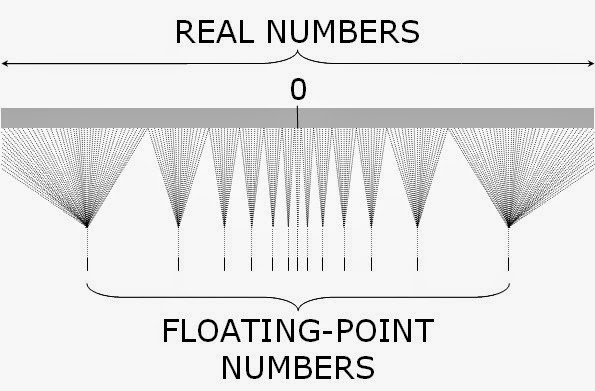
\includegraphics[width=0.5\linewidth]{Plots/U1/floatingPoint} \end{center}

\begin{itemize}
\tightlist
\item
  El \textbf{IEEE-754} define dos tipos de formatos: el de precisión simple (en el cual cada número ocupa 32 bit de memoria) y el de precisión doble (un número ocupa 64 bit).
\item
  El formato de doble precisión en 64 bit, empleado actualmente en casi todas las computadoras, tiene la siguiente estructura.
\end{itemize}

\begin{center}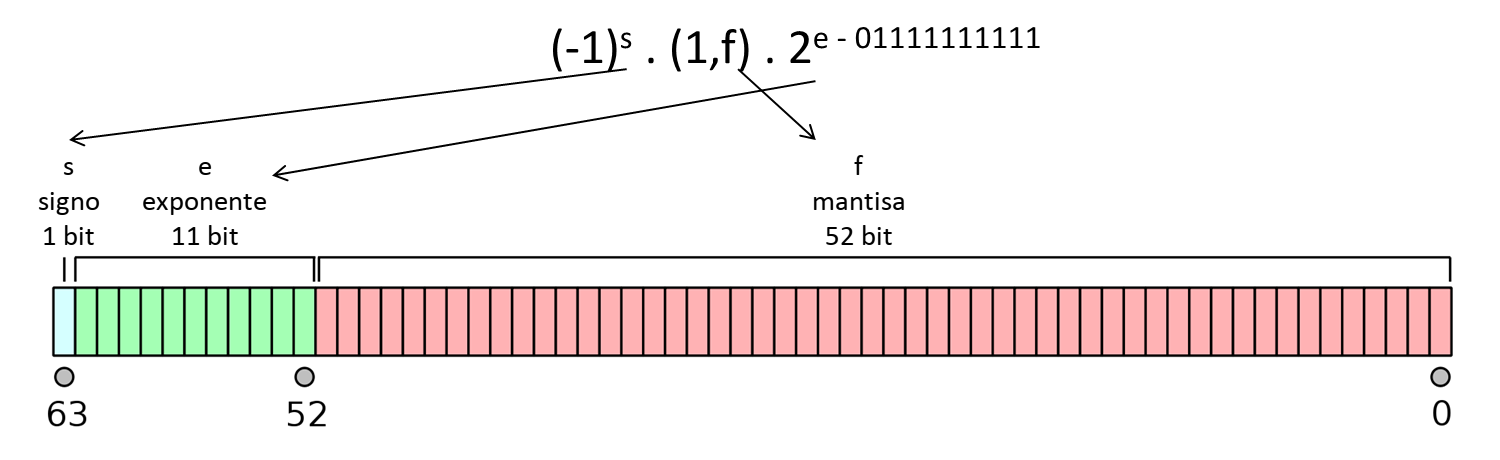
\includegraphics[width=0.9\linewidth]{Plots/U1/float64_2} \end{center}

\begin{itemize}
\item
  El bit que indica el signo, \(s\), vale 0 si el número es positivo o 1 si es negativo.
\item
  El exponente \(e\) ocupa 11 bit dando lugar a \(2^{11} = 2048\) valores distintos. Se dice que es un exponente sesgado porque se le resta \(01111111111_{(2)} = 1023_{(10)}\), por lo que puede variar entre -1023 y 1024.
\item
  La mantisa \((1,f)\) se registra \emph{normalizada}, es decir con un solo dígito antes de la coma igual a 1, de manera que dicho 1 no se almacena, es implícito. Luego de la coma, la parte fraccionaria \(f\) ocupa 52 bit (\(2^{52}\) valores distintos).
\item
  Por ejemplo, el siguiente conjunto de 64 bit representa al número decimal -74,5 (verificación opcional).
\end{itemize}

\begin{center}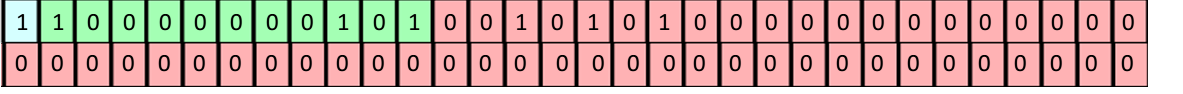
\includegraphics[width=1\linewidth]{Plots/U1/floatej} \end{center}

\begin{itemize}
\tightlist
\item
  En \href{http://weitz.de/ieee/}{este link} se puede encontrar una calculadora que convierte números entre sus representaciones en decimal y en coma flotante.
\end{itemize}

\hypertarget{propiedades-importantes-del-formato-ieee-754}{%
\section{Propiedades importantes del formato IEEE-754}\label{propiedades-importantes-del-formato-ieee-754}}

\begin{itemize}
\item
  Además de representar números, este sistema permite almacenar ciertos valores especiales. Uno de ellos es \emph{NaN} (\emph{Not a Number}), para resultados no definidos matemáticamente. Por ejemplo:

\begin{Shaded}
\begin{Highlighting}[]
\DecValTok{0}\OperatorTok{/}\DecValTok{0}
\end{Highlighting}
\end{Shaded}

\begin{verbatim}
[1] NaN
\end{verbatim}

\begin{Shaded}
\begin{Highlighting}[]
\KeywordTok{sqrt}\NormalTok{(}\OperatorTok{-}\DecValTok{1}\NormalTok{)}
\end{Highlighting}
\end{Shaded}

\begin{verbatim}
[1] NaN
\end{verbatim}

  Operaciones como \(x + NaN, NaN \times x, NaN / x, x / NaN\) resultan en \(NaN\) (excepto \(NaN^0 = 1\)).

  \textbf{Observación}: en R \texttt{NaN} no es lo mismo que \texttt{NA} (\emph{Not Available}). \texttt{NA} es una construcción de R, que no forma parte del IEEE-754, para representar valores desconocidos o faltantes.
\item
  El infinito tiene su propia representación en este estándar y puede ser positivo o negativo. Un valor infinito puede darse como resultado de ciertas operaciones o por exceder los límites de almacenamiento. En R se representan con \texttt{Inf} y \texttt{-Inf}.
\end{itemize}

\begin{Shaded}
\begin{Highlighting}[]
\OtherTok{Inf}
\end{Highlighting}
\end{Shaded}

\begin{verbatim}
[1] Inf
\end{verbatim}

\begin{Shaded}
\begin{Highlighting}[]
\OtherTok{Inf} \OperatorTok{-}\StringTok{ }\OtherTok{Inf}
\end{Highlighting}
\end{Shaded}

\begin{verbatim}
[1] NaN
\end{verbatim}

\begin{Shaded}
\begin{Highlighting}[]
\OtherTok{Inf} \OperatorTok{/}\StringTok{ }\OtherTok{Inf}
\end{Highlighting}
\end{Shaded}

\begin{verbatim}
[1] NaN
\end{verbatim}

\begin{itemize}
\tightlist
\item
  La división por cero resulta en infinito, aunque matemáticamente sea una indefinición. Y como contrapartida, dividir por infinito da cero.
\end{itemize}

\begin{Shaded}
\begin{Highlighting}[]
\DecValTok{3}\OperatorTok{/}\DecValTok{0}
\end{Highlighting}
\end{Shaded}

\begin{verbatim}
[1] Inf
\end{verbatim}

\begin{Shaded}
\begin{Highlighting}[]
\DecValTok{-3}\OperatorTok{/}\DecValTok{0}
\end{Highlighting}
\end{Shaded}

\begin{verbatim}
[1] -Inf
\end{verbatim}

\begin{Shaded}
\begin{Highlighting}[]
\DecValTok{3}\OperatorTok{/}\OtherTok{Inf}
\end{Highlighting}
\end{Shaded}

\begin{verbatim}
[1] 0
\end{verbatim}

\begin{itemize}
\tightlist
\item
  Infinito es el próximo valor al mayor valor que puede registrarse bajo este formato. En R, existe un objeto llamado \texttt{.Machine} que es una lista con información numérica de la máquina en la que se está trabajando, por ejemplo, cuál es el mayor número en coma flotante normalizada. Si a este valor lo multiplicamos, por ejemplo, por 2, tenemos infinito:
\end{itemize}

\begin{Shaded}
\begin{Highlighting}[]
\NormalTok{.Machine}\OperatorTok{$}\NormalTok{double.xmax}
\end{Highlighting}
\end{Shaded}

\begin{verbatim}
[1] 1.797693e+308
\end{verbatim}

\begin{Shaded}
\begin{Highlighting}[]
\NormalTok{.Machine}\OperatorTok{$}\NormalTok{double.xmax }\OperatorTok{*}\StringTok{ }\DecValTok{2}
\end{Highlighting}
\end{Shaded}

\begin{verbatim}
[1] Inf
\end{verbatim}

\begin{itemize}
\tightlist
\item
  El 0 tiene signo, puede ser \(+0\) o \(-0\). \(-0\) actúa como \(0\) y se muestra como \(0\), pero el signo negativo se propaga en las operaciones.
\end{itemize}

\begin{Shaded}
\begin{Highlighting}[]
\DecValTok{-0}
\end{Highlighting}
\end{Shaded}

\begin{verbatim}
[1] 0
\end{verbatim}

\begin{Shaded}
\begin{Highlighting}[]
\DecValTok{3} \OperatorTok{*}\StringTok{ }\DecValTok{-0}
\end{Highlighting}
\end{Shaded}

\begin{verbatim}
[1] 0
\end{verbatim}

\begin{Shaded}
\begin{Highlighting}[]
\DecValTok{1} \OperatorTok{/}\StringTok{ }\DecValTok{0}
\end{Highlighting}
\end{Shaded}

\begin{verbatim}
[1] Inf
\end{verbatim}

\begin{Shaded}
\begin{Highlighting}[]
\DecValTok{1} \OperatorTok{/}\StringTok{ }\DecValTok{-0}
\end{Highlighting}
\end{Shaded}

\begin{verbatim}
[1] -Inf
\end{verbatim}

\begin{itemize}
\tightlist
\item
  Como ya dijimos, bajo este sistema no podemos representar todos los números reales. El \textbf{error de máquina} o \textbf{epsilon de máquina} es una medida del espacio que hay entre dos números consecutivos en la computadora. Se define como el menor número \(\epsilon > 0\) tal que \(1 + \epsilon > 1\).
\end{itemize}

Si bien \(1 + x > 1\) debería verificarse para cualquier \(x > 0\), en la computadora no es así, porque si \(x\) es muy pequeño, \(1 + x\) será redondeado a \(1\). Por eso, el \(\epsilon\) de máquina es aquella cantidad mínima necesaria para que \(1 + \epsilon\) se distinga de \(1\).

En R, podemos averiguar el epsilon de máquina así:

\begin{Shaded}
\begin{Highlighting}[]
\NormalTok{.Machine}\OperatorTok{$}\NormalTok{double.eps}
\end{Highlighting}
\end{Shaded}

\begin{verbatim}
[1] 2.220446e-16
\end{verbatim}

Podemos usar la función \texttt{print} para elegir la cantidad de decimales que queremos ver y así experimentar con el \(\epsilon\) de máquina:

\begin{Shaded}
\begin{Highlighting}[]
\KeywordTok{print}\NormalTok{(}\DecValTok{1} \OperatorTok{+}\StringTok{ }\NormalTok{.Machine}\OperatorTok{$}\NormalTok{double.eps, }\DataTypeTok{digits =} \DecValTok{20}\NormalTok{)}
\end{Highlighting}
\end{Shaded}

\begin{verbatim}
[1] 1.000000000000000222
\end{verbatim}

\begin{Shaded}
\begin{Highlighting}[]
\KeywordTok{print}\NormalTok{(}\DecValTok{1} \OperatorTok{+}\StringTok{ }\NormalTok{.Machine}\OperatorTok{$}\NormalTok{double.eps }\OperatorTok{*}\StringTok{ }\DecValTok{2}\NormalTok{, }\DataTypeTok{digits =} \DecValTok{20}\NormalTok{)}
\end{Highlighting}
\end{Shaded}

\begin{verbatim}
[1] 1.0000000000000004441
\end{verbatim}

\begin{Shaded}
\begin{Highlighting}[]
\KeywordTok{print}\NormalTok{(}\DecValTok{1} \OperatorTok{+}\StringTok{ }\NormalTok{.Machine}\OperatorTok{$}\NormalTok{double.eps }\OperatorTok{/}\StringTok{ }\DecValTok{2}\NormalTok{, }\DataTypeTok{digits =} \DecValTok{20}\NormalTok{)}
\end{Highlighting}
\end{Shaded}

\begin{verbatim}
[1] 1
\end{verbatim}

Aunque nos parezca despreciable, esto puede ser una limitación a considerar, por ejemplo, si trabajamos con medidas de partículas subatómicas.

Si hacemos 1000 + \(\epsilon\), encontraremos que el resultado es 1000. Es decir, 1000 + \(\epsilon\) no se distingue de 1000. Es porque \(\epsilon\) está definido con respecto a 1. Como los números en coma flotante son cada vez más espaciados cuanto más nos alejamos de 0, a 1000 habrá que sumarle un \(x\) algo más grande para que \(1000 + x\) se distinga de 1000.

\begin{Shaded}
\begin{Highlighting}[]
\KeywordTok{print}\NormalTok{(}\DecValTok{1000} \OperatorTok{+}\StringTok{ }\NormalTok{.Machine}\OperatorTok{$}\NormalTok{double.eps, }\DataTypeTok{digits =} \DecValTok{20}\NormalTok{)}
\end{Highlighting}
\end{Shaded}

\begin{verbatim}
[1] 1000
\end{verbatim}

\begin{Shaded}
\begin{Highlighting}[]
\KeywordTok{print}\NormalTok{(}\DecValTok{1000} \OperatorTok{+}\StringTok{ }\DecValTok{100} \OperatorTok{*}\StringTok{ }\NormalTok{.Machine}\OperatorTok{$}\NormalTok{double.eps, }\DataTypeTok{digits =} \DecValTok{20}\NormalTok{)}
\end{Highlighting}
\end{Shaded}

\begin{verbatim}
[1] 1000
\end{verbatim}

\begin{Shaded}
\begin{Highlighting}[]
\KeywordTok{print}\NormalTok{(}\DecValTok{1000} \OperatorTok{+}\StringTok{ }\DecValTok{300} \OperatorTok{*}\StringTok{ }\NormalTok{.Machine}\OperatorTok{$}\NormalTok{double.eps, }\DataTypeTok{digits =} \DecValTok{20}\NormalTok{)}
\end{Highlighting}
\end{Shaded}

\begin{verbatim}
[1] 1000.0000000000001137
\end{verbatim}

\begin{itemize}
\tightlist
\item
  \textbf{Overflow (desbordamiento)}. Es el fenómeno que ocurre cuando un cálculo produce un resultado cuya magnitud es mayor que la que se puede almacenar o representar (en R, \texttt{.Machine\$double.xmax}). Aunque este número probablemente es mucho mayor que cualquier número que utilicemos en la práctica, debería ser tenido en cuenta, por ejemplo, si hacemos cálculos en cosmología.
\end{itemize}

\begin{Shaded}
\begin{Highlighting}[]
\NormalTok{.Machine}\OperatorTok{$}\NormalTok{double.xmax}
\end{Highlighting}
\end{Shaded}

\begin{verbatim}
[1] 1.797693e+308
\end{verbatim}

\begin{Shaded}
\begin{Highlighting}[]
\NormalTok{.Machine}\OperatorTok{$}\NormalTok{double.xmax }\OperatorTok{*}\StringTok{ }\DecValTok{2}
\end{Highlighting}
\end{Shaded}

\begin{verbatim}
[1] Inf
\end{verbatim}

\begin{itemize}
\item
  \textbf{Underflow (desbordamiento)}. Es el fenómeno que ocurre cuando cuando el resultado de una operación en coma flotante es menor en magnitud (más cercano a cero) que el menor número representable (en R, \texttt{.Machine\$double.xmin}). Es difícil mostrar un ejemplo de esto porque, dependiendo de la máquina, la representación en coma flotante puede recurrir a números no normalizados para lograr números incluso por fuera de los límites de desbordamiento:

\begin{Shaded}
\begin{Highlighting}[]
\CommentTok{# Mínimo representable en coma flotante normalizada}
\NormalTok{.Machine}\OperatorTok{$}\NormalTok{double.xmin}
\end{Highlighting}
\end{Shaded}

\begin{verbatim}
[1] 2.225074e-308
\end{verbatim}

\begin{Shaded}
\begin{Highlighting}[]
\CommentTok{# Igual es posible conseguir números menores con representación no normalizada}
\NormalTok{.Machine}\OperatorTok{$}\NormalTok{double.xmin }\OperatorTok{/}\StringTok{ }\DecValTok{2}
\end{Highlighting}
\end{Shaded}

\begin{verbatim}
[1] 1.112537e-308
\end{verbatim}

  Observación: el mínimo representable \texttt{.Machine\$double.xmin} es menor que el \(\epsilon\) de máquina ya que los números en coma flotante son más densos alrededor del 0 que del 1.
\end{itemize}

\hypertarget{anuxe1lisis-de-los-errores}{%
\section{Análisis de los errores}\label{anuxe1lisis-de-los-errores}}

\begin{itemize}
\tightlist
\item
  Como ya hemos dicho, los métodos numéricos proporcionan una solución aproximada de los problemas que tratan de resolver.
\item
  Y aunque es cierto que algunos de los métodos que se estudiarán idealmente proporcionarían una solución exacta, esto tampoco ocurrirá por las aproximaciones que realiza la computadora en la representación numérica.
\item
  Denominamos \textbf{error} a la diferencia entre la solución que los métodos, una vez programados, devuelven y la solución exacta del problema que se trata de resolver. Hay dos tipos fundamentales de errores.
\end{itemize}

\hypertarget{error-de-truncamiento}{%
\subsection{Error de truncamiento}\label{error-de-truncamiento}}

\begin{itemize}
\tightlist
\item
  Dado que un método numérico propone un algoritmo para resolver de forma aproximada un problema que no se puede resolver mediante métodos analíticos, se llama \textbf{error de truncamiento} a la diferencia entre el valor aproximado propuesto por el método y la solución exacta del problema.
\item
  Ocurre cuando un proceso que requiere un número infinito de pasos se detiene en un número finito de pasos.
\item
  Por ejemplo, podemos recordar el desarrollo en serie de Taylor de la función \(f(x) = e^{x^2}\):
\end{itemize}

\[ e^{x^2} = 1 + x^2 + \frac{x^4}{2!} + \frac{x^6}{3!} + ... + \frac{x^{2n}}{n!} + ...\]

\begin{itemize}
\tightlist
\item
  Si nos quedamos sólo con los primeros 4 términos, estamos aproximando una suma que tiene infinita cantidad de sumandos sólo con los primeros 4, de manera que dicha aproximación presentará un error de truncamiento.
\item
  Este tipo de error no depende directamente del sistema numérico que se emplee.
\end{itemize}

\hypertarget{error-de-redondeo}{%
\subsection{Error de redondeo}\label{error-de-redondeo}}

\begin{itemize}
\tightlist
\item
  Resulta de reemplazar un número por su forma en coma flotante, es decir, por su representación en la computadora mediante un número finito de bits.
\item
  Recibe este nombre ya sea que la aproximación se realice con redondeo o poda (también conocida como \emph{truncamiento}, pero no debe confundirse con el error de truncamiento).
\item
  El error de redondeo está ligado fundamentalmente al tipo de precisión que se emplee (algo determinado por el procesador y el software usados).
\item
  Sin embargo, el efecto final de los errores de redondeo depende también del algoritmo propuesto por el método numérico y por la forma de programarlo.
\item
  Existen operaciones que son especialmente sensibles a los errores de redondeo o un algoritmo puede hacer que los mismos se amplifiquen.
\end{itemize}

\hypertarget{ejemplos-de-operaciones-delicadas}{%
\subsection{Ejemplos de operaciones ``delicadas''}\label{ejemplos-de-operaciones-delicadas}}

\textbf{Sustracción de números casi iguales en valor absoluto}

\begin{itemize}
\tightlist
\item
  Da lugar a importantes pérdidas de precisión.
\item
  El resultado tiene menos cifras significativas que los valores originales (\textbf{pérdida de cifras significativas} o \textbf{cancelación catastrófica}).
\item
  Por ejemplo: sean \(p = 3.1415926536\) y \(q = 3.1415957341\).
\item
  Tienen 11 cifras significativas cada uno.
\item
  Sin embargo, \(p - q = -0.0000030805\) tiene sólo 5 cifras significativas.
\item
  Esto puede producir una reducción en la precisión final de la respuesta calculada.
\end{itemize}

\textbf{División por cantidades pequeñas}

\begin{itemize}
\tightlist
\item
  Un error mínimo en el dividendo se traduce en uno mucho mayor en el resultado, de modo que la falta de precisión podría ocasionar un \emph{overflow} o pérdida de cifras significativos.
\item
  Veremos un ejemplo de esto cuando resolvamos sistemas de ecuaciones lineales con la estrategia de pivoteo en el algoritmo de eliminación de Gauss.
\item
  Dado que los números de punto flotante están más concentrados cerca del cero entonces al dividir por un número más grande es más probable conseguir una mejor aproximación.
\end{itemize}

\textbf{Adición de un número grande y uno pequeño}

\begin{itemize}
\tightlist
\item
  Puede hacer que el pequeño desaparezca.
\item
  En ciertos casos esto no ocasiona un problema ya que, si tenemos un número de gran magnitud probablemente podamos considerar al más pequeño despreciable.
\item
  Sin embargo debe tenerse mucho cuidado con el orden de las operaciones ya que si, por ejemplo, sumamos una gran cantidad de numeros pequeños entre ellos (que juntos tienen un peso considerable) y luego se lo sumamos a un número grande, todo funcionará correctamente.
\item
  Pero si vamos sumando uno por uno los números pequeños al grande entonces en cada paso el número pequeño será considerado despreciable y llegaremos a un resultado erróneo.
\end{itemize}

\hypertarget{medida-del-error}{%
\subsection{Medida del error}\label{medida-del-error}}

Existen dos formas fundamentales de medir los errores que se cometen en la aproximación de la solución de un problema mediante un método numérico. Siendo \(x\) el valor exacto y \(\hat{x}\) su aproximación, definimos:

\begin{itemize}
\item
  \textbf{Error absoluto}: \(E_a = |x - \hat{x}|\). Se mide en las mismas unidades de la variable que se trata de aproximar (por ejemplo, en amperios si se quiere aproximar la corriente que circula por un circuito eléctrico).
\item
  \textbf{Error relativo}: \(E_r = \frac{|x - \hat{x}|}{|x|}, x\neq 0\). Relaciona el error obtenido con la magnitud de la propia solución y se interpreta como porcentaje. Esta medida del error es invariante a los cambios de escala, ya que es independiente de las unidades de medida.
\end{itemize}

\hypertarget{error-propagado}{%
\subsection{Error propagado}\label{error-propagado}}

\begin{itemize}
\tightlist
\item
  Se define como \textbf{error propagado} al error que se tiene al final de una cadena de operaciones sucesivas por la existencia de diferentes errores en los pasos intermedios.
\item
  Por ejemplo, si tenemos dos valores exactos \(p\) y \(q\) con valores aproximados \(\hat{p}\) y \(\hat{q}\) cuyos errores son \(\epsilon_p\) y \(\epsilon_q\) de modo que \(\hat{p} = p + \epsilon_p\) y \(\hat{q} = q + \epsilon_q\), al realizar la suma entre los valores aproximados:
\end{itemize}

\[\hat{p} + \hat{q} = (p + \epsilon_p) + (q + \epsilon_q) = (p + q) + (\epsilon_p + \epsilon_q)\]

\begin{itemize}
\item
  Si bien es normal que en una cadena los errores iniciales se propaguen, es deseable que un error pequeño en el comienzo produzca errores pequeños en el resultado final.
\item
  Un algoritmo con esta cualidad se llama \textbf{estable} (el error se puede acotar), en caso contrario se dice \textbf{inestable}.
\item
  Supongamos que \(\epsilon\) representa un error inicial y que \(\epsilon (n)\) representa el crecimiento de dicho error después de \(n\) operaciones:

  \begin{itemize}
  \tightlist
  \item
    Si \(|\epsilon (n)| \propto n \epsilon\), el crecimiento es \textbf{lineal}.
  \item
    Si \(|\epsilon (n)| \propto k^n \epsilon\), el crecimiento es \textbf{exponencial}.

    \begin{itemize}
    \tightlist
    \item
      Si \(k > 1\), el error crece cuando \(n \rightarrow \infty\) sin que podamos acotarlo, el proceso es inestable.
    \item
      Si \(0 < k < 1\), el error decrece cuando \(n \rightarrow \infty\), se puede acotar, el proceso es estable.
    \end{itemize}
  \end{itemize}
\end{itemize}

\hypertarget{soluciuxf3n-numuxe9rica-de-ecuaciones-no-lineales}{%
\chapter{Solución Numérica de Ecuaciones No Lineales}\label{soluciuxf3n-numuxe9rica-de-ecuaciones-no-lineales}}

\hypertarget{generalidades}{%
\section{Generalidades}\label{generalidades}}

\begin{itemize}
\item
  En esta unidad estudiaremos uno de los problemas más básicos y antiguos de la aproximación numérica: la \textbf{solución de ecuaciones}.
\item
  Consiste en obtener una solución de una ecuación \(F(x) = O\).
\item
  Se presenta en una gran variedad de problemas.
\item
  Las soluciones de una ecuación se llaman \textbf{raíces} o \textbf{ceros}.
\item
  Una \textbf{ecuación lineal} es una igualdad que involucra una o más variables elevadas a la primera potencia y no contiene productos entre las variables (involucra solamente sumas y restas de las variables). Por ejemplo: \(3x+2 = 8\).
\item
  Para este tipo de ecuaciones es posible hallar analíticamente una expresión para su solución.
\item
  En una \textbf{ecuación no lineal} las incógnitas están elevadas a potencias distintas de \(1\), aparecen en denominadores o exponentes o están afectadas por funciones no lineales (como el logaritmo o las trigonométricas).
\item
  Un tipo de ecuación no lineal es la \textbf{ecuación algebraica}, que se trata de un polinomio igualado a cero:

  \[
    P_n(x) = a_0 x^n + a_1 x^{n-1} + ... + a_{n-1} x + a_n = 0
    \]
  donde \(a_0 \ne 0, n \in \mathbb{N}\) y \(a_0, \dots, a_n\) son constantes.
\item
  Ejemplo: \(x^3 - x^2 + 5x - 8 = 2x^5\).
\item
  Sabemos que si, por ejemplo, \(n = 2\), la solución de \(ax^2 + b x + c = 0\) está dada por la resolvente:
\end{itemize}

\[
x_{1,2} = \frac{b \pm \sqrt{b^2 - 4ac}}{2a}
\]

\begin{itemize}
\item
  Sin embargo, la solución análitica para este tipo de ecuaciones existe sólo para \(n \le 4\).
\item
  Las restantes ecuaciones no lineales se dice que son \textbf{trascendentes}, por ejemplo:
\end{itemize}

\begin{gather*}
x^3 - ln x + \frac{3}{x} = 2 \\
tg(x + 45) = 1 + sen(2x) \\
xe^{x}=1 \\
{\displaystyle 5^{x}=9^{x+1} 3^{x}}
\end{gather*}

\begin{itemize}
\item
  En general, tampoco es posible hallar de manera análitica una solución exacta para estas ecuaciones.
\item
  Excepto para algunos problemas, las ecuaciones no lineales carecen de solución exacta, por lo que requieren ser resueltas con métodos numéricos.
\item
  Una técnica fundamental de los métodos numéricos es la \textbf{ITERACIÓN} (métodos iterativos).
\item
  Se trata de \textbf{repetir un proceso} hasta que se obtiene un resultado para el problema.
\item
  En la unidad se verán distintos métodos iterativos para encontrar las raíces, cada con sus propias ventajas y limitaciones.
\item
  Requieren dos pasos generales:

  \begin{enumerate}
  \def\labelenumi{\arabic{enumi}.}
  \tightlist
  \item
    Determinación de un valor aproximado de la raiz que se busca.
  \item
    Mejoramiento de la solución hasta lograr un grado de precisión preestablecido.
  \end{enumerate}
\end{itemize}

\hypertarget{muxe9todo-de-las-aproximaciones-sucesivas-o-del-punto-fijo}{%
\section{Método de las Aproximaciones Sucesivas o del Punto Fijo}\label{muxe9todo-de-las-aproximaciones-sucesivas-o-del-punto-fijo}}

\hypertarget{punto-fijo}{%
\subsection{Punto fijo}\label{punto-fijo}}

\textbf{Definición de Punto Fijo}

\begin{itemize}
\item
  Un punto fijo de una función \(f(x)\) es un número real \(P\) tal que \(f(P)=P\).
\item
  Ejemplos:

  \begin{itemize}
  \tightlist
  \item
    \(f(x)=x^{2}-3x+4\), \(2\) es un punto fijo de \(f\) porque \(f(2) = 2\).
  \item
    \(f(x)=x^{2}\), \(0\) y \(1\) son puntos fijos de \(f\) porque \(f(0) = 0\) y \(f(1) = 1\).
  \end{itemize}
\end{itemize}

\textbf{¿Cómo encontrar un punto fijo de \(f(x)\)?}

Sea \(f\) una función continua y \(p_0, p_1, \dots, p_n, \dots\) una sucesión generada a partir de \(p_{n} = f(p_{n-1})\) con un valor inicial \(p_0\), es decir:

\begin{gather*}
p_0 \\
p_1 = f(p_0) \\
p_2 = f(p_1) \\
\vdots \\
p_n = f(p_{n-1}) \\
\vdots \\
\end{gather*}

Si \(lim_{n\to\infty} p_n = P\), entonces \(P\) es un punto fijo de \(f(x)\).

\hypertarget{empleo-del-punto-fijo-para-la-resoluciuxf3n-de-ecuaciones}{%
\subsection{Empleo del punto fijo para la resolución de ecuaciones}\label{empleo-del-punto-fijo-para-la-resoluciuxf3n-de-ecuaciones}}

Siendo:

\begin{equation}
F(x) = 0
\label{eq:a}
\end{equation}

la ecuación a resolver, el \textbf{Método de las Aproximaciones Sucesivas} propone reescribirla a través de la ecuación equivalente:

\[
f(x) = x
\]

de manera que la tarea de hallar un valor de \(x\) que satisface \eqref{eq:a} es lo mismo que hallar un punto fijo de la función \(f(x)\).

Entonces, el método para resolver \(F(x) = 0\) consiste en:

\begin{enumerate}
\def\labelenumi{\arabic{enumi}.}
\tightlist
\item
  Expresar la ecuación en la forma \(x = f(x)\).
\item
  Elegir un valor inicial adecuado \(x_0\).
\item
  Realizar el siguiente cálculo iterativo:
\end{enumerate}

\begin{gather*}
x_1 = f(x_0) \\
x_2 = f(x_1) \\
\vdots \\
x_n = f(x_{n-1}) \\
\vdots \\
\end{gather*}

\begin{itemize}
\tightlist
\item
  Si a medida que \(n\) crece los \(x_n\) se aproximan a un valor fijo, se dice que el método converge y la iteración se detiene cuando la diferencia entre dos valores consecutivos \(x_{n-1}\) y \(x_n\) sea tan pequeña como se desee.
\item
  El valor \(x_n\) será una raíz aproximada de \(F(x)\).
\end{itemize}

\hypertarget{ejemplo}{%
\paragraph{Ejemplo}\label{ejemplo}}
\addcontentsline{toc}{paragraph}{Ejemplo}

\begin{itemize}
\tightlist
\item
  Hallar las raíces de la ecuación no lineal: \(F(x) = x^2-3x+e^x-2=0\)
\item
  Graficamos y vemos que las raíces están cercanas a -0.4 y 1.4.
\end{itemize}

\begin{center}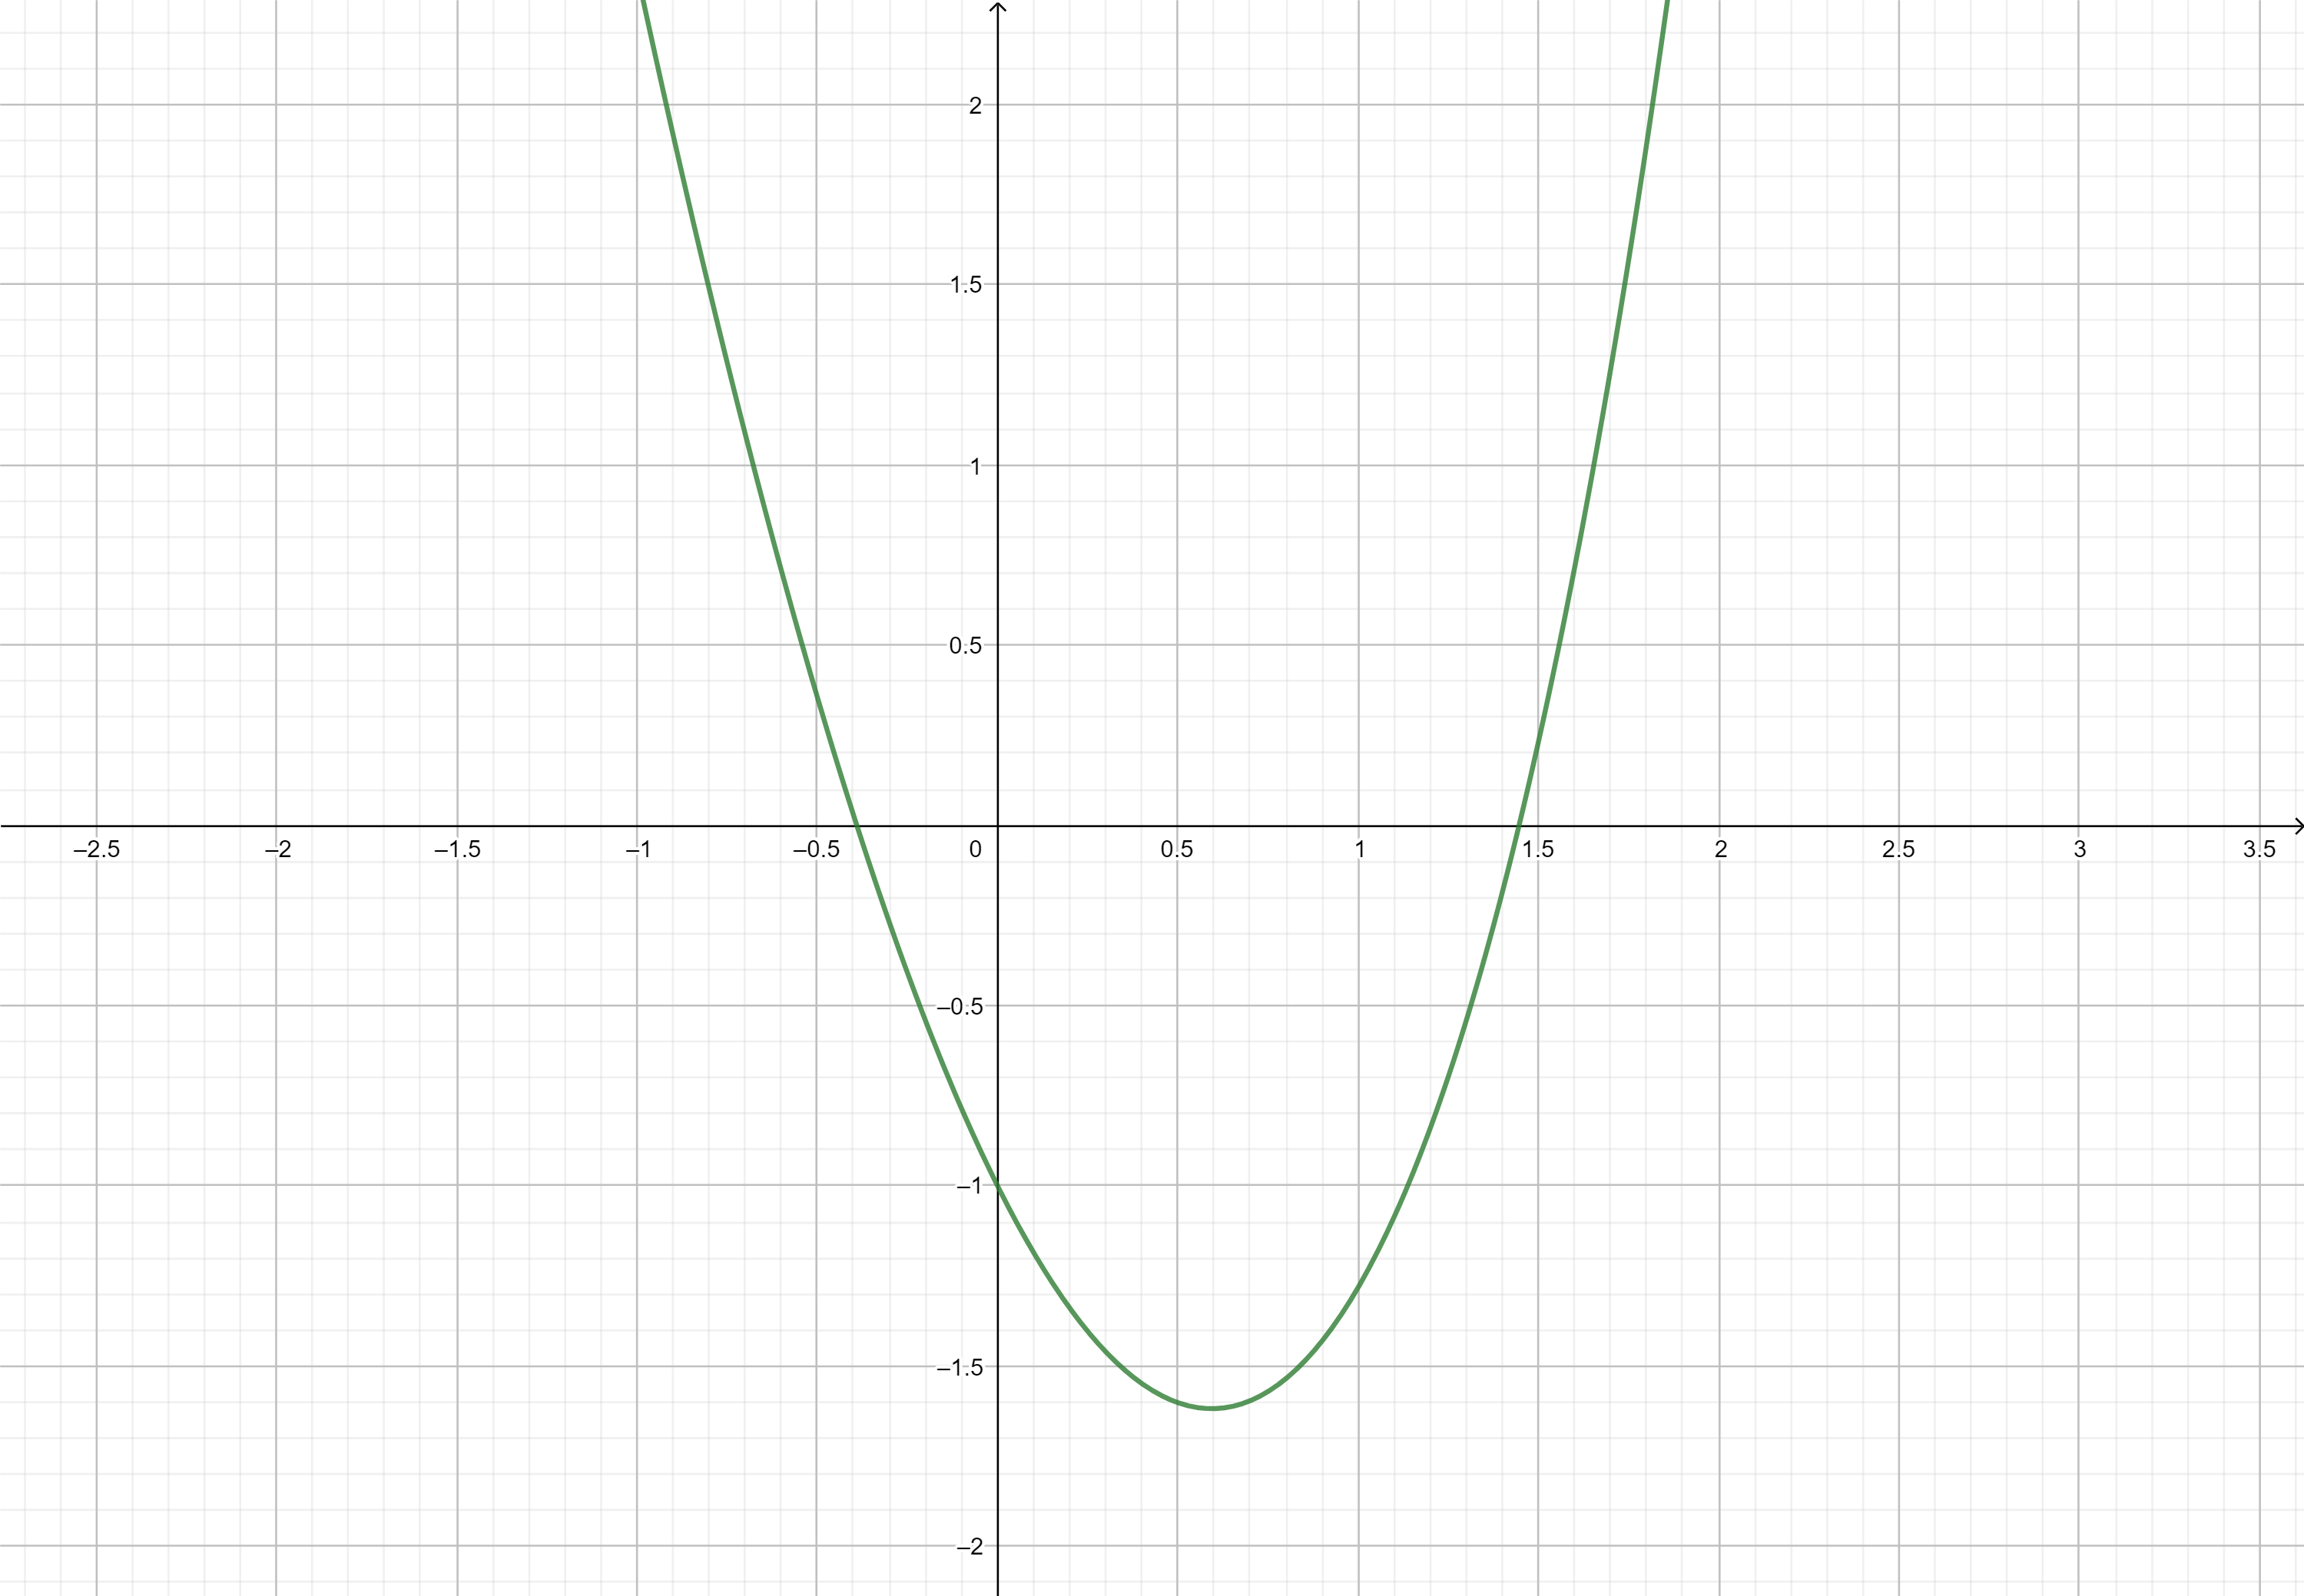
\includegraphics[width=0.7\linewidth]{Plots/U2/f1} \end{center}

\begin{itemize}
\item
  Nota: para hacer representaciones gráficas de funciones con rapidez y sencillez pueden utilizar herramientas disponibles online. Por ejemplo, nos gusta mucho usar \href{https://www.geogebra.org/graphing?lang=en}{Geogebra}.
\item
  Reescribimos \(F(x) = 0\) como \(f(x) = x\)
\item
  Por ejemplo:
\end{itemize}

\[F(x) = x^2-3x+e^x-2 = 0\]
\[\implies \underbrace{\frac{x^2+e^x-2}{3}}_{f(x)} = x \]
\[\implies f(x)= \frac{x^2+e^x-2}{3}\]

\begin{itemize}
\tightlist
\item
  Para \(x_0 = -1.5\), el proceso converge al valor -0.390271 que consideraremos como la aproximación para la raíz buscada.
\end{itemize}

\begin{center}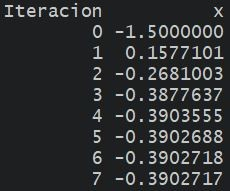
\includegraphics[width=0.4\linewidth]{Plots/U2/rtdo1} \end{center}

\begin{itemize}
\tightlist
\item
  Verificar estos resultados, pueden hacerlo rápidamente en una planilla de Excel.
\end{itemize}

\hypertarget{criterios-para-detener-el-proceso-iterativo}{%
\subsection{Criterios para detener el proceso iterativo}\label{criterios-para-detener-el-proceso-iterativo}}

\begin{itemize}
\tightlist
\item
  \textbf{Criterios para convergencia:}
\end{itemize}

\begin{enumerate}
\def\labelenumi{\arabic{enumi}.}
\item
  Error absoluto: \(|x_{j+1}-x_j| < \epsilon\)
\item
  Error relativo: \(\left|\frac{x_{j+1}-x_j}{x_j}\right| < \epsilon\)
\item
  Error relativo respecto al valor inicial: \(\left|\frac{x_{j+1}-x_j}{x_0}\right| < \epsilon\)
\item
  \(|F(x_j)| < \epsilon\)
\end{enumerate}

\begin{itemize}
\tightlist
\item
  \textbf{Criterios para divergencia}:
\end{itemize}

\begin{enumerate}
\def\labelenumi{\arabic{enumi}.}
\item
  \(j > r\), \(r\) número máximo de iteraciones
\item
  \(|x_j - x_1| > k\)
\item
  \(|F(x_j)| > k\)
\item
  \(|x_{j+1}-x_j| > k\)
\item
  \(\left|\frac{x_{j}}{x_1}\right| > k\)
\end{enumerate}

\hypertarget{ejemplo-1}{%
\subsubsection*{Ejemplo}\label{ejemplo-1}}
\addcontentsline{toc}{subsubsection}{Ejemplo}

\begin{itemize}
\tightlist
\item
  En cada paso calculamos el error relativo y nos detuvimos cuando el mismo fue menor a 1E-6.
\end{itemize}

\begin{center}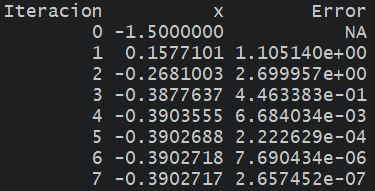
\includegraphics[width=0.5\linewidth]{Plots/U2/rtdo} \end{center}

\hypertarget{teorema-del-punto-fijo}{%
\subsection{Teorema del Punto Fijo}\label{teorema-del-punto-fijo}}

\begin{itemize}
\tightlist
\item
  Pero esto no funciona siempre, para cualquier \(f\) o cualquier \(x_0\)\ldots{}
\item
  ¿Cuándo funciona? Cuando se cumplen las condiciones del \textbf{Teorema del Punto Fijo}.
\item
  A saber:
\end{itemize}

Dadas las siguientes condiciones:

\begin{enumerate}
\def\labelenumi{\alph{enumi}.}
\tightlist
\item
  \(f\) es una función continua en el intervalo \([a, b]\)
\item
  \(f(x) \in [a, b] \quad \forall x \in [a, b]\)
\item
  \(f'\) existe en \((a, b)\) con \(|f'(x)| \le m < 1 \quad \forall x \in (a, b)\)
\end{enumerate}

Si \(x_0\) es cualquier número en \([a, b]\), entonces la sucesión definida por
\[ x_n = f(x_{n-1}), \quad n \ge 1,\]

converge al único punto fijo que \(f\) posee en \([a, b]\).

Ver demostración en el anexo.

\hypertarget{ejemplo-4}{%
\subsubsection*{Ejemplo}\label{ejemplo-4}}
\addcontentsline{toc}{subsubsection}{Ejemplo}

\begin{itemize}
\tightlist
\item
  En el ejemplo anterior, dada la ecuación \(F(x) = x^2-3x+e^x-2=0\), la reexpresamos como:
\end{itemize}

\[x = \frac{x^2+e^x-2}{3} \implies f(x)= \frac{x^2+e^x-2}{3}\]

\[\implies f'(x) = \frac{1}{3}(2x+e^x)\]

\begin{itemize}
\tightlist
\item
  Verificar condiciones del Teorema: para cada región donde se encuentra la raíz, tomar un intervalo \([a, b]\) que la cubra y graficar \(f\) y su derivada para poder observar el cumplimiento o no de las condiciones.
\item
  Si no se cumplen las condiciones, podemos probar con otra expresión para \(f(x)\).
\end{itemize}

\hypertarget{interpretaciuxf3n-gruxe1fica}{%
\subsection{Interpretación gráfica}\label{interpretaciuxf3n-gruxe1fica}}

\begin{itemize}
\tightlist
\item
  Dado que el método plantea encontrar el valor de \(x\) que satisface \(x = f(x)\), resolver la ecuación original es equivalente a resolver el sistema:
\end{itemize}

\begin{equation}
  \begin{cases}
    y = f(x) \\
    y = x
  \end{cases}
\end{equation}

\begin{itemize}
\tightlist
\item
  Es decir, que geométricamente el valor buscado es el punto de intersección de la curva \(y=f(x)\) con la recta \(y=x\).
\end{itemize}

\hypertarget{ejemplo-5}{%
\subsubsection*{Ejemplo}\label{ejemplo-5}}
\addcontentsline{toc}{subsubsection}{Ejemplo}

\begin{itemize}
\tightlist
\item
  Para \(x_0 = -1.5\), el proceso converge en 7 iteraciones a la raíz -0.390271 con un error relativo menor a -1E+6.
\end{itemize}

\begin{center}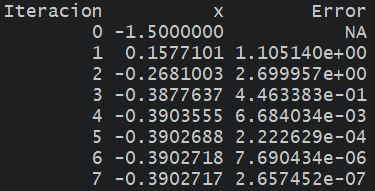
\includegraphics[width=0.6\linewidth]{Plots/U2/rtdo} \end{center}

\begin{center}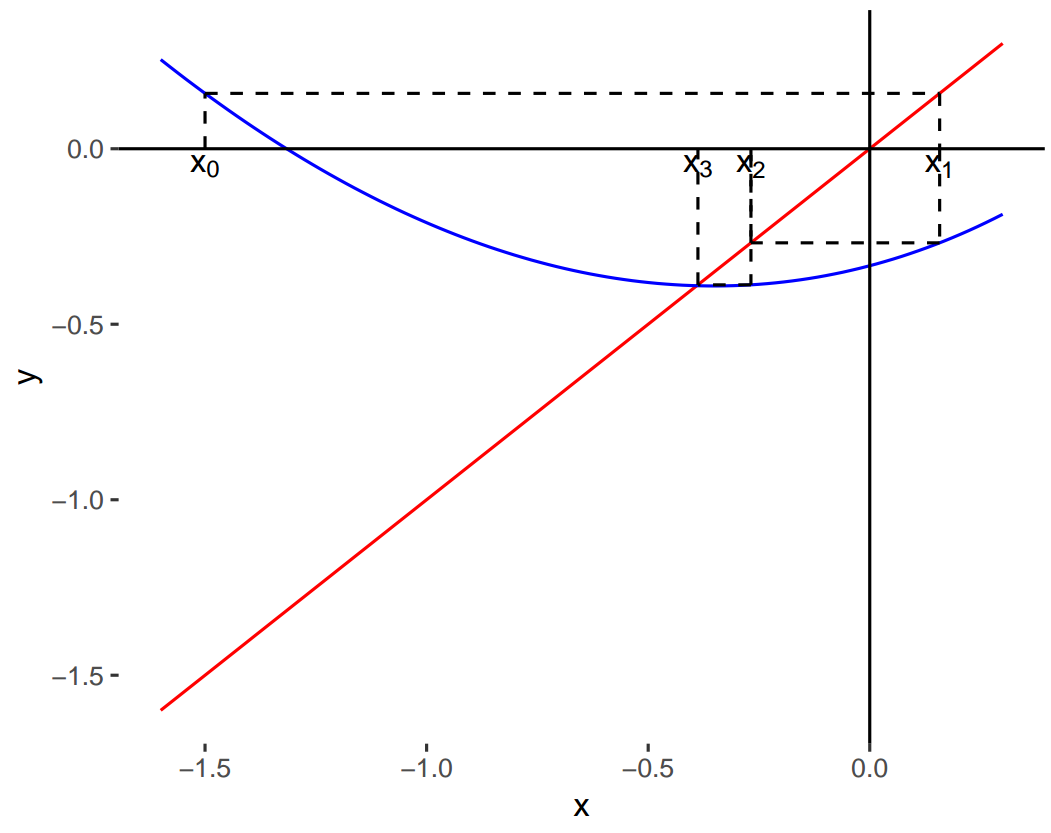
\includegraphics[width=1\linewidth]{Plots/U2/f3} \end{center}

\hypertarget{algunos-diagramas}{%
\subsection{Algunos diagramas}\label{algunos-diagramas}}

\textbf{Ejemplos de convergencia:}

\begin{center}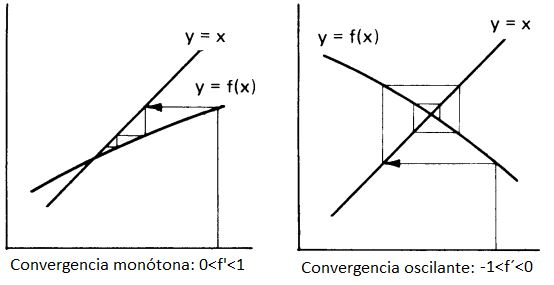
\includegraphics[width=0.75\linewidth]{Plots/U2/convergencia} \end{center}

\textbf{Ejemplos de divergencia:}

\begin{center}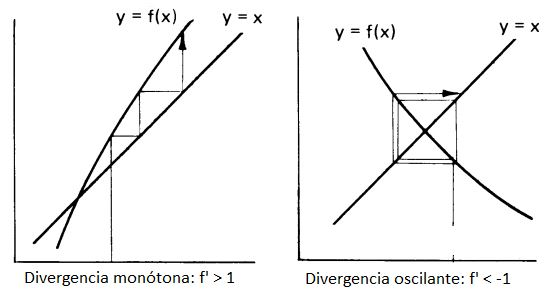
\includegraphics[width=0.75\linewidth]{Plots/U2/divergencia} \end{center}

\hypertarget{muxe9todo-de-newton-raphson}{%
\section{Método de Newton-Raphson}\label{muxe9todo-de-newton-raphson}}

\begin{itemize}
\item
  Si la función \(F\) y sus derivadas \(F'\) y \(F''\) son continuas cerca de una raíz \(p\), se pueden usar estas características de \(F\) para desarrollar algoritmos que produzcan sucesiones \(\{x_k\}\) que converjan a \(p\) más rápidamente.
\item
  El método de \textbf{Newton-Raphson} es uno de los más útiles y conocidos.
\item
  Vamos a introducir este método a partir de su interpretación geométrica y su representación gráfica.
\item
  \textbf{Recordar}: La \emph{tangente} a una curva en un punto es una recta que toca a la curva sólo en dicho punto.
\item
  Veamos el siguiente ejemplo donde el objetivo es hallar la raiz de la función \(F\), es decir, el valor \(p\) tal que \(F(p) = 0\).
\item
  (Sí, tenemos que hacer más lindos estos esquemas, ya los vamos a reemplazar por alguna animación\ldots{})
\item
  Supongamos que contamos con una aproximación inicial \(x_0\) cercana a la raiz \(p\).
\end{itemize}

\begin{center}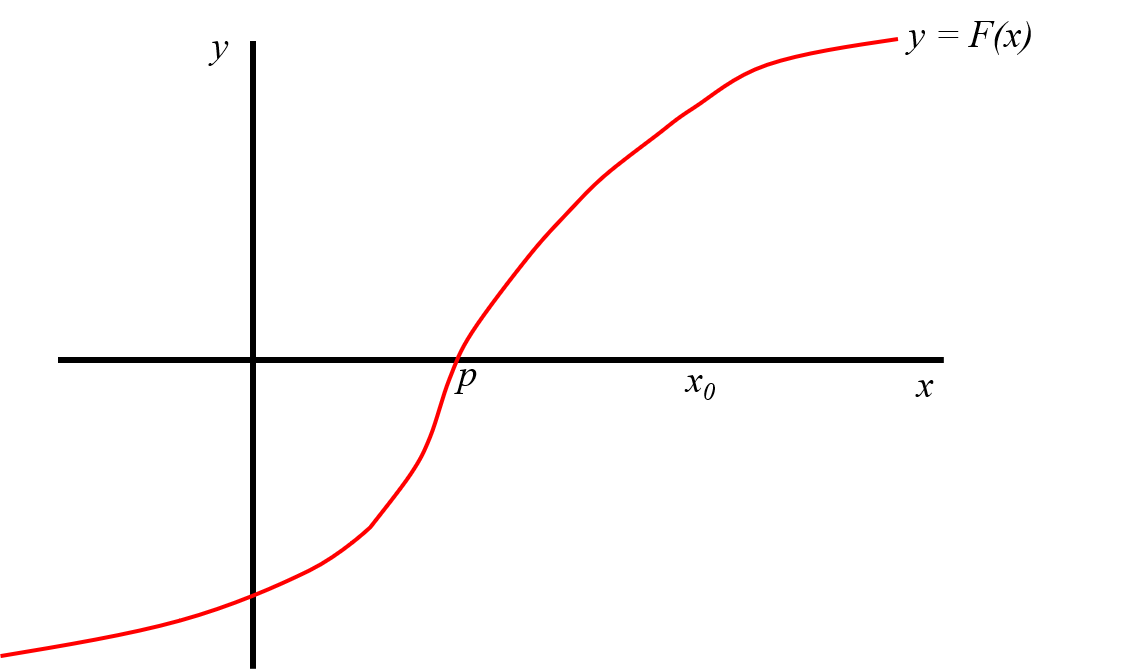
\includegraphics[width=0.9\linewidth]{Plots/U2/nr1} \end{center}

\begin{itemize}
\tightlist
\item
  Definimos a \(x_1\) como el punto de intersección del eje de las abscisas con la recta tangente a la curva \(F\) en \(x_0\).
\item
  En el caso que muestra la figura, se puede observar que \(x_1\) está más cerca de \(p\) que \(x_0\).
\end{itemize}

\begin{center}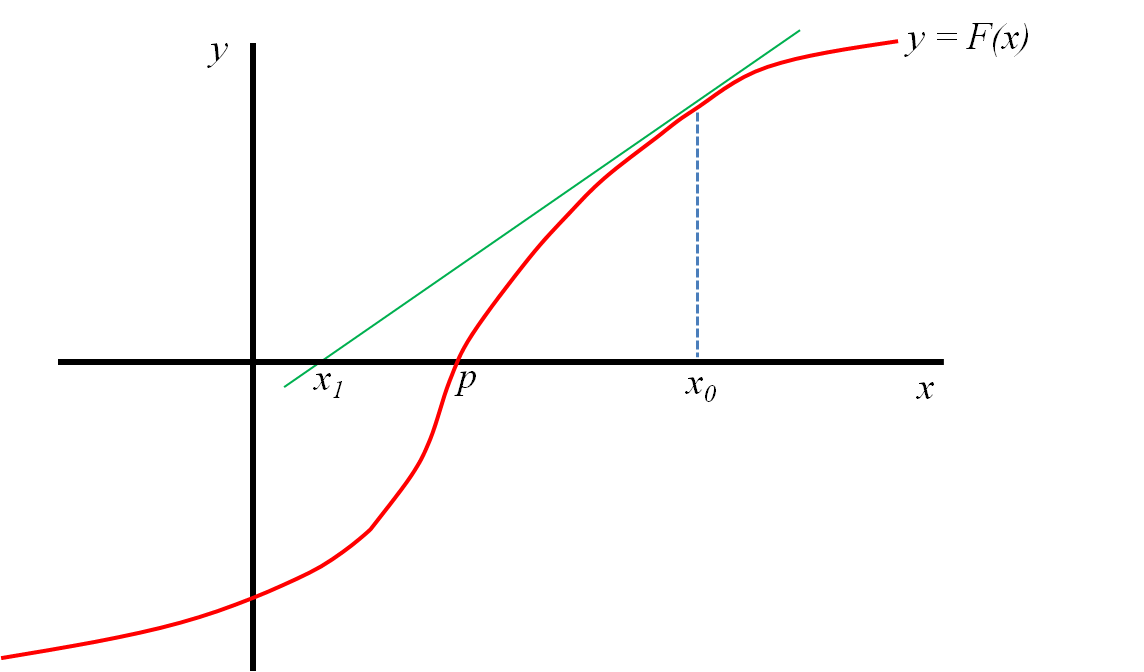
\includegraphics[width=0.9\linewidth]{Plots/U2/nr2} \end{center}

\begin{itemize}
\tightlist
\item
  Ahora definimos a \(x_2\) como el punto de intersección del eje de las abscisas con la recta tangente a la curva \(F\) en \(x_1\).
\end{itemize}

\begin{center}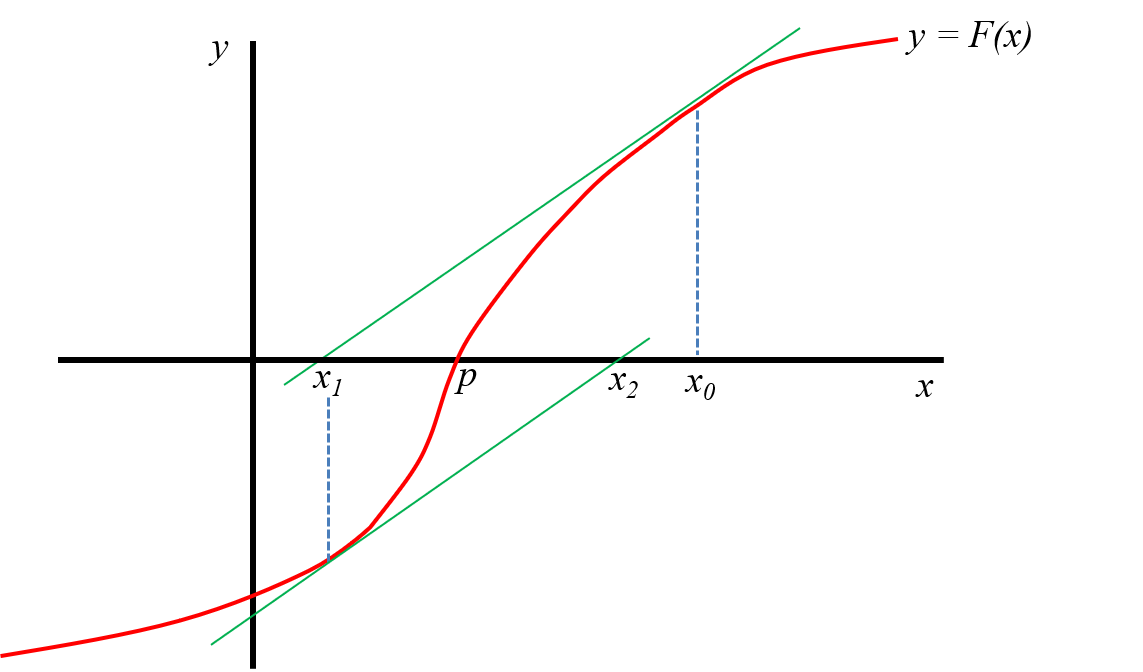
\includegraphics[width=0.9\linewidth]{Plots/U2/nr3} \end{center}

\begin{itemize}
\tightlist
\item
  Nuevamente, para el caso del ejemplo, podemos ver cómo \(x_2\) está aún más cerca de \(p\).
\item
  Si continuamos repitiendo este proceso, esperamos encontrar un \(x_n\) que sea una buena aproximación para \(p\).
\end{itemize}

\begin{center}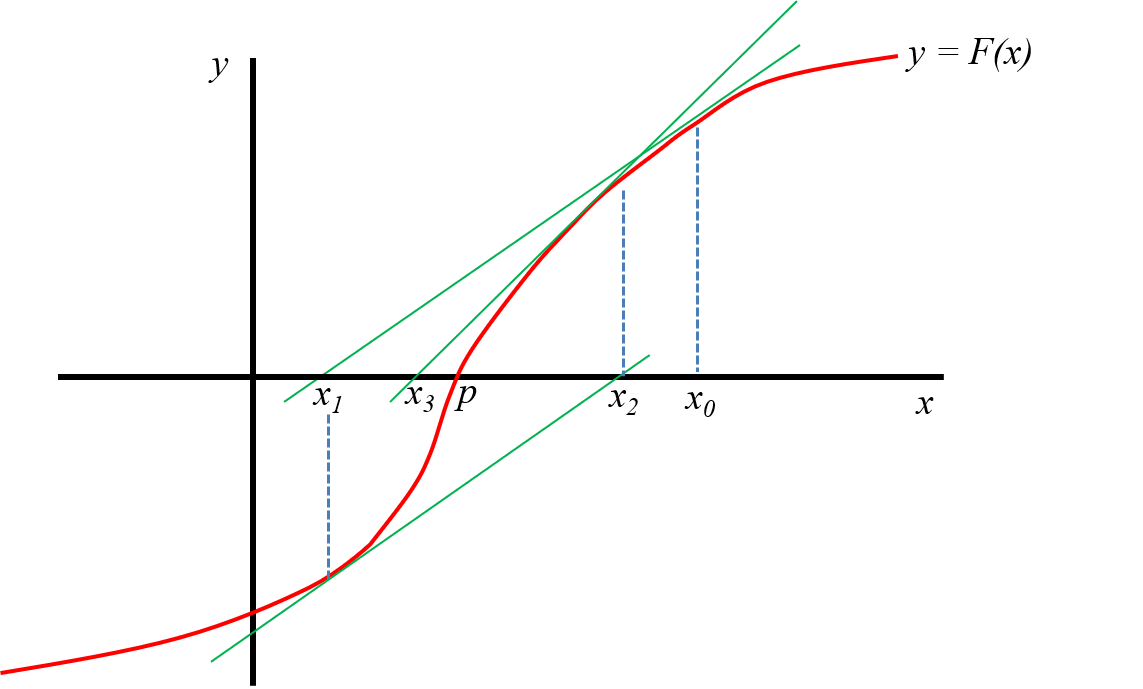
\includegraphics[width=0.9\linewidth]{Plots/U2/nr4} \end{center}

\begin{center}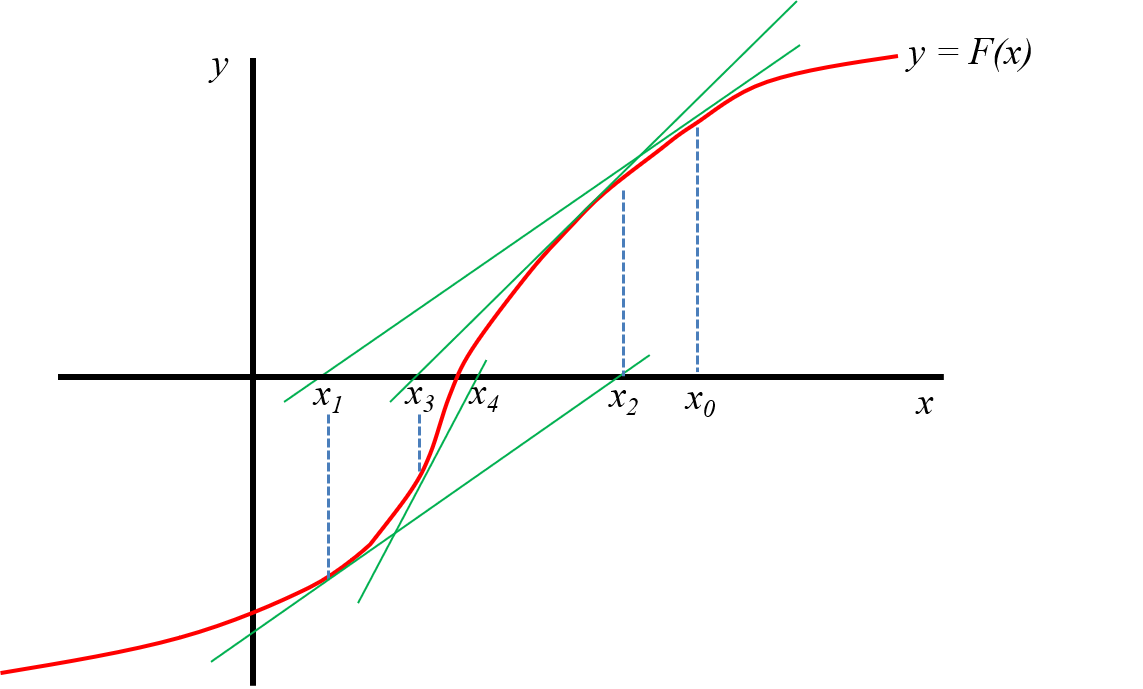
\includegraphics[width=0.9\linewidth]{Plots/U2/nr} \end{center}

\begin{itemize}
\item
  ¿Podemos expresar esto que observamos gráficamente a través de una fórmula?
\item
  Es decir, a partir de \(x_0\), ¿podemos encontrar una fórmula para \(x_1\)?
\item
  Sí, para eso hay prestarle atención a la pendiente \(m\) de la recta tangente en \(x_0\).
\item
  Por un lado, sabemos que la pendiente de la recta tangente a la curva en un punto es igual a la derivada de la función en dicho punto:

  \begin{equation}
    m = F'(x_0)
    \label{eq:deriv1}
    \end{equation}
\item
  Pero además sabemos que para cualquier recta, la pendiente es igual a:

  \begin{equation}
    m = \frac{y_1 - y_0}{x_1 - x_0}
    \label{eq:deriv2}
    \end{equation}

  siendo \((x_0, y_0)\) y \((x_1, y_1)\) dos puntos distintos que pertenecen a la misma.
\item
  Para expresar la pendiente de la recta tangente en \(x_0\), podemos tomar los puntos \((x_0, F(x_0))\) y \((x_1, 0)\) (el punto donde la tangente intersecta al eje x), de manera que a partir de la fórmula anterior:

  \begin{equation}
    m = \frac{0 - F(x_0)}{x_1 - x_0} = - \frac{F(x_0)}{x_1 - x_0}
    \label{eq:deriv3}
    \end{equation}
\item
  Igualando \eqref{eq:deriv1} y \eqref{eq:deriv3} y despejando \(x_1\) nos queda:

  \begin{equation}
    x_1 = x_0 - \frac{F(x_0)}{F'(x_0)}
    \label{eq:deriv4}
    \end{equation}
\item
  Si repetimos este pensamiento empezando desde \(x_1\) con la recta tangente a \(F\) en el punto \(x_1\), vamos a encontrar que:

  \begin{equation}
    x_2 = x_1 - \frac{F(x_1)}{F'(x_1)}
    \label{eq:deriv5}
    \end{equation}
\item
  De esta manera hemos deducido una fórmula recursiva que nos permitirá hallar una aproximación para el verdadero valor de la raiz de \(F\).
\item
  Las ideas anteriores se formalizan analíticamente a través del siguiente teorema, en el cual se deduce la fórmula recursiva a partir del desarrollo en serie de Taylor de la función \(F\).
\end{itemize}

\hypertarget{teorema-de-newton-raphson}{%
\subsection{Teorema de Newton-Raphson}\label{teorema-de-newton-raphson}}

Supongamos que la función \(F\) es continua, con derivada segunda continua en el intervalo \([a; b]\), y que existe un número \(p \in [a; b]\) tal que \(F(p) = 0\). Si \(F'(p) \neq 0\), entonces existe \(\delta > 0\) tal que la sucesión \(\{x_k\}_{k=0}^{\infty}\) definida por el proceso iterativo

\[
x_k = x_{k-1} - \frac{F(x_{k-1})}{F'(x_{k-1})} \quad k = 1, 2, \dots
\]

converge a \(p\) cualquiera sea la aproximación inicial \(x_0 \in [p - \delta; p + \delta]\)

\hypertarget{convergencia}{%
\subsubsection*{Convergencia}\label{convergencia}}
\addcontentsline{toc}{subsubsection}{Convergencia}

\textbf{Observación}: para garantizar la convergencia, \(\delta\) debe ser elegido tal que:
\[\frac{|F(x)F''(x)|}{[F'(x)]^2} < 1  \quad \forall x \in [p - \delta, p + \delta]\]

Esto significa que:

\begin{itemize}
\tightlist
\item
  \(x_0\) debe estar suficientemente cerca a la raíz de \(F(x) = 0\).
\item
  \(F''(x)\) no debe ser excesivamente grande.
\item
  \(F'(x)\) no debe estar muy próxima a cero.
\end{itemize}

\hypertarget{ejemplo-6}{%
\subsubsection*{Ejemplo}\label{ejemplo-6}}
\addcontentsline{toc}{subsubsection}{Ejemplo}

\begin{itemize}
\tightlist
\item
  Evaluar si Newton-Raphson permite hallar la raíz positiva de \(F(x) = x^2-3x+e^x-2\), que no pudo ser hallada con Aproximaciones Sucesivas.
\end{itemize}

\hypertarget{ventajas-y-desventajas}{%
\subsection{Ventajas y desventajas}\label{ventajas-y-desventajas}}

\textbf{Ventajas}

\begin{itemize}
\tightlist
\item
  Aparece la expresión original \(F\) en lugar de tener que buscar una \(f\).
\item
  Converge más rápido que el método de las aproximaciones sucesivas.
\item
  En algunos casos en que aproximaciones sucesivas diverge, N-R converge.
\item
  Se puede adaptar para hallar raíces complejas.
\end{itemize}

\textbf{Limitaciones}

\begin{itemize}
\tightlist
\item
  Si \(x_0\) está demasiado lejos de la raíz deseada, la sucesión \(\{x_k\}\) puede converger a otra raíz (la pendiente \(F'(x_0)\) es muy pequeña).
\item
  Obtener la derivada primera de la función \(F\) puede ser difícil o imposible. En ese caso se podría aproximar \(F'(x_{k-1})\) con:
  \[F'(x_{k-1}) \approx \frac{F(x_{k-1} + h) - F(x_{k-1})}{h}\]
  donde \(h\) es un valor pequeño, por ejemplo, \(h = 0,001\).
\end{itemize}

\hypertarget{muxe9todo-de-von-mises}{%
\section{Método de von Mises}\label{muxe9todo-de-von-mises}}

\begin{itemize}
\tightlist
\item
  En el método de N-R, el denominador \(F'(x_k)\) hace que geométricamente se pase de una aproximación a la siguiente por la tangente de la curva \(y = F(x)\) en el punto correspondiente a la aproximación presente \(x_k\).
\item
  Esto puede producir problemas cuando se esté en puntos alejados de raíces y cerca de puntos donde el valor de \(F'(x)\) sea cercano a 0 (tangentes cercanas a la horizontal).
\item
  Para resolver este problema, von Mises sugirió sustituir \(F'(x_k)\) en el denominador por \(F'(x_0)\).
\item
  Es decir, obtener geométricamente las siguientes aproximaciones por medio de rectas paralelas siempre a la primera tangente.
\item
  La fórmula de recurrencia resultante es:
\end{itemize}

\[
x_k = x_{k-1} - \frac{F(x_{k-1})}{F'(x_{0})} \quad k = 1, 2, \dots
\]

\begin{center}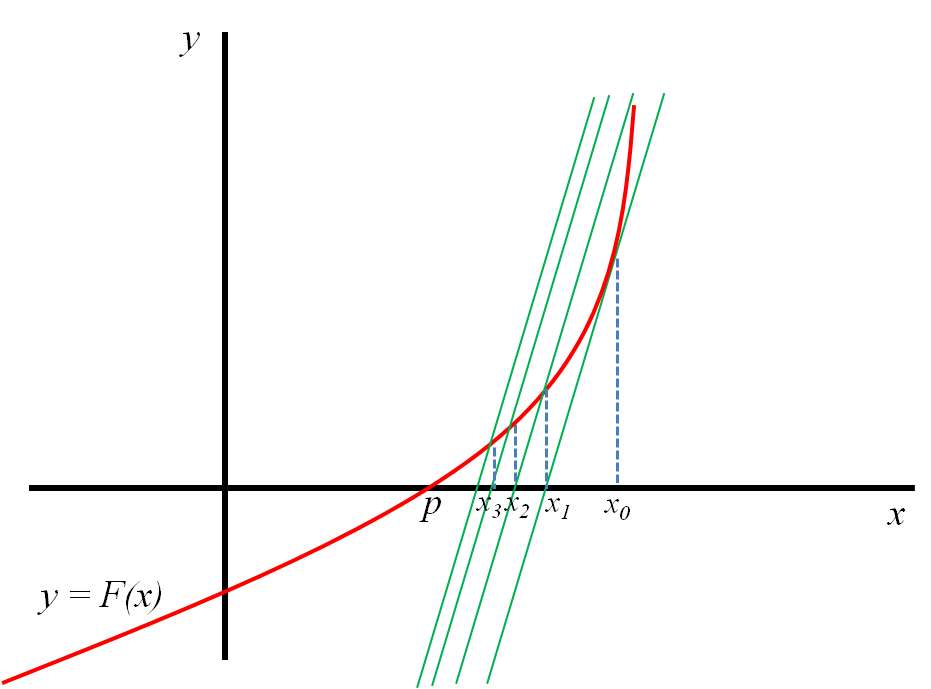
\includegraphics[width=0.75\linewidth]{Plots/U2/vonMises} \end{center}

\hypertarget{muxe9todo-de-newton-raphson-de-2uxba-orden}{%
\section{Método de Newton-Raphson de 2º Orden}\label{muxe9todo-de-newton-raphson-de-2uxba-orden}}

\begin{itemize}
\tightlist
\item
  Otra modificación al método de N-R se deriva a partir de la utilización de un término más en el desarrollo por serie de Taylor de la función \(F(x)\).
\item
  Dada la existencia de las correspondientes derivadas, la fórmula de recurrencia resultante es:
\end{itemize}

\[
x_k = x_{k-1} + \frac{F(x_{k-1})F'(x_{k-1})}{0.5 F(x_{k-1}) F''(x_{k-1}) - [F'(x_{k-1})]^2} \quad k = 1, 2, \dots
\]

\begin{itemize}
\tightlist
\item
  El método de N-R de 2º orden llega más rápidamente a la raíz, aunque la fórmula es más difícil de obtener.
\end{itemize}

\hypertarget{soluciuxf3n-de-sistemas-de-ecuaciones-lineales}{%
\chapter{Solución de Sistemas de Ecuaciones Lineales}\label{soluciuxf3n-de-sistemas-de-ecuaciones-lineales}}

\hypertarget{generalidades-1}{%
\section{Generalidades}\label{generalidades-1}}

\begin{itemize}
\tightlist
\item
  \textbf{Objetivo}: examinar los aspectos numéricos que se presentan al resolver sistemas de ecuaciones lineales de la forma:
\end{itemize}

\[
\begin{cases} 
a_{11}x_1 + a_{12}x_2 + \cdots + a_{1n}x_n = b_1 \\
a_{21}x_1 + a_{22}x_2 + \cdots + a_{2n}x_n = b_2 \\
\vdots \\
a_{n1}x_1 + a_{n2}x_2 + \cdots + a_{nn}x_n = b_n
\end{cases}
\]

\begin{itemize}
\tightlist
\item
  \(n\) ecuaciones, \(n\) incógnitas: sistema de orden \(n \times n\).
\item
  Los coeficientes \(a_{ij}\) y los términos independientes \(b_i\) son reales fijos.
\end{itemize}

\hypertarget{repaso}{%
\section{Repaso}\label{repaso}}

\begin{itemize}
\tightlist
\item
  Representación matricial: \(\mathbf{Ax=b}\), de dimensión \(n\times n\), \(n\times 1\) y \(n\times 1\), respectivamente.
\end{itemize}

\[
\begin{bmatrix}
a_{11} & a_{12} & \cdots & a_{1n} \\
a_{21} & a_{22} & \cdots & a_{2n} \\
\vdots & \vdots & \ddots & \vdots \\
a_{n1} & a_{n2} & \cdots & a_{nn} 
\end{bmatrix}
\times 
\begin{bmatrix}
x_1 \\ x_2 \\ \vdots \\ x_n
\end{bmatrix}
=
\begin{bmatrix}
b_1 \\ b_2 \\ \vdots \\ b_n
\end{bmatrix}
\]

\begin{itemize}
\tightlist
\item
  Llamamos \textbf{matriz ampliada} o \textbf{aumentada} a:
\end{itemize}

\[
\begin{bmatrix}
    \mathbf{A} & \mathbf{b}
\end{bmatrix}
=
\begin{bmatrix}
a_{11} & a_{12} & \cdots & a_{1n} & b_1\\
a_{21} & a_{22} & \cdots & a_{2n} & b_2\\
\vdots & \vdots & \ddots & \vdots & \vdots\\
a_{n1} & a_{n2} & \cdots & a_{nn} & b_n 
\end{bmatrix}
\]

\begin{itemize}
\item
  Un sistema de ecuaciones lineales se clasifica en:

  \begin{itemize}
  \tightlist
  \item
    \textbf{Compatible determinado}: tiene una única solución
  \item
    \textbf{Compatible indeterminado}: tiene infinitas soluciones
  \item
    \textbf{Incompatible}: no existe solución
  \end{itemize}
\end{itemize}

\begin{itemize}
\item
  \textbf{Teorema}. Las siguientes condiciones son equivalentes:

  \begin{itemize}
  \tightlist
  \item
    El sistema \(\mathbf{Ax=b}\) tiene solución única (es compatible determinado).
  \item
    La matriz \(\mathbf{A}\) es invertible (existe \(\mathbf{A^{-1}}\)).
  \item
    La matriz \(\mathbf{A}\) es no singular (\(\det \mathbf{A} \neq 0\)).
  \item
    El sistema \(\mathbf{Ax=0}\) tiene como única solución \(\mathbf{x=0}\).
  \end{itemize}
\item
  Dos sistemas de orden \(n \times n\) son \textbf{equivalentes} si tienen el mismo conjunto de soluciones.
\item
  Existen ciertas transformaciones sobre las ecuaciones de un sistema que no cambian el conjunto de soluciones (producen un sistema equivalente):

  \begin{itemize}
  \tightlist
  \item
    \textbf{Intercambio}: el orden de las ecuaciones puede cambiarse.
  \item
    \textbf{Escalado}: multiplicar una ecuación por una constante no nula.
  \item
    \textbf{Sustitución}: una ecuación puede ser reemplazada por una combinación lineal de las ecuaciones del sistema (\emph{teorema fundamental de la equivalencia})
  \end{itemize}
\item
  Realizar estas transformaciones sobre las ecuaciones es equivalente a realizar las mismas operaciones sobre las filas de la matriz aumentada.
\end{itemize}

\hypertarget{notaciuxf3n}{%
\section{Notación}\label{notaciuxf3n}}

\begin{itemize}
\item
  En esta sección presentamos la notación utilizaremos para expresar algoritmos con operaciones matriciales, facilitando su traducción a IML o R.
\item
  Dada una matriz \(\mathbf{Z}\) de dimensión \(n \times m\), anotamos:

  \begin{itemize}
  \tightlist
  \item
    \(z_{ij} = \mathbf{Z}[i, j]\): elemento en la fila \(i\) y columna \(j\) de la matriz \(\mathbf{Z}\)
  \item
    \(\mathbf{Z}[i,]\): vector fila de dimensión \(1\times m\) constituido por la \(i\)-ésima fila de la matriz \(\mathbf{Z}\)
  \item
    \(\mathbf{Z}[,j]\): vector columna \(n\times 1\) constituido por la \(j\)-ésima columna de la matriz \(\mathbf{Z}\)
  \item
    \(\mathbf{Z}[i,k:l]\): matriz de dimensión \(1\times (l-k+1)\) constituida con los elementos \(z_{i,k}, z_{i,k+1}, \cdots, z_{i,l}\) de la matriz \(\mathbf{Z}\), \(l \geq k\).
  \item
    \(\mathbf{Z}[c:d,k:l]\): matriz de dimensión \((d-c+1)\times (l-k+1)\) constituida por la submatriz que contiene las filas de \(\mathbf{Z}\) desde la \(c\) hasta \(d\) y las columnas de \(\mathbf{Z}\) desde la \(k\) hasta la \(l\), \(d \geq c\), \(l \geq k\).
  \end{itemize}
\item
  Dado un vector \(\mathbf{Z}\) de largo \(n\), anotamos:

  \begin{itemize}
  \tightlist
  \item
    \(\mathbf{Z}[i]\): elemento \(i\)-ésimo del vector \(\mathbf{Z}\)
  \item
    \(\mathbf{Z}[k:l]\): vector de largo \((l-k+1)\) constituido con los elementos \(z_{k}, z_{k+1}, \cdots, z_{l}\) del vector \(\mathbf{Z}\), \(l \geq k\).
  \end{itemize}
\end{itemize}

\hypertarget{muxe9todos-de-resoluciuxf3n-de-sistemas-de-ecuaciones}{%
\section{Métodos de Resolución de Sistemas de Ecuaciones}\label{muxe9todos-de-resoluciuxf3n-de-sistemas-de-ecuaciones}}

\begin{itemize}
\item
  \textbf{Métodos exactos}: permiten obtener la solución del sistema de manera directa.

  \begin{itemize}
  \tightlist
  \item
    Método de Eliminación de Gauss
  \item
    Método de Gauss-Jordan
  \end{itemize}
\item
  \textbf{Métodos aproximados}: utilizan algoritmos iterativos que calculan las solución del sistema por aproximaciones sucesivas.

  \begin{itemize}
  \tightlist
  \item
    Método de Jacobi
  \item
    Método de Gauss-Seidel
  \end{itemize}
\item
  En muchas ocasiones los métodos aproximados permiten obtener un grado de exactitud superior al que se puede obtener empleando los denominados métodos exactos, debido fundamentalmente a los errores de truncamiento que se producen en el proceso.
\end{itemize}

\hypertarget{muxe9todos-exactos}{%
\section{Métodos exactos}\label{muxe9todos-exactos}}

En esta sección repasaremos los métodos que ya conocen y que han aplicado ``a mano'' muchas veces para resolver sistemas de ecuaciones, con la particularidad de que pensaremos cómo expresar sus algoritmos para poder programarlos en la computadora. Entre los aspectos que tendremos que considerar, se encuentra la necesidad de aplicar estrategias de pivoteo (para evitar un \emph{pivote} igual a cero cuando se resuelve el sistema) y la posibilidad de realizar reordenamientos de la matriz de coeficientes para disminuir los errores producidos en los cálculos computacionales.

\hypertarget{sistemas-fuxe1ciles-de-resolver}{%
\subsection{Sistemas fáciles de resolver}\label{sistemas-fuxe1ciles-de-resolver}}

\textbf{Caso 1: La matriz} \(\mathbf{A}\) \textbf{es diagonal}

\[
\begin{bmatrix}
a_{11} & 0 & \cdots & 0 \\
0 & a_{22} & \cdots & 0 \\
\vdots & \vdots & \ddots & \vdots \\
0 & 0 & \cdots & a_{nn} 
\end{bmatrix}
\times 
\begin{bmatrix}
x_1 \\ x_2 \\ \vdots \\ x_n
\end{bmatrix}
=
\begin{bmatrix}
b_1 \\ b_2 \\ \vdots \\ b_n
\end{bmatrix}
\]

\begin{itemize}
\tightlist
\item
  El sistema se reduce a \(n\) ecuaciones simples y la solución es:
\end{itemize}

\[
\mathbf{x} =
\begin{bmatrix}
    b_1/a_{11} \\ b_2/a_{22} \\ \vdots \\ b_n/a_{nn}
\end{bmatrix}
\]

\textbf{Caso 2: La matrix} \(\mathbf{A}\) \textbf{es triangular superior}:

\[
\begin{bmatrix}
a_{11} & a_{12} & a_{13} & \cdots & a_{1n} \\
0 & a_{22} & a_{23} & \cdots & a_{2n} \\
0 & 0 & a_{33} & \cdots & a_{3n} \\
\vdots & \vdots & \vdots & \ddots & \vdots \\
0 & 0 & 0 & \cdots & a_{nn}
\end{bmatrix}
\times 
\begin{bmatrix}
x_1 \\ x_2 \\ \vdots \\ x_n
\end{bmatrix}
=
\begin{bmatrix}
b_1 \\ b_2 \\ \vdots \\ b_n
\end{bmatrix}
\]

\begin{itemize}
\tightlist
\item
  La solución de \(x_n\) es inmediata y a partir de ella se encuentran las restantes en orden inverso \(x_{n-1}, \cdots, x_1\), aplicando el algoritmo de \textbf{sustitución regresiva}:
\end{itemize}

\[
x_n = \frac{b_n}{a_{nn}} \text{ y } x_k = \frac{b_k - \sum_{j = k+1}^{n}a_{kj}x_j}{a_{kk}} \quad k = n-1, n-2, \cdots, 1
\]

\begin{itemize}
\tightlist
\item
  Empleando la notación matricial vista, la suma en el algoritmo puede reescribirse con productos matriciales:
\end{itemize}

\[
\mathbf{x}[n] = \frac{\mathbf{b}[n]}{\mathbf{A}[n,n]} \qquad \mathbf{x}[k] = \frac{\mathbf{b}[k] - \mathbf{A}[k, k+1 : n] \times \mathbf{x}[k+1 : n]}{\mathbf{A}[k,k]}
\]
\[
\quad k = n-1, n-2, \cdots, 1
\]

\begin{itemize}
\tightlist
\item
  Iniciando el vector solución con ceros, \(\mathbf{x} = [0 ~ 0 \cdots 0]\), la expresión anterior se simplifica como:
\end{itemize}

\[
\mathbf{x}[n] = \frac{\mathbf{b}[n]}{\mathbf{A}[n,n]} \qquad \mathbf{x}[k] = \frac{\mathbf{b}[k] - \mathbf{A}[k, ] \times \mathbf{x}}{\mathbf{A}[k,k]}
\qquad k = n-1, n-2, \cdots, 1
\]

\textbf{Tarea:} ver el algoritmo en documento adjunto y programarlo.

\textbf{Caso 3: La matrix} \(\mathbf{A}\) \textbf{es triangular inferior}:

\begin{itemize}
\tightlist
\item
  Obtención de la solución análoga al caso anterior.
\end{itemize}

\textbf{Observaciones}

\begin{itemize}
\tightlist
\item
  En los casos anteriores asumimos \(a_{kk} \neq 0 \quad \forall \quad k\). De lo contrario el sistema no tiene solución o tiene infinitas.
\item
  Recordar que un sistema lineal \(\mathbf{Ax=b}\) tiene solución única si y sólo si \(\det \mathbf{A} \neq 0\) y que si un elemento de la diagonal principal de una matriz triangular es cero, entonces \(\det \mathbf{A} = 0\).
\end{itemize}

\hypertarget{eliminaciuxf3n-gaussiana}{%
\subsection{Eliminación gaussiana}\label{eliminaciuxf3n-gaussiana}}

\begin{itemize}
\tightlist
\item
  Es un método para resolver un sistema lineal general \(\mathbf{Ax=b}\) de \(n\) ecuaciones con \(n\) incógnitas.
\item
  El objetivo es construir un sistema equivalente donde la matriz de coeficientes sea triangular superior para obtener las soluciones con el algoritmo de sustitución regresiva.
\item
  El método consiste en ir eliminando incógnitas en las ecuaciones de manera sucesiva.
\item
  Ejemplo: resolver el siguiente sistema
\end{itemize}

\[
\begin{cases} 
x+2y-z+3t=-8 \\
2x+2z-t=13 \\
-x+y+z-t=8\\
3x+3y-z+2t = -1
\end{cases}
\mathbf{A}=
\begin{bmatrix}
1 & 2 & -1 & 3 \\
2 & 0 & 2 & -1 \\
-1 & 1 & 1 & -1 \\
3 & 3 & -1 & 2 &  
\end{bmatrix}
\mathbf{x} = 
\begin{bmatrix}
x \\ y \\ z \\ t
\end{bmatrix}
\mathbf{b} =
\begin{bmatrix}
-8 \\ 13 \\ 8 \\ -1
\end{bmatrix}
\]

\begin{itemize}
\tightlist
\item
  Matriz aumentada:
\end{itemize}

\[
\begin{bmatrix}
    \mathbf{A} & \mathbf{b}
\end{bmatrix}
=
\begin{bmatrix}
    1 & 2 & -1 & 3 &|& -8\\
    2 & 0 & 2 & -1 &|& 13\\
    -1 & 1 & 1 & -1 &|& 8\\
    3 & 3 & -1 & 2 &|& -1  
\end{bmatrix}
\]

\begin{itemize}
\tightlist
\item
  En el primer paso eliminamos la incógnita \(x\) en las ecuaciones 2, 3 y 4, buscando que queden ceros en toda la primera columna excepto en el elemento diagonal.
\item
  La eliminación se hace empleando las transformaciones que producen un sistema equivalente.
\item
  Observando con detenimiento, esto se puede lograr realizando los siguientes reemplazos:
\end{itemize}

\[
\begin{array}{cl}
\text{Fila 2} &= \text{ Fila 2} - 2 \times \text{Fila 1} \\ 
\text{Fila 3} &= \text{ Fila 3} - (-1) \times \text{Fila 1} \\
\text{Fila 4} &= \text{ Fila 4} - 3 \times \text{Fila 1} 
\end{array}
\]

\begin{itemize}
\tightlist
\item
  A la Fila 1 se le dice \textbf{fila pivote} y al elemento \(a_{11}=1\), \textbf{pivote}. A los valores \(2\), \(-1\) y \(3\) que multiplican a la fila pivote en los reemplazos se les dice \textbf{multiplicadores}.
\item
  De manera general, los multiplicadores se simbolizan y obtienen con:
\end{itemize}

\[m_{r1} = a_{r1} / a_{11}, \quad r = 2, 3, ..., n\]

\begin{itemize}
\tightlist
\item
  De esta forma, los reemplazos realizados se generalizan como:
\end{itemize}

\[\text{Fila } r = \text{Fila } r - m_{r1} \times \text{Fila 1}\]
- El resultado de los reemplazos anteriores es:

\[
\begin{matrix}
\text{pivote} \rightarrow \\ m_{21} = 2 \\ m_{31} = -1 \\ m_{41} = 3
\end{matrix}
\begin{bmatrix}
1 & 2 & -1 & 3 &|& -8\\
2 & 0 & 2 & -1 &|& 13\\
-1 & 1 & 1 & -1 &|& 8\\
3 & 3 & -1 & 2 &|& -1  
\end{bmatrix}
\implies
\begin{bmatrix}
1 & 2 & -1 & 3 &|& -8\\
0 & -4 & 4 & -7 &|& 29\\
0 & 3 & 0 & 2 &|& 0\\
0 & -3 & 2 & -7 &|& 23  
\end{bmatrix}
\]

\begin{itemize}
\tightlist
\item
  En el segundo paso, eliminamos la incógnita \(y\) en las ecuaciones 3 y 4. La fila pivote pasa a ser la segunda y el pivote es \(a_{22}=-4\). Los multiplicadores son \(m_{r2}=a_{r2}/a_{22}\), \(r=3,4\), dando lugar a los reemplazos:
\end{itemize}

\[
\begin{array}{cl}
\text{Fila 3} &= \text{ Fila 3} - (-3/4) \times \text{Fila 2} \\
\text{Fila 4} &= \text{ Fila 4} - 3/4 \times \text{Fila 2} 
\end{array}
\]

\begin{itemize}
\tightlist
\item
  El resultado es:
\end{itemize}

\[
\begin{matrix}
 \\ \text{pivote} \rightarrow \\ m_{32} = -3/4 \\ m_{42} = 3/4
\end{matrix}
\begin{bmatrix}
1 & 2 & -1 & 3 &|& -8\\
0 & -4 & 4 & -7 &|& 29\\
0 & 3 & 0 & 2 &|& 0\\
0 & -3 & 2 & -7 &|& 23  
\end{bmatrix}
\implies
\]

\[
\begin{bmatrix}
1 & 2 & -1 & 3 &|& -8\\
0 & -4 & 4 & -7 &|& 29\\
0 & 0 & -12 & 13 &|& -87\\
0 & 0 & 4 & 7 &|& -5  
\end{bmatrix}
\]

\begin{itemize}
\tightlist
\item
  Finalmente, eliminamos la incógnita \(z\) en la última ecuación. La fila pivote es la 3º y el pivote es \(a_{33}=-12\). El multiplicador es \(m_{43}=a_{43}/a_{33}=-4/12\).
\item
  El reemplazo a realizar es:
\end{itemize}

\[\text{Fila } 4 = \text{Fila } 4 - (-4/12) \times \text{Fila } 3\]

\begin{itemize}
\tightlist
\item
  El resultado es:
\end{itemize}

\[
\begin{matrix}
\\ \\ \text{pivote} \rightarrow \\ m_{43} = -4/12
\end{matrix}
\begin{bmatrix}
1 & 2 & -1 & 3 &|& -8\\
0 & -4 & 4 & -7 &|& 29\\
0 & 0 & -12 & 13 &|& -87\\
0 & 0 & 4 & 7 &|& -5  
\end{bmatrix}
\implies
\]

\[
\begin{bmatrix}
1 & 2 & -1 & 3 &|& -8\\
0 & -4 & 4 & -7 &|& 29\\
0 & 0 & -12 & 13 &|& -87\\
0 & 0 & 0 & -136 &|& 408  
\end{bmatrix}
\]

\begin{itemize}
\tightlist
\item
  Hemos llegado a un sistema equivalente cuya matriz de coeficientes es triangular superior, en el que aplicamos el algoritmo de sustitución regresiva:
\end{itemize}

\[
\left\{
\begin{aligned}
x+2y-z-3t &=-8 \cr
-4y+4z-7t &=29\cr
-12z+13t &=-87\cr
-136t &=408
\end{aligned}
\right.
\implies
\left\{
\begin{aligned}
x &= 1\\ y &= 2\\ z &= 4\\ t &= -3
\end{aligned}
\right.
\]

\textbf{Tarea:} revisar el algoritmo y la función ya programada.

\hypertarget{eliminaciuxf3n-gaussiana-con-pivoteo-trivial}{%
\subsubsection*{Eliminación gaussiana con pivoteo trivial}\label{eliminaciuxf3n-gaussiana-con-pivoteo-trivial}}
\addcontentsline{toc}{subsubsection}{Eliminación gaussiana con pivoteo trivial}

\begin{itemize}
\tightlist
\item
  En el algoritmo anterior es necesario que los pivotes \(a_{qq} \neq 0 ~\forall q\).
\item
  Si en uno de los pasos encontramos un \(a_{qq} = 0\), debemos intercambiar la \(q\)-ésima fila por una cualquiera de las siguientes, por ejemplo la fila \(k\), en la que \(a_{kq} \neq 0, k>q\).
\item
  Esta estrategia para hallar un pivote no nulo se llama \textbf{pivoteo trivial}.
\item
  \textbf{Tarea:} verificar ``a mano'' que con el siguiente sistema, si seguimos el algoritmo anterior, incurrimos en este problema. En cambio, si seguimos el algoritmo con pivoteo trivial (ver en documento adjunto y su programa) no tenemos dicho problema.
\end{itemize}

\[
\begin{cases} 
x-2y+z=-4 \\
-2x+4y-3z=3 \\
x-3y-4z=-1
\end{cases}
\]

\hypertarget{estrategias-de-pivoteo-para-reducir-los-errores}{%
\subsection{Estrategias de pivoteo para reducir los errores}\label{estrategias-de-pivoteo-para-reducir-los-errores}}

\begin{itemize}
\tightlist
\item
  Como ya sabemos, dado que las computadoras usan una aritmética cuya precisión está fijada de antemano, es posible que cada vez que se realice una operación aritmética se introduzca un pequeño error.
\item
  En la resolución de ecuaciones por eliminación gaussiana, un adecuado reordenamiento de las filas en el momento indicado puede reducir notablemente los errores cometidos.
\item
  Por ejemplo, se puede mostrar cómo buscar un multiplicador de menor magnitud (es decir, un pivote de mayor magnitud) mejora la precisión de los resultados.
\item
  Por eso, existen estrategias de pivoteo que no solamente hacen intercambio de filas cuando se tiene un pivote nulo, si no también cuando alguna de las filas posteriores tiene un pivote de mayor valor absoluto.
\end{itemize}

\hypertarget{pivoteo-parcial}{%
\subsubsection*{Pivoteo parcial}\label{pivoteo-parcial}}
\addcontentsline{toc}{subsubsection}{Pivoteo parcial}

\begin{itemize}
\tightlist
\item
  Para reducir la propagación de los errores de redondeo, antes de comenzar una nueva ronda de reemplazos con el pivote \(a_{qq}\) se evalúa si debajo en la misma columna hay algún elemento con mayor valor absoluto y en ese caso se intercambian las respectivas filas.
\item
  Es decir, se busca si existe \(r\) tal que \(|a_{rq}| > |a_{qq}|,\quad r>q\) para luego intercambiar las filas \(q\) y \(r\).
\item
  Este proceso suele conservar las magnitudes relativas de los elementos de la matriz triangular superior en el mismo orden que las de los coeficientes de la matriz original.
\item
  \textbf{Tarea}: leer el algoritmo del pivoteo parcial en el documento adjunto y programarlo.
\end{itemize}

\hypertarget{pivoteo-parcial-escalado}{%
\subsubsection*{Pivoteo parcial escalado}\label{pivoteo-parcial-escalado}}
\addcontentsline{toc}{subsubsection}{Pivoteo parcial escalado}

\begin{itemize}
\tightlist
\item
  Reduce aún más los efectos de la propagación de los errores.
\item
  Se elige el elemento de la columna \(q\)-ésima, en o por debajo de la diagonal principal, que tiene mayor tamaño relativo con respecto al resto de los elementos de su fila.
\item
  \textbf{Paso 1}: buscar el máximo valor absoluto en cada fila:
\end{itemize}

\[
s_r = max\{|a_{rq}|, |a_{r,q+1}|, \cdots, |a_{rn}| \} \quad r = q, q+1, \cdots, n
\]

\begin{itemize}
\tightlist
\item
  \textbf{Paso 2}: elegir como fila pivote a la que tenga el mayor valor de \(\frac{|a_{rq}|}{s_r}\), \(r = q, q+1, \cdots, n\).
\item
  \textbf{Paso 3}: intercambiar la fila \(q\) con la fila hallada en el paso 2.
\item
  \textbf{Tarea}: leer el algoritmo del pivoteo parcial en el documento adjunto y programarlo.
\end{itemize}

\hypertarget{muxe9todo-de-eliminaciuxf3n-de-gauss-jordan}{%
\subsection{Método de eliminación de Gauss-Jordan}\label{muxe9todo-de-eliminaciuxf3n-de-gauss-jordan}}

\begin{itemize}
\tightlist
\item
  Ya vimos que el método de Gauss transforma la matriz de coeficientes en una matriz triangular superior.
\item
  El método de Gauss-Jordan continúa el proceso de transformación hasta obtener la matriz identidad.
\item
  En el ejemplo de la sección 3.6, cuando aplicamos eliminación de Gauss habíamos llegado a la siguiente matriz triangular:
\end{itemize}

\[
\begin{bmatrix}
1 & 2 & -1 & 3 &|& -8\\
0 & -4 & 4 & -7 &|& 29\\
0 & 0 & -12 & 13 &|& -87\\
0 & 0 & 0 & -136 &|& 408  
\end{bmatrix}
\]

\begin{itemize}
\tightlist
\item
  Luego, con el método de sustitución regresiva, llegamos a encontrar \(x=1\), \(y=2\), \(z=4\) y \(t=-3\).
\item
  En lugar de aplicar sustitución regresiva, seguimos operando por fila hasta lograr una matriz diagonal:
\end{itemize}

\[
\begin{array}{cl}
\text{Fila 2} &= \text{ Fila 2} / (-4) \\ 
\text{Fila 3} &= \text{ Fila 3} /(-12) \\
\text{Fila 4} &= \text{ Fila 4} / (-136) 
\end{array}
\implies
\begin{bmatrix}
1 & 2 & -1 & 3 &|& -8\\
0 & 1 & -1 & 7/4 &|& -29/4\\
0 & 0 & 1 & -13/12 &|& 87/12\\
0 & 0 & 0 & 1 &|& -3  
\end{bmatrix}
\]

\[
\begin{array}{cl}
\text{Fila 1} &= \text{ Fila 1} - 3 \text{ Fila 4} \\ 
\text{Fila 2} &= \text{ Fila 2} - 7/4 \text{ Fila 4}\\
\text{Fila 3} &= \text{ Fila 3} + 13/12 \text{ Fila 4} 
\end{array}
\implies
\begin{bmatrix}
1 & 2 & -1 & 0 &|& 1\\
0 & 1 & -1 & 0 &|& -2\\
0 & 0 & 1 & 0 &|& 4\\
0 & 0 & 0 & 1 &|& -3  
\end{bmatrix}
\]

\[
\begin{array}{cl}
\text{Fila 1} &= \text{ Fila 1} + \text{ Fila 3} \\ 
\text{Fila 2} &= \text{ Fila 2} + \text{ Fila 3}
\end{array}
\implies
\begin{bmatrix}
1 & 2 & 0 & 0 &|& 5\\
0 & 1 & 0 & 0 &|& 2\\
0 & 0 & 1 & 0 &|& 4\\
0 & 0 & 0 & 1 &|& -3  
\end{bmatrix}
\]

\[
\begin{array}{cl}
\text{Fila 1} &= \text{ Fila 1} -2 \text{ Fila 2} 
\end{array}
\implies
\begin{bmatrix}
1 & 0 & 0 & 0 &|& 1\\
0 & 1 & 0 & 0 &|& 2\\
0 & 0 & 1 & 0 &|& 4\\
0 & 0 & 0 & 1 &|& -3  
\end{bmatrix}
\]

\[
\implies
\left\{
\begin{aligned}
x &= 1\\ y &= 2\\ z &= 4\\ t &= -3
\end{aligned}
\right.
\]

\begin{itemize}
\tightlist
\item
  La ventaja de este método es que permite también hallar fácilmente la matriz inversa de \(\mathbf{A}\).
\item
  Para esto hay que concatenar a la derecha de la matriz aumentada una matriz identidad de orden \(n\). Cuando en la submatriz izquierda se llega a la matriz identidad, en el centro habrá quedado el vector solución y a su derecha la matriz inversa.
\item
  \textbf{Ejemplo}. Resolver el siguiente sistema y hallar la inversa de la matriz de coeficientes:
\end{itemize}

\[
\begin{cases} 
x-y+z=-4 \\
5x-4y+3z=-12 \\
2x+y+z=11
\end{cases}
\]

\[
\begin{bmatrix}
    1 & -1 & 1 &|& -4 &|& 1 & 0 & 0\\
    5 & -4 & 3 &|& -12 &|& 0 & 1 & 0\\
    2 & 1 & 1 &|& 11 &|& 0 & 0 & 1
\end{bmatrix}
\]

\[
\begin{array}{cl}
    F2 &= F2 - 5 F1 \\
    F3 &= F3 - 2 F1 \\
    F1 &= F1 + F2 \\
    F3 &= F3 - 3 F2 \\
    F1 &= F1 + 1/5 F3 \\
    F2 &= F2 + 2/5 F3  \\
    F3 &= F3 / 5
\end{array}
\]

\[
\begin{bmatrix}
    1 & 0 & 0 &|& 3 &|& -7/5 & 2/5 & 1/5\\
    0 & 1 & 0 &|& 6 &|& 1/5 & -1/5 & 2/5\\
    0 & 0 & 1 &|& -1 &|& 13/5 & -3/2 & 1/5
\end{bmatrix}
\]

\begin{itemize}
\item
  ¿Por qué este procedimiento nos devuelva la inversa de la matriz de coeficientes?
\item
  Recordar que la inversa de \(\mathbf{A}\) es aquella matriz \(\mathbf{A}^{-1}\) que verifica \(\mathbf{AA}^{-1} =\mathbf{A}^{-1}\mathbf{A}=\mathbf{I}\)
\item
  Entonces si queremos hallar la matriz \(\mathbf{A}^{-1}\):

  \[
    \mathbf{A}^{-1} =
    \begin{bmatrix}
    x_{11} & x_{12} & x_{13} \\
    x_{21} & x_{22} & x_{23} \\
    x_{31} & x_{32} & x_{33} 
    \end{bmatrix}
    \]

  podemos plantear el siguiente producto matricial:

  \[
    \begin{bmatrix}
    1 & -1 & 1 \\
    5 & -4 & 3 \\
    2 & 1 & 1 
    \end{bmatrix}
    \times
    \begin{bmatrix}
    x_{11} & x_{12} & x_{13} \\
    x_{21} & x_{22} & x_{23} \\
    x_{31} & x_{32} & x_{33} 
    \end{bmatrix}
    =
    \begin{bmatrix}
    1 & 0 & 0 \\
    0 & 1 & 0 \\
    0 & 0 & 1 
    \end{bmatrix}
    \]

  que da lugar a tres sistemas de ecuaciones con la misma matriz de coeficientes:

  \[
    \implies
    \begin{bmatrix}
    x_{11}-x_{21}+x_{31} & x_{12}-x_{22}+x_{32} & x_{13}-x_{23}+x_{33} \\
    5x_{11}-4x_{21}+3x_{31} & 5x_{12}-4x_{22}+3x_{32} & 5x_{13}-4x_{23}+3x_{33} \\
    2x_{11}+x_{21}+x_{31} & 2x_{12}-x_{22}+x_{32} & 2x_{13}-x_{23}+x_{33} 
    \end{bmatrix}
    =
    \]

  \[
    =
    \begin{bmatrix}
    1 & 0 & 0 \\
    0 & 1 & 0 \\
    0 & 0 & 1 
    \end{bmatrix}
    \]

  \[
    \begin{cases} 
    x_{11}-x_{21}+x_{31}=1 \\
    5x_{11}-4x_{21}+3x_{31}=0 \\
    2x_{11}+x_{21}+x_{31}=0
    \end{cases}
    \]

  \[
    \begin{cases} 
    x_{12}-x_{22}+x_{32}=0 \\
    5x_{12}-4x_{22}+3x_{32}=1 \\
    2x_{12}+x_{22}+x_{32}=0
    \end{cases}
    \]

  \[
    \begin{cases} 
    x_{13}-x_{23}+x_{33}=0 \\
    5x_{13}-4x_{23}+3x_{33}=0 \\
    2x_{13}+x_{23}+x_{33}=1
    \end{cases}
    \]
\item
  Los resolvemos simultáneamente al agregarle a la matriz aumentada del sistema original, estos tres ``nuevos vectores de términos independientes'' que forman una matriz identidad de orden \(n\). En cierto modo, estamos resolviendo cuatro sistemas de ecuaciones a la vez, el sistema original y los tres que permiten hallar cada columna de \(\mathbf{A}^{-1}\).
\item
  \textbf{Tarea}. Revisar el algoritmo y programarlo.
\end{itemize}

\hypertarget{muxe9todos-aproximados-o-iterativos}{%
\section{Métodos Aproximados o Iterativos}\label{muxe9todos-aproximados-o-iterativos}}

\begin{itemize}
\item
  \textbf{Objetivo}: extender a espacios de dimensión mayor que 1 las ideas de los métodos iterativos vistos en la Unidad 2 para resolver sistemas de ecuaciones lineales.
\item
  Veremos:

  \begin{itemize}
  \tightlist
  \item
    Método de Jacobi
  \item
    Método de Gauss-Seidel
  \end{itemize}
\end{itemize}

\hypertarget{muxe9todo-de-jacobi}{%
\subsection{Método de Jacobi}\label{muxe9todo-de-jacobi}}

\begin{itemize}
\tightlist
\item
  Consideremos el sistema:
\end{itemize}

\[
\begin{cases} 
4x-y+z=7 \\
4x-8y+z=-21 \\
-2x+y+5z=15
\end{cases}
\implies
\begin{cases} 
x=(7+y-z)/4 \\
y=(21+4x+z)/8 \\
z=(15+2x-y)/5
\end{cases}
\]

\begin{itemize}
\tightlist
\item
  Despejar una incógnita en cada ecuación provee expresiones que sugieren la idea de un proceso iterativo.
\item
  Dado un vector de valores iniciales \(\mathbf{x_0}=(x_0, y_0, z_0)\), operar con la siguiente fórmula de recurrencia hasta la convergencia:
\end{itemize}

\[
\begin{cases} 
x_{k+1}=(7+y_k-z_k)/4 \\
y_{k+1}=(21+4x_k+z_k)/8 \\
z_{k+1}=(15+2x_k-y_k)/5
\end{cases}
\]

\begin{itemize}
\tightlist
\item
  Por ejemplo, tomando el valor inicial \((1, 2, 2)\), el proceso converge hacia la solución exacta del sistema \((2, 4, 3)\).
\item
  Usando 4 posiciones decimales con redondeo luego de la coma:
\end{itemize}

\begin{longtable}[]{@{}llll@{}}
\toprule
\(k\) & \(x_k\) & \(y_k\) & \(z_k\)\tabularnewline
\midrule
\endhead
0 & 1 & 2 & 2\tabularnewline
1 & 1.7500 & 3.3750 & 3.0000\tabularnewline
2 & 1.8438 & 3.8750 & 3.0250\tabularnewline
3 & 1.9625 & 3.9250 & 2.9625\tabularnewline
4 & 1.9906 & 3.9766 & 3.0000\tabularnewline
5 & 1.9942 & 3.9953 & 3.0009\tabularnewline
6 & 1.9986 & 3.9972 & 2.9986\tabularnewline
7 & 1.9997 & 3.9991 & 3.0000\tabularnewline
8 & 1.9998 & 3.9999 & 3.0001\tabularnewline
9 & 2.0000 & 3.9999 & 2.9999\tabularnewline
10 & 2.0000 & 4.0000 & 3.0000\tabularnewline
\bottomrule
\end{longtable}

\begin{itemize}
\tightlist
\item
  \emph{Observación}: no siempre este método converge. Es sensible al ordenamiento de las ecuaciones dentro del sistema.
\item
  Ejemplo: tomamos el mismo sistema de antes pero intercambiamos las filas 1 y 3:
\end{itemize}

\[
\begin{cases} 
4x-y+z=7 \\
4x-8y+z=-21 \\
-2x+y+5z=15
\end{cases}
\implies
\begin{cases} 
-2x+y+5z=15 \\
4x-8y+z=-21 \\
4x-y+z=7
\end{cases}
\]

\[
\implies
\begin{cases} 
x=(-15+y+5z)/2 \\
y=(21+4x+z)/8 \\
z=7-4x+y
\end{cases}
\implies
\begin{cases} 
x_{k+1}=(-15+y_k+5z_k)/2 \\
y_{k+1}=(21+4x_k+z_k)/8 \\
z_{k+1}=7-4x_k+y_k
\end{cases}
\]

\begin{itemize}
\tightlist
\item
  Tomando el mismo valor inicial \((1, 2, 2)\), esta vez el proceso diverge:
\end{itemize}

\begin{longtable}[]{@{}llll@{}}
\toprule
\(k\) & \(x_k\) & \(y_k\) & \(z_k\)\tabularnewline
\midrule
\endhead
0 & 1 & 2 & 2\tabularnewline
1 & -1.5000 & 3.3750 & 5.0000\tabularnewline
2 & 6.6875 & 2.5000 & 16.3750\tabularnewline
3 & 34.6875 & 8.0156 & -17.2500\tabularnewline
4 & -46.6172 & 17.8125 & -123.7344\tabularnewline
5 & -307.9298 & -36.1504 & 211.2813\tabularnewline
6 & 502.6281 & -124.9297 & 1202.5688\tabularnewline
7 & 2936.4572 & 404.2602 & -2128.4421\tabularnewline
8 & -5126.4752 & 1204.7983 & -11334.5686\tabularnewline
9 & -27741.5224 & -3977.4337 & 21717.6991\tabularnewline
10 & 52298.0309 & -11153.4238 & 106995.6559\tabularnewline
\bottomrule
\end{longtable}

\hypertarget{muxe9todo-de-gauss-seidel}{%
\subsection{Método de Gauss-Seidel}\label{muxe9todo-de-gauss-seidel}}

\begin{itemize}
\tightlist
\item
  Toma la misma idea que Jacobi, pero con una pequeña modificación para acelerar la convergencia. Retomando el ejemplo inicial:
\end{itemize}

\[
\begin{cases} 
4x-y+z=7 \\
4x-8y+z=-21 \\
-2x+y+5z=15
\end{cases}
\implies
\begin{cases} 
x=(7+y-z)/4 \\
y=(21+4x+z)/8 \\
z=(15+2x-y)/5
\end{cases}
\]

Jacobi:

\[
\begin{cases} 
x_{k+1}=(7+y_k-z_k)/4 \\
y_{k+1}=(21+4x_k+z_k)/8 \\
z_{k+1}=(15+2x_k-y_k)/5
\end{cases}
\]

Gauss-Seidel:

\[
\begin{cases} 
x_{k+1}=(7+y_k-z_k)/4 \\
y_{k+1}=(21+4x_{k+1}+z_k)/8 \\
z_{k+1}=(15+2x_{k+1}-y_{k+1})/5
\end{cases}
\]

\begin{itemize}
\item
  La diferencia está en que apenas calcula un nuevo valor de las incógnitas, Gauss-Seidel lo usa inmediatamente en el cálculo de las restantes, en lugar esperar a la próxima ronda.
\item
  Tomando otra vez el valor inicial \((1, 2, 2)\) y operando con 4 posiciones decimales con redondeo luego de la coma:
\end{itemize}

\begin{longtable}[]{@{}llllllll@{}}
\toprule
\textbf{Jacobi} & & & & \textbf{Gauss-Seidel} & & &\tabularnewline
\midrule
\endhead
\(k\) & \(x_k\) & \(y_k\) & \(z_k\) & \(k\) & \(x_k\) & \(y_k\) & \(z_k\)\tabularnewline
0 & 1 & 2 & 2 & 0 & 1 & 2 & 2\tabularnewline
1 & 1.7500 & 3.3750 & 3.0000 & 1 & 1.7500 & 3.7500 & 2.9500\tabularnewline
2 & 1.8438 & 3.8750 & 3.0250 & 2 & 1.9500 & 3.9688 & 2.9862\tabularnewline
3 & 1.9625 & 3.9250 & 2.9625 & 3 & 1.9957 & 3.9961 & 2.9991\tabularnewline
4 & 1.9906 & 3.9766 & 3.0000 & 4 & 1.9993 & 3.9995 & 2.9998\tabularnewline
5 & 1.9942 & 3.9953 & 3.0009 & 5 & 1.9999 & 3.9999 & 3.0000\tabularnewline
6 & 1.9986 & 3.9972 & 2.9986 & 6 & 2.0000 & 4.0000 & 3.0000\tabularnewline
7 & 1.9997 & 3.9991 & 3.0000 & & & &\tabularnewline
8 & 1.9998 & 3.9999 & 3.0001 & & & &\tabularnewline
9 & 2.0000 & 3.9999 & 2.9999 & & & &\tabularnewline
10 & 2.0000 & 4.0000 & 3.0000 & & & &\tabularnewline
& & & & & & &\tabularnewline
\bottomrule
\end{longtable}

\hypertarget{generalizaciuxf3n}{%
\subsection{Generalización}\label{generalizaciuxf3n}}

\begin{itemize}
\tightlist
\item
  Ahora que sabemos qué hace cada método y en qué se diferencian, vamos a generalizar las fórmulas recursivas.
\item
  Pensemos en un sistema de \(n\) ecuaciones lineales con \(n\) incógnitas y despejamos una variable en cada ecuación:
\end{itemize}

\[
\begin{cases} 
a_{11}x_1 + a_{12}x_2 + \cdots + a_{1n}x_n = b_1 \\
a_{21}x_1 + a_{22}x_2 + \cdots + a_{2n}x_n = b_2 \\
\vdots \\
a_{j1}x_1 + a_{j2}x_2 + \cdots + a_{jn}x_n = b_j \\
\vdots \\
a_{n1}x_1 + a_{n2}x_2 + \cdots + a_{nn}x_n = b_n
\end{cases}
\]
\[
\implies\hspace{-0.2cm}
\begin{cases} 
x_1 = \frac{b_1 - a_{12}x_2 - \cdots - a_{1n}x_n}{ a_{11}}\\
x_2 = \frac{b_2 - a_{21}x_1 - a_{23}x_3 - \cdots - a_{2n}x_n}{ a_{22}}\\
\vdots \\
x_j = \frac{b_j - a_{j1}x_1 \cdots - a_{j(j-1)}x_{j-1} - a_{j(j+1)}x_{j+1} - \cdots - a_{jn}x_n}{ a_{jj}}\\
\vdots \\
x_n = \frac{b_n - a_{n1}x_1 - \cdots - a_{n(n-1)}x_{n-1}}{a_{nn}}\\
\end{cases}
\]

\hypertarget{generalizaciuxf3n-del-muxe9todo-de-jacobi}{%
\subsubsection*{Generalización del Método de Jacobi}\label{generalizaciuxf3n-del-muxe9todo-de-jacobi}}
\addcontentsline{toc}{subsubsection}{Generalización del Método de Jacobi}

Con los supra índices indicando el número de iteración, la fórmula de recurrencia es:

\[
\begin{cases} 
x_1^{(k+1)} = \frac{b_1 - a_{12}x_2^{(k)} - \cdots - a_{1n}x_n^{(k)}}{ a_{11}}\\
x_2^{(k+1)} = \frac{b_2 - a_{21}x_1^{(k)} - a_{23}x_3^{(k)} - \cdots - a_{2n}x_n^{(k)}}{ a_{22}}\\
\vdots \\
x_j^{(k+1)} = \frac{b_j - a_{j1}x_1^{(k)} \cdots - a_{j(j-1)}x_{j-1}^{(k)} - a_{j(j+1)}x_{j+1}^{(k)} - \cdots - a_{jn}x_n^{(k)}}{ a_{jj}}\\
\vdots \\
x_n^{(k+1)} = \frac{b_n - a_{n1}x_1^{(k)} - \cdots - a_{n(n-1)}x_{n-1}^{(k)}}{a_{nn}}\\
\end{cases}
\]

\[
\implies
x_j^{(k+1)} = \frac{b_j - a_{j1}x_1^{(k)} \cdots - a_{j(j-1)}x_{j-1}^{(k)} - a_{j(j+1)}x_{j+1}^{(k)} - \cdots - a_{jn}x_n^{(k)}}{ a_{jj}}
\]
\[
k=1, 2, \cdots n
\]

\hypertarget{generalizaciuxf3n-del-muxe9todo-de-gauss-seidel}{%
\subsubsection*{Generalización del Método de Gauss-Seidel}\label{generalizaciuxf3n-del-muxe9todo-de-gauss-seidel}}
\addcontentsline{toc}{subsubsection}{Generalización del Método de Gauss-Seidel}

Con los supra índices indicando el número de iteración, la fórmula de recurrencia es:

\[
\begin{cases} 
x_1^{(k+1)} = \frac{b_1 - a_{12}x_2^{(k)} - \cdots - a_{1n}x_n^{(k)}}{ a_{11}}\\
x_2^{(k+1)} = \frac{b_2 - a_{21}x_1^{(k+1)} - a_{23}x_3^{(k)} - \cdots - a_{2n}x_n^{(k)}}{ a_{22}}\\
\vdots \\
x_j^{(k+1)} = \frac{b_j - a_{j1}x_1^{(k+1)} \cdots - a_{j(j-1)}x_{j-1}^{(k+1)} - a_{j(j+1)}x_{j+1}^{(k)} - \cdots - a_{jn}x_n^{(k)}}{ a_{jj}}\\
\vdots \\
x_n^{(k+1)} = \frac{b_n - a_{n1}x_1^{(k+1)} - \cdots - a_{n(n-1)}x_{n-1}^{(k+1)}}{a_{nn}}\\
\end{cases}
\]

\[
\implies
x_j^{(k+1)} = \frac{b_j - a_{j1}x_1^{(k+1)} \cdots - a_{j(j-1)}x_{j-1}^{(k+1)} - a_{j(j+1)}x_{j+1}^{(k)} - \cdots - a_{jn}x_n^{(k)}}{ a_{jj}}
\]
\[
k=1, 2, \cdots n
\]

\hypertarget{expresiuxf3n-matricial}{%
\subsection{Expresión matricial}\label{expresiuxf3n-matricial}}

\begin{itemize}
\tightlist
\item
  Ahora vamos a ver que es posible escribir las fórmulas recursivas anteriores de manera matricial, de modo que sea más fácil programar estos métodos.
\item
  \textbf{Tarea}: corroborar con un sistema pequeño la coincidencia entre los procesos iterativos mencionados en la sección anterior y la iteración con matrices como se muestra a continuación. Ver ambos algoritmos y programar el de Gauss-Seidel.
\end{itemize}

\hypertarget{expresiuxf3n-matricial-para-el-muxe9todo-de-jacobi}{%
\subsubsection*{Expresión matricial para el Método de Jacobi}\label{expresiuxf3n-matricial-para-el-muxe9todo-de-jacobi}}
\addcontentsline{toc}{subsubsection}{Expresión matricial para el Método de Jacobi}

\begin{itemize}
\tightlist
\item
  Si descomponemos a la matriz \(\mathbf{A}\) como \(\mathbf{A=D+R}\), donde \(\mathbf{D}\) es la matriz diagonal formada con la diagonal de \(\mathbf{A}\) y \(\mathbf{R}\) es igual a \(\mathbf{A}\) excepto en la diagonal donde posee todos ceros, tenemos:
\end{itemize}

\begin{align*} 
\mathbf{Ax} &= \mathbf{b} \\
\mathbf{(D+R)x} &= \mathbf{b} \\
\mathbf{Dx} &= \mathbf{b} - \mathbf{Rx}  \\
\mathbf{x} &= \mathbf{D}^{-1} (\mathbf{b} - \mathbf{Rx})  \\
\end{align*}

\begin{itemize}
\tightlist
\item
  Esto da lugar a la siguiente fórmula de recurrencia, que es equivalente a las vistas anteriormente y facilita la programación del método:
\end{itemize}

\[
\mathbf{x}^{(k+1)} = \mathbf{D}^{-1} (\mathbf{b} - \mathbf{Rx}^{(k)}) 
\]

\begin{itemize}
\tightlist
\item
  Requisito: ningún elemento en la diagonal de \(\mathbf{A}\) es cero.
\end{itemize}

\hypertarget{expresiuxf3n-matricial-para-el-muxe9todo-de-gauss-seidel}{%
\subsubsection*{Expresión matricial para el Método de Gauss-Seidel}\label{expresiuxf3n-matricial-para-el-muxe9todo-de-gauss-seidel}}
\addcontentsline{toc}{subsubsection}{Expresión matricial para el Método de Gauss-Seidel}

\begin{itemize}
\tightlist
\item
  Si descomponemos a la matriz \(\mathbf{A}\) como \(\mathbf{A=L+U}\), donde \(\mathbf{L}\) es una matriz triangular inferior (incluyendo la diagonal de \(\mathbf{A}\)) y \(\mathbf{U}\) es una matriz triangular superior (con ceros en la diagonal), tenemos:
\end{itemize}

\begin{align*} 
\mathbf{Ax} &= \mathbf{b} \\
\mathbf{(L+U)x} &= \mathbf{b} \\
\mathbf{Lx} &= \mathbf{b} - \mathbf{Ux}  \\
\mathbf{x} &= \mathbf{L}^{-1} (\mathbf{b} - \mathbf{Ux})  \\
\end{align*}

\begin{itemize}
\tightlist
\item
  Esto da lugar a la siguiente fórmula de recurrencia, que es equivalente a las vistas anteriormente, y facilita la programación del método:
\end{itemize}

\[
\mathbf{x}^{(k+1)} = \mathbf{L}^{-1} (\mathbf{b} - \mathbf{Ux}^{(k)}) 
\]

\begin{itemize}
\tightlist
\item
  Requisito: ningún elemento en la diagonal de \(\mathbf{A}\) es cero.
\end{itemize}

\hypertarget{convergencia-1}{%
\subsection{Convergencia}\label{convergencia-1}}

\textbf{Definición}

Se dice que una matriz \(\mathbf{A}\) de orden \(n \times n\) es \textbf{diagonal estrictamente dominante} cuando cada elemento diagonal es mayor a la suma del resto de los elementos de su fila en valor absoluto:

\[
|a_{kk}| > \sum\limits_{\substack{j=0 \\ j\neq k}}^n |a_{kj}| \quad k=1, 2, \cdots, n
\]

\textbf{Teorema}

Si la matriz \(\mathbf{A}\) es diagonal estrictamente dominante, entonces el sistema lineal \(\mathbf{Ax=b}\) tiene solución única y los procesos iterativos de Jacobi y de Gauss-Seidel convergen hacia la misma solución cualquiera sea el vector de partida \(\mathbf{x_0}\).

\begin{itemize}
\tightlist
\item
  Es una condición suficiente pero no necesaria.
\item
  En la práctica, ante un sistema buscamos reordenar las columnas y filas para intentar obtener una matriz con estas características. Si no es posible, igualmente buscamos colocar en la diagonal los elementos de mayor valor absoluto, puesto que esto puede favorecer a la convergencia.
\end{itemize}

\hypertarget{criterios-para-la-convergencia}{%
\subsubsection*{Criterios para la convergencia}\label{criterios-para-la-convergencia}}
\addcontentsline{toc}{subsubsection}{Criterios para la convergencia}

\begin{itemize}
\tightlist
\item
  \textbf{Norma L1 (distancia Manhattan)}:
\end{itemize}

\[
||\mathbf{x}_{k+1}-\mathbf{x}_{k}||_1 =\sum_{j=1}^n |x_j^{(k+1)} - x_j^{(k)}| < \epsilon
\]

\begin{itemize}
\tightlist
\item
  \textbf{Norma L2 (norma euclídea)}:
\end{itemize}

\[||\mathbf{x}_{k+1}-\mathbf{x}_{k}||_2 = \sqrt{(\mathbf{x}_{k+1}-\mathbf{x}_{k})'(\mathbf{x}_{k+1}-\mathbf{x}_{k})} = \sqrt{\sum_{j=1}^n (x_j^{(k+1)} - x_j^{(k)})^2} < \epsilon\]

\begin{itemize}
\tightlist
\item
  \textbf{Norma L\(_\infty\) (máxima diferencia)}:
\end{itemize}

\[
||\mathbf{x}_{k+1}-\mathbf{x}_{k}||_\infty = \max_{j} |x_j^{(k+1)} - x_j^{(k)}| < \epsilon
\]

\begin{itemize}
\tightlist
\item
  \textbf{Establecer un número máximo de iteraciones}
\end{itemize}

\hypertarget{ventajas-de-gauss-seidel}{%
\subsubsection*{Ventajas de Gauss-Seidel}\label{ventajas-de-gauss-seidel}}
\addcontentsline{toc}{subsubsection}{Ventajas de Gauss-Seidel}

\begin{itemize}
\tightlist
\item
  Converge más rápidamente.
\item
  Puede converger cuando Jacobi no lo hace (aunque \(\mathbf{A}\) no sea diagonal estrictamente dominante, por ejemplo si \(\mathbf{A}\) es semidefinida positiva).
\item
  Pero puede haber casos en los que Jacobi converge y Gauss-Seidel no.
\end{itemize}

\hypertarget{aproximaciuxf3n-polinomial-interpolaciuxf3n-y-extrapolaciuxf3n}{%
\chapter{Aproximación Polinomial: interpolación y extrapolación}\label{aproximaciuxf3n-polinomial-interpolaciuxf3n-y-extrapolaciuxf3n}}

\hypertarget{generalidades-2}{%
\section{Generalidades}\label{generalidades-2}}

\begin{itemize}
\item
  En matemática estudiamos funciones de la forma \(y = f(x)\), donde se conoce la expresión matemática que define a \(f(x)\), para determinar sus derivadas y calcular integrales definidas.
\item
  Sin embargo, muchas veces en aplicaciones prácticas se requiere trabajar con funciones cuya derivación e integración presenta dificultades porque:

  \begin{itemize}
  \tightlist
  \item
    no son funciones elementales (polinomios, expresiones racionales, funciones trigonométricas, exponenciales o combinaciones sencillas de estas);
  \item
    directamente se desconoce su expresión analítica (ejemplo: datos obtenidos experimentalmente).
  \end{itemize}
\item
  En estos casos, se suele contar con una tabla de valores compuestas por puntos \((x_i, y_i)\) a partir de la cual se desea:

  \begin{itemize}
  \tightlist
  \item
    aproximar \(f(x)\) en abscisas que no están tabuladas (valores de \(x\) no dados), es decir, interpolar
  \item
    integrar \(f(x)\) en un intervalo determinado
  \item
    derivar \(f(x)\)
  \end{itemize}
\item
  En esta unidad estudiaremos métodos numéricos que cumplen con estos objetivos al sustituir la función complicada o que está determinada tabularmente, por una función polinomial que se aproxime a los puntos disponibles.
\end{itemize}

\hypertarget{diferencias-finitas}{%
\section{Diferencias finitas}\label{diferencias-finitas}}

\begin{itemize}
\tightlist
\item
  Antes de ver el primer método veremos cómo crear una tabla de diferencias finitas que utilizaremos más adelante.
\item
  Dada una función \(y = f(x)\) definida en forma tabular con saltos equiespaciados en \(x\):
\end{itemize}

\begin{longtable}[]{@{}cc@{}}
\toprule
\(x_k\) & \(y_k = f(x_k)\)\tabularnewline
\midrule
\endhead
\(x_0\) & \(y_0\)\tabularnewline
\(x_1 = x_0 + h\) & \(y_1\)\tabularnewline
\(x_2 = x_0 + 2 h\) & \(y_2\)\tabularnewline
\(\vdots\) & \(\vdots\)\tabularnewline
\(x_{n-1} = x_0 + (n-1) h\) & \(y_{n-1}\)\tabularnewline
\(x_{n} = x_0 + n h\) & \(y_n\)\tabularnewline
\bottomrule
\end{longtable}

\begin{itemize}
\tightlist
\item
  Las diferencias finitas se expresan como:
\end{itemize}

\[
\Delta^{j} y_k = \Delta^{j-1} y_{k+1} - \Delta^{j-1} y_k 
\]

\[
j = 1, ..., n \qquad k = 0, ..., j-1 \qquad \Delta^{0} y_k = y_k
\]

\begin{itemize}
\tightlist
\item
  Suelen ser presentadas en una \emph{tabla de diferencias finitas:}
\end{itemize}

\begin{center}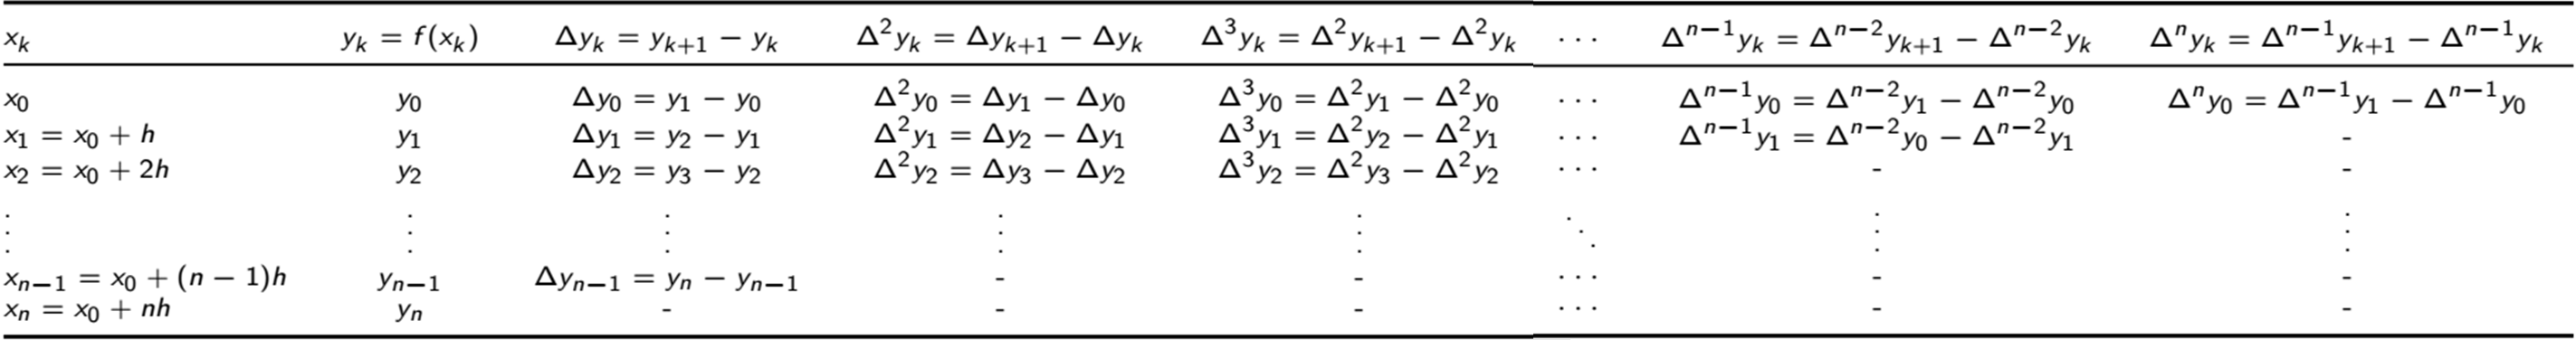
\includegraphics[width=1\linewidth]{Plots/U4/tabladif} \end{center}

\textbf{Ejemplo 1}. Sea \(y=f(x)\) una función desconocida de la cual se tienen los valores tabulados \((x_k, y_k)\) que se presentan a continuación, junto con una representación gráfica de los mismos:

\begin{longtable}[]{@{}ccc@{}}
\toprule
\(k\) & \(x_k\) & \(y_k\)\tabularnewline
\midrule
\endhead
0 & 2 & 0,3010\tabularnewline
1 & 3 & 0,4771\tabularnewline
2 & 4 & 0,6021\tabularnewline
3 & 5 & 0,6990\tabularnewline
4 & 6 & 0,7781\tabularnewline
5 & 7 & 0,8451\tabularnewline
\bottomrule
\end{longtable}

\begin{center}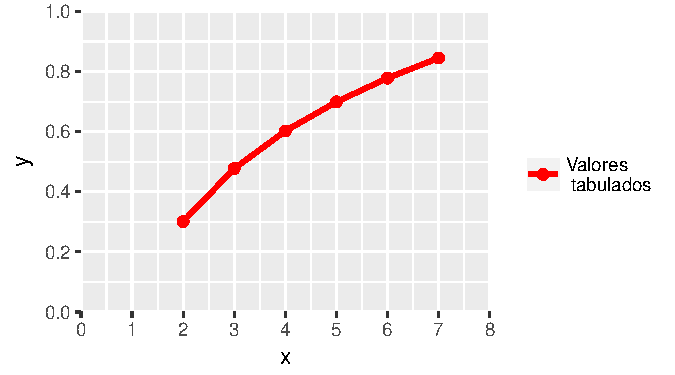
\includegraphics[width=1\linewidth]{Plots/U4/Unidad4_g1} \end{center}

La correspondiente tabla de diferencias finitas es:

\begin{longtable}[]{@{}cccccccc@{}}
\toprule
\(k\) & \(x_k\) & \(y_k\) & \(\Delta y_k\) & \(\Delta^2 y_k\) & \(\Delta^3 y_k\) & \(\Delta^4 y_k\) & \(\Delta^5 y_k\)\tabularnewline
\midrule
\endhead
0 & 2 & 0,3010 & 0,1761 & -0,0511 & 0,0230 & -0,0127 & 0,0081\tabularnewline
1 & 3 & 0,4771 & 0,1250 & -0,0281 & 0,0103 & -0,0046 & -\tabularnewline
2 & 4 & 0,6021 & 0,0969 & -0,0178 & 0,0057 & - & -\tabularnewline
3 & 5 & 0,6990 & 0,0791 & -0,0121 & - & - & -\tabularnewline
4 & 6 & 0,7781 & 0,0670 & - & - & - & -\tabularnewline
5 & 7 & 0,8451 & - & - & - & - & -\tabularnewline
\bottomrule
\end{longtable}

\textbf{Observaciones:}

\begin{itemize}
\tightlist
\item
  Si tenemos \(n+1\) puntos podemos calcular \(n\) columnas de diferencias hacia adelante.
\item
  Si la función \(f(x)\) que dio lugar a la tabla es un polinomio de orden \(q\), entonces la columna para la diferencia de orden \(q\) es constante y las siguientes columnas son todas nulas.
\item
  Por lo tanto, si en el proceso de obtención de las diferencias sucesivas de una función, las diferencias de orden \(q\) se vuelven constantes (o aproximadamente constantes), sabemos que los datos provienen exactamente (o muy aproximadamente) de un polinomio de orden \(q\).
\item
  Errores de redondeo podrían hacer que a pesar de que los datos provengan de un polinomio, no encontremos diferencias constantes.
\end{itemize}

\hypertarget{interpolaciuxf3n-de-newton-para-incrementos-constantes}{%
\section{Interpolación de Newton para incrementos constantes}\label{interpolaciuxf3n-de-newton-para-incrementos-constantes}}

\begin{itemize}
\item
  Ahora intentaremos resolver el problema de aproximar la función \(f(x)\) para valores de \(x\) que no forman parte de la tabla.
\item
  Operando con los valores de la tabla de diferencias, se comprueba que los valores tabulados \(y_k\) se pueden escribir como:

  \[
    \begin{aligned}
    y_k & = \sum_{j=0}^k \binom{k}{j} \Delta^{j} y_0 \\
        & = y_0 + k \Delta y_0 + \frac{k(k-1)}{2!}\Delta^2 y_0 + \frac{k(k-1)(k-2)}{3!}\Delta^3 y_0 + \cdots + \Delta^k y_0 
    \end{aligned}
    \]

  donde \(\Delta^{0} y_0 = y_0\).
\item
  Por ejemplo:

  \[
    y_2 = 0.3010 + 2 \cdot 0.1761 + \frac{2\cdot 1}{2!} (-0.0511) = 0.6021
    \]
\item
  Esta fórmula se emplea para proporcionar valores aproximados de \(y = f(x)\) para cualquier \(x\):

  \[
    y = f(x) \cong \sum_{j = 0}^{g} \binom{k}{j} \Delta^{j} y_0 = 
    \]
  \[
    y_0 + k \Delta y_0 + \frac{k(k-1)}{2!}\Delta^2 y_0 + \frac{k(k-1)(k-2)}{3!}\Delta^3 y_0 + \cdots
    \]

  donde \(g\) es el orden de la aproximación, \(\Delta^{0} y_0 = y_0\) y \(k = \frac{x-x_0}{h}\).
\item
  Si \(x_0 < x < x_n\), este proceso se llama \textbf{interpolación} y la fórmula anterior, \textbf{Fórmula de interpolación de Newton para incrementos constantes}.
\item
  Si para hallar una aproximación sólo empleamos la diferencia de 1º orden, tenemos una \textbf{interpolación lineal}: \(f(x) \approx y_0 + k \Delta y_0\). El polinomio interpolador es de grado 1: una recta que pasa por los puntos \((x_0, y_0)\) y \((x_1, y_1)\).
\item
  Si empleamos hasta la diferencia de 2º orden, tenemos una \textbf{interpolación cuadrática}: \(f(x) \approx y_0 + k \Delta y_0 + \frac{k(k-1)}{2!}\Delta^2 y_0\). El polinomio interpolador es de grado 2: una parábola que pasa por los puntos \((x_0, y_0)\), \((x_1, y_1)\) y \((x_2, y_2)\).
\item
  Cuantas más diferencias empleemos, el polinomio interpolador es de mayor orden y puede brindar mejores aproximaciones.
\item
  Si empleamos las \(n\) diferencias, el polinomio interpolador es el único polinomio de grado \(n\) que pasa exactamente por los \(n + 1\) puntos tabulados.
\end{itemize}

\textbf{Retomando el Ejemplo 1}: vamos a aproximar el valor de \(f(2,3)\). Recordamos la tabla de diferencias y el gráfico:

\begin{longtable}[]{@{}lllllll@{}}
\toprule
\(x_k\) & \(y_k\) & \(\Delta y_k\) & \(\Delta^2 y_k\) & \(\Delta^3 y_k\) & \(\Delta^4 y_k\) & \(\Delta^5 y_k\)\tabularnewline
\midrule
\endhead
2 & 0,3010 & 0,1761 & -0,0511 & 0,0230 & -0,0127 & 0,0081\tabularnewline
3 & 0,4771 & 0,1250 & -0,0281 & 0,0103 & -0,0046 & -\tabularnewline
4 & 0,6021 & 0,0969 & -0,0178 & 0,0057 & - & -\tabularnewline
5 & 0,6990 & 0,0791 & -0,0121 & - & - & -\tabularnewline
6 & 0,7781 & 0,0670 & - & - & - & -\tabularnewline
7 & 0,8451 & - & - & - & - & -\tabularnewline
\bottomrule
\end{longtable}

\begin{center}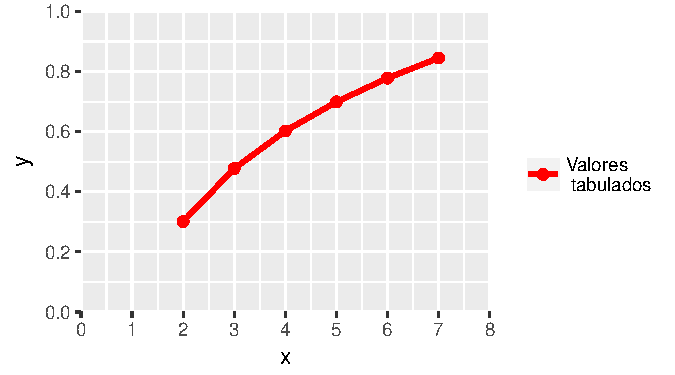
\includegraphics[width=1\linewidth]{Plots/U4/Unidad4_g1} \end{center}

\begin{itemize}
\item
  ¿Hasta qué orden de diferencias deberíamos incluir? Es decir, ¿qué grado elegimos para el polinomio interpolador?
\item
  Viendo el gráfico podemos pensar que una función cuadrática puede proveer un buen ajuste.
\item
  Por eso, proponemos un polinomio interpolador de grado 2, usando hasta la diferencia de segundo orden:

  \begin{itemize}
  \tightlist
  \item
    \(x = 2,3\)
  \item
    \(x_0 = 2\)
  \item
    \(h = 1\)
  \item
    \(k = \frac{x-x_0}{h} = \frac{2,3-2}{1} = 0,3\)
  \item
    \(y_0 = 0,3010\); \(\Delta y_0 = 0,1761\); \(\Delta^2 y_0 = -0,0511\)
  \end{itemize}
\end{itemize}

\[
\begin{aligned}
y = f(2,3) &\approx y_0 + k \Delta y_0 + \frac{k(k-1)}{2!}\Delta^2 y_0 \\
    & = 0,3010 + k \cdot 0,1761 + \frac{k(k-1)}{2!} \cdot (-0,0511) \\
  & = 0,3010 + 0,3 \cdot 0,1761 + \frac{0,3 (0,3-1)}{2} (-0,0511) \\
  & = 0,3592
\end{aligned}
\]

\begin{itemize}
\tightlist
\item
  ¿Podemos encontrar la expresión del polinomio interpolador que acabamos de usar?
\item
  Sí, sólo debemos reemplazar \(k\) en la fórmula anterior por \(k = \frac{x-x_0}{h} = \frac{x-2}{1} = x-2\):
\end{itemize}

\[
\begin{aligned}
y = f(x) &\approx 0,3010 + k \cdot 0,1761 + \frac{k(k-1)}{2!} \cdot (-0,0511) \\
    & = 0,3010 + (x-2) \cdot 0,1761 + \frac{(x-2)(x-2-1)}{2!} \cdot (-0,0511) \\
  & = -0,02555 x^2 + 0,30385 x - 0,2045
\end{aligned}
\]

\begin{itemize}
\tightlist
\item
  Al representar gráficamente el polinomio interpolador, observamos que ajusta exactamente a los 3 primeros puntos tabulados y parece dar una aproximación razonable para \(x = 2,3\).
\end{itemize}

\begin{center}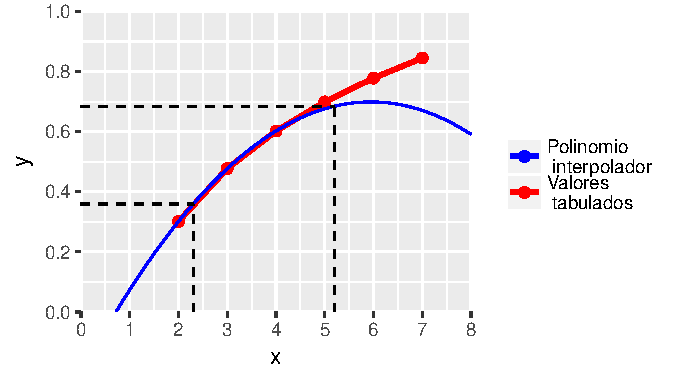
\includegraphics[width=0.7\linewidth]{Plots/U4/Unidad4_g2} \end{center}

\begin{itemize}
\item
  Sin embargo, si queremos interpolar para \(x = 5,2\), este polinomio no parece ser muy útil, porque \(5,2\) se aleja demasiado de los puntos ajustados.
\item
  Por eso, siempre ``corremos'' el valor inicial \(x_0\) hasta el inmediato inferior del que queremos aproximar.
\item
  Entonces, para \(x=5,2\) tomamos:

  \begin{itemize}
  \tightlist
  \item
    \(x_0 = 5\)
  \item
    \(h = 1\)
  \item
    \(k = \frac{x-x_0}{h} = \frac{5,2-5}{1} = 0,2\)
  \item
    \(y_0 = 0,6990\); \(\Delta y_0 = 0,0791\); \(\Delta^2 y_0 = -0,0121\)
  \end{itemize}
\end{itemize}

\[
\begin{aligned}
y = f(5,2) &\approx y_0 + k \Delta y_0 + \frac{k(k-1)}{2!}\Delta^2 y_0 \\
  & = 0,6990 + 0,2 \cdot 0,0791 + \frac{0,2 (0,2-1)}{2} (-0,0121) \\
  & = 0,7158
\end{aligned}
\]

\begin{itemize}
\tightlist
\item
  Así, con \(x_0 = 5\), la expresión del polinomio interpolador queda \(f(x) \approx -0,00605 x^2 + 0,14565 x - 0,122\) y ajusta exactamente a los tres últimos puntos tabulados:
\end{itemize}

\begin{center}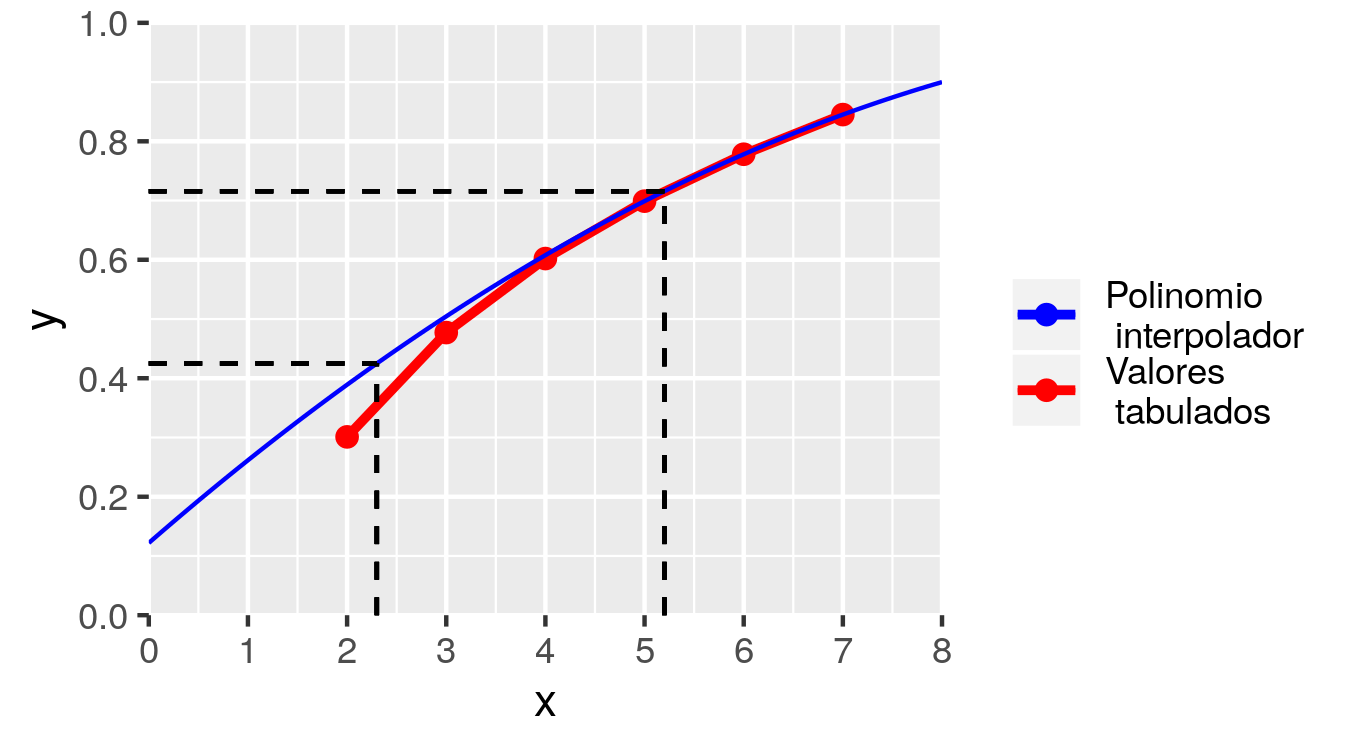
\includegraphics[width=0.95\linewidth]{Plots/U4/Unidad4_g3} \end{center}

\begin{itemize}
\tightlist
\item
  Retomemos la interpolación cuadrática para \(x=2,3\) que nos dio \(f(x) \approx 0,3592\).
\item
  ¿Cómo cambiará la aproximación si usamos polinomios de mayor orden, incluyendo diferencias superiores?
\item
  Incrementar un grado en el orden del polinomio interpolador es muy sencillo, porque solamente tenemos que sumarle un término al polinomio de grado inferior.
\item
  En el ejemplo con \(x = 2.3\); \(x_0=2\); \(h = 1\); \(k = 0.3\):
\end{itemize}

\begin{longtable}[]{@{}cc@{}}
\toprule
Grado & \(f(2.3) \approx\)\tabularnewline
\midrule
\endhead
1 & \(y_0 + k \Delta y_0 = 0.3538\)\tabularnewline
2 & \(0.3538 + \frac{k(k-1)}{2!}\Delta^2 y_0 = 0.3592\)\tabularnewline
3 & \(0.3592 + \frac{k(k-1)(k-2)}{3!}\Delta^3 y_0 = 0.3606\)\tabularnewline
4 & \(0.3606 + \frac{k(k-1)(k-2)(k-3)}{4!}\Delta^4 y_0 = 0.3611\)\tabularnewline
5 & \(0.3611 + \frac{k(k-1)(k-2)(k-3)(k-4)}{5!}\Delta^5 y_0 = 0.3613\)\tabularnewline
\bottomrule
\end{longtable}

\begin{itemize}
\tightlist
\item
  La función que generó la tabla de este ejemplo es el logaritmo en base 10, es decir, que el valor exacto es \(f(2,3) = log(2,3) = 0,3617\).
\item
  Con esta información, podemos calcular el Error Relativo que resulta de hacer las aproximaciones anteriores:
\end{itemize}

\begin{longtable}[]{@{}ccc@{}}
\toprule
Grado & \(f(2.3) \approx\) & ER\tabularnewline
\midrule
\endhead
1 & \(0.3538\) & 0.0218\tabularnewline
2 & \(0.3592\) & 0.0070\tabularnewline
3 & \(0.3606\) & 0.0032\tabularnewline
4 & \(0.3611\) & 0.0018\tabularnewline
5 & \(0.3613\) & 0.0012\tabularnewline
\bottomrule
\end{longtable}

Polinomios interpoladores con \(x_0=2\):

\begin{center}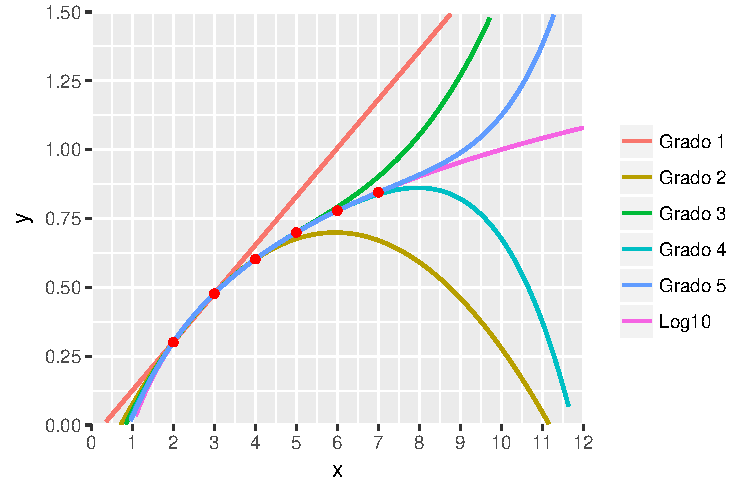
\includegraphics[width=0.9\linewidth]{Plots/U4/Unidad4_g4} \end{center}

\begin{itemize}
\tightlist
\item
  Ahora vamos a realizar una interpolación cúbica para \(x=6.4\).
\item
  Si tomamos \(x_0 = 6\), nos faltan las diferencias de 2° y 3° orden y no podemos obtener el polinomio deseado.
\item
  \textbf{Modificación}: tomar como \(x_0\) al inmediato superior y emplear las diferencias que se encuentran en la diagonal ascendente que comienza en dicho punto.
\item
  Se debe redefinir \(k\) y alternar signos positivos y negativos en la fórmula:
\end{itemize}

\begin{longtable}[]{@{}lllllll@{}}
\toprule
\(x_k\) & \(y_k\) & \(\Delta y_k\) & \(\Delta^2 y_k\) & \(\Delta^3 y_k\) & \(\Delta^4 y_k\) & \(\Delta^5 y_k\)\tabularnewline
\midrule
\endhead
2 & 0,3010 & 0,1761 & -0,0511 & 0,0230 & -0,0127 & 0,0081\tabularnewline
3 & 0,4771 & 0,1250 & -0,0281 & 0,0103 & -0,0046 & -\tabularnewline
4 & 0,6021 & 0,0969 & -0,0178 & 0,0057 & - & -\tabularnewline
5 & 0,6990 & 0,0791 & -0,0121 & - & - & -\tabularnewline
6 & 0,7781 & 0,0670 & - & - & - & -\tabularnewline
7 & 0,8451 & - & - & - & - & -\tabularnewline
\bottomrule
\end{longtable}

\(x_0 = 7\)

\(k = \frac{x_0-x}{h} = \frac{7-6.4}{1} = 0.6\)

\(y_0 = 0,8451\); \(\Delta y_0 = 0,0670\); \(\Delta^2 y_0 = -0.0121\); \(\Delta^3 y_0 = 0.0057\)

\[
\begin{aligned}
y = f(6.4) &\approx y_0 - k \Delta y_0 + \frac{k(k-1)}{2!}\Delta^2 y_0 - \frac{k(k-1)(k-2)}{3!}\Delta^3 y_0  \\
  & = 0.8451 - 0,6 \cdot 0.0670 + \frac{0.6 (0.6-1)}{2} (-0.0121) - \frac{0.6(0.6-1)(0.6-2)}{6} 0.0057\\
  & = 0.8063
\end{aligned}
\]

\textbf{Ejemplo 2}. Dada la siguiente función tabulada, interpolar para \(x = 3.2\).

\begin{longtable}[]{@{}cc@{}}
\toprule
\(x\) & \(y=f(x)\)\tabularnewline
\midrule
\endhead
0 & 2\tabularnewline
2 & 8\tabularnewline
4 & 62\tabularnewline
6 & 212\tabularnewline
8 & 506\tabularnewline
10 & 992\tabularnewline
\bottomrule
\end{longtable}

La tabla de diferencias es:

\begin{longtable}[]{@{}cccccc@{}}
\toprule
\(x_k\) & \(y_k=f(x_k)\) & \(\Delta y_k\) & \(\Delta^2 y_k\) & \(\Delta^3 y_k\) & \(\Delta^4 y_k\)\tabularnewline
\midrule
\endhead
0 & 2 & 6 & 48 & 48 & 0\tabularnewline
2 & 8 & 54 & 96 & 48 & 0\tabularnewline
4 & 62 & 150 & 144 & 48 & -\tabularnewline
6 & 212 & 294 & 192 & - & -\tabularnewline
8 & 506 & 486 & - & - & -\tabularnewline
10 & 992 & - & - & - & -\tabularnewline
\bottomrule
\end{longtable}

\begin{itemize}
\tightlist
\item
  Las diferencias de orden 3 son constantes. Esto significa que la función \(f(x)\) es exactamente un polinomio de grado 3.
\item
  Es decir, si usamos hasta la diferencia de orden 3, con la fórmula de Newton podemos hallar exactamente el valor de \(f(x)\) para cualquier \(x\) (y no importa cuál valor tomamos como \(x_0\)).
\end{itemize}

Continuando con el objetivo de hallar \(f(3.2)\):

\begin{itemize}
\tightlist
\item
  \(x = 3.2\)
\item
  \(x_0 = 2\)
\item
  \(h = 2\)
\item
  \(k = \frac{x-x_0}{h} = \frac{3.2-2}{2} = 0.6\)
\item
  \(y_0 = 8\); \(\Delta y_0 = 54\); \(\Delta^2 y_0 = 96\); \(\Delta^3 y_0 = 48\)
\end{itemize}

\[
\begin{aligned}
y = f(3.2) &= y_0 + k \Delta y_0 + \frac{k(k-1)}{2!}\Delta^2 y_0 + \frac{k(k-1)(k-2)}{3!}\Delta^3 y_0\\
  & = 8 + 0.6 \cdot 54 + \frac{0.6 (0.6-1)}{2} 96 + \frac{0.6 (0.6-1)(0.6-2)}{6} 48 \\
  & = 31.568
\end{aligned}
\]

\begin{itemize}
\tightlist
\item
  Ahora vamos a interpolar para \(x = 9\).
\item
  Si tomamos como \(x_0\) al inmediato inferior, es decir, \(x_0 = 8\), nos faltan dos diferencias para completar el cálculo.
\item
  Pero como tenemos diferencias constantes y la verdadera función es un polinomio, cualquier punto de partida nos dará el valor exacto de \(f(9)\).
\item
  Así que podemos tomar, por ejemplo, el primer renglón de la tabla: \(x_0=0\):
\item
  \(x = 9\)
\item
  \(x_0 = 0\)
\item
  \(h = 2\)
\item
  \(k = \frac{x-x_0}{h} = \frac{9-0}{2} = 4.5\)
\item
  \(y_0 = 2\); \(\Delta y_0 = 6\); \(\Delta^2 y_0 = 48\); \(\Delta^3 y_0 = 48\)
\end{itemize}

\[
\begin{aligned}
y = f(9) &= y_0 + k \Delta y_0 + \frac{k(k-1)}{2!}\Delta^2 y_0 + \frac{k(k-1)(k-2)}{3!}\Delta^3 y_0\\
  & = 2 + 4.5 \cdot 6 + \frac{4.5 (4.5-1)}{2} 48 + \frac{4.5 (4.5-1)(4.5-2)}{6} 48 \\
  & = 722
\end{aligned}
\]

\begin{itemize}
\tightlist
\item
  En los ejemplos anteriores obtuvimos el valor de \(y\) para \(x\) comprendida entre dos valores \(x_k\) de la tabla (\emph{interpolación}).
\item
  Ahora vamos a calcular el valor de \(y\) para una \(x\) fuera del rango de los valores de \(x_k\) en la tabla.
\item
  Esto se llama \textbf{extrapolación}.
\end{itemize}

\textbf{Ejemplo 3}. Extrapolar para \(x = -1\).

\begin{itemize}
\tightlist
\item
  \(x = -1\)
\item
  \(x_0 = 0\)
\item
  \(h = 2\)
\item
  \(k = \frac{x-x_0}{h} = \frac{-1-0}{2} = -0.5\)
\item
  \(y_0 = 2\); \(\Delta y_0 = 6\); \(\Delta^2 y_0 = 48\); \(\Delta^3 y_0 = 48\)
\end{itemize}

\[
\begin{aligned}
y = f(-1) &= y_0 + k \Delta y_0 + \frac{k(k-1)}{2!}\Delta^2 y_0 + \frac{k(k-1)(k-2)}{3!}\Delta^3 y_0\\
  & = 2 - 0.5 \cdot 6 + \frac{- 0.5 (- 0.5-1)}{2} 48 + \frac{- 0.5 (- 0.5-1)(- 0.5-2)}{6} 48 \\
  & = 2
\end{aligned}
\]

\textbf{Ejemplo 4}. Extrapolar para \(x = 11\).

\begin{itemize}
\tightlist
\item
  \(x = 11\)
\item
  \(x_0 = 0\)
\item
  \(h = 2\)
\item
  \(k = \frac{x-x_0}{h} = \frac{11-0}{2} = 5.5\)
\item
  \(y_0 = 2\); \(\Delta y_0 = 6\); \(\Delta^2 y_0 = 48\); \(\Delta^3 y_0 = 48\)
\end{itemize}

\[
y = f(11) = \cdots = 1322
\]

\hypertarget{interpolaciuxf3n-de-lagrange}{%
\section{Interpolación de Lagrange}\label{interpolaciuxf3n-de-lagrange}}

\begin{itemize}
\tightlist
\item
  Como ya mencionamos, en la interpolación lineal se utiliza un segmento rectilíneo que pasa por dos puntos que se conocen.
\item
  De nuestros conocimientos de Geometría sabemos que la ecuación de la recta que pasa por dos puntos \((x_0, y_0)\) y \((x_1, y_1)\) es:
\end{itemize}

\[
y = f(x) = y_0 + \frac{y_1 - y_0}{x_1 - x_0} (x - x_0)
\]

\begin{itemize}
\item
  Es fácil ver que la recta anterior pasa por los puntos dados, ya que \(f(x_0) = y_0\) y \(f(x_1) = y_1\).
\item
  Lagrange propuso reescribir la recta anterior como:
\end{itemize}

\[
f(x) = \frac{x - x_1}{x_0 - x_1} y_0 + \frac{x - x_0}{x_1 - x_0} y_1
\]

\begin{itemize}
\tightlist
\item
  Esta expresión se puede extender para obtener polinomios de grados superiores que pasen por más puntos.
\item
  Por ejemplo, para hallar el polinomio que pasa por los puntos \((x_0, y_0)\), \((x_1, y_1)\) y \((x_2, y_2)\):
\end{itemize}

\[
f(x) = \frac{(x - x_1)(x - x_2)}{(x_0 - x_1)(x_0 - x_2)} y_0 + \frac{(x - x_0)(x - x_2)}{(x_1 - x_0)(x_1 - x_2)} y_1 + \frac{(x - x_0)(x - x_1)}{(x_2 - x_0)(x_2 - x_1)} y_2
\]

\begin{itemize}
\item
  Se puede ver fácilmente que este polinomio pasa exactamente por los tres puntos dados.
\item
  De la misma forma, el polinomio de grado 3 que pasa por cuatro puntos \((x_0, y_0)\), \((x_1, y_1)\), \((x_2, y_2)\) y \((x_3, y_3)\) es:
\end{itemize}

\[
\hspace{-0.5cm}
\begin{split}
f(x) = &~ \frac{(x - x_1)(x - x_2)(x - x_3)}{(x_0 - x_1)(x_0 - x_2)(x_0 - x_3)} y_0 + \frac{(x - x_0)(x - x_2)(x - x_3)}{(x_1 - x_0)(x_1 - x_2)(x_1 - x_3)} y_1 \\
& + \frac{(x - x_0)(x - x_1)(x - x_3)}{(x_2 - x_0)(x_2 - x_1)(x_2 - x_3)} y_2 + \frac{(x - x_0)(x - x_1)(x - x_2)}{(x_3 - x_0)(x_3 - x_1)(x_3 - x_2)} y_3
\end{split}
\]

\begin{itemize}
\item
  Se puede ver fácilmente que este polinomio pasa exactamente por los cuatro puntos dados.
\item
  Generalizando, la fórmula de interpolación de Lagrange para construir un polinomio de grado \(n\) que pase por \(n+1\) puntos \((x_0, y_0), (x_1, y_1), \cdots, (x_n, y_n)\) es:
\end{itemize}

\[
y = f(x) = \sum_{i = 0}^n \frac{\prod\limits_{\substack{j = 0\\ j \neq i}}^n (x - x_j)}{\prod\limits_{\substack{j = 0\\ j \neq i}}^n (x_i - x_j)} y_i
\]

\textbf{Comparación con el método de Newton}

\begin{itemize}
\item
  \textbf{Ventaja}: no requiere que los valores tabulados de \(x\) estén equiespaciados. Si lo están, ambos métodos coinciden.
\item
  \textbf{Desventaja}:

  \begin{itemize}
  \tightlist
  \item
    En ocasiones es útil considerar varios polinomios interpoladores de distinto grado para luego elegir el más adecuado.
  \item
    Con el método de Newton esto es muy sencillo, ya que como vimos se pueden construir recursivamente (por ejemplo, el de grado 3 es igual al de grado 2 más un término extra).
  \item
    En cambio, con el método de Lagrange no hay relación entre la construcción de \(P_{n-1}(x)\) y la de \(P_n(x)\); cada polinomio debe construirse individualmente realizando todos los cálculos otra vez.
  \item
    Esto implica que este método sea menos eficiente al tener que recalcular todo el polinomio si varía el número de puntos.
  \end{itemize}
\end{itemize}

\textbf{Ejemplo 5}. Emplear el método de Lagrange para interpolar el valor de la función \(f\) en \(x=2.25\), con el polinomio interpolador de grado 3 que pasa por los cuatro puntos tabulados:

\begin{longtable}[]{@{}cc@{}}
\toprule
\(x_k\) & \(y_k\)\tabularnewline
\midrule
\endhead
-1 & 0,5403\tabularnewline
0 & 1,0000\tabularnewline
2 & -0,4162\tabularnewline
2.5 & -0,8011\tabularnewline
\bottomrule
\end{longtable}

\begin{center}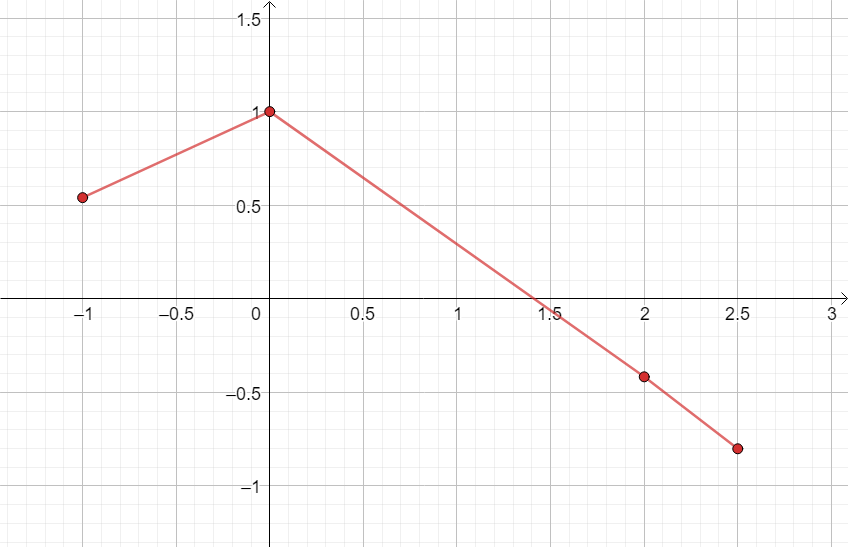
\includegraphics[width=1\linewidth]{Plots/U4/lagrej1} \end{center}

\[
\begin{split}
f(x) =& \sum_{i = 0}^3 \frac{\prod\limits_{\substack{j = 0\\ j \neq i}}^3 (x - x_j)}{\prod\limits_{\substack{j = 0\\ j \neq i}}^3 (x_i - x_j)} y_i = \\ \\
& \frac{(x - x_1)(x - x_2)(x - x_3)}{(x_0 - x_1)(x_0 - x_2)(x_0 - x_3)} y_0 + \\ \\
&\frac{(x - x_0)(x - x_2)(x - x_3)}{(x_1 - x_0)(x_1 - x_2)(x_1 - x_3)} y_1 + \\ \\
&\frac{(x - x_0)(x - x_1)(x - x_3)}{(x_2 - x_0)(x_2 - x_1)(x_2 - x_3)} y_2 + \\ \\
&\frac{(x - x_0)(x - x_1)(x - x_2)}{(x_3 - x_0)(x_3 - x_1)(x_3 - x_2)} y_3 \\ \\
\implies y = f(2.25) \approx & \frac{(2.25 - 0)(2.25 - 2)(2.25 - 2.5)}{(-1-0)(-1-2)(-1-2.5)} 0.5403 + \\ \\
&\frac{(2.25 +1)(2.25 - 2)(2.25 - 2.5)}{(0+1)(0-2)(0-2.5)} 1.0000 + \\ \\
&\frac{(2.25 +1)(2.25 - 0)(2.25 - 2.5)}{(2+1)(2-0)(2-2.5)} (-0.4162) + \\ \\
&\frac{(2.25 +1)(2.25 - 0)(2.25 - 2)}{(2.5+1)(2.5-0)(2.5-2)} (-0.8011) = \\ \\
& -0.6218 \\ \\
&\therefore f(2.25) \approx -0.6218
\end{split}
\]

Si en la fórmula anterior en lugar de reemplazar \(x\) por un valor particular (en este caso, \(2.5\)) operamos y reacomodamos los términos, podemos hallar la expresión del polinomio interpolador:

\[
f(x) = 0.1042 x^3 -0.4934 x^2 -0.1379 x+1
\]

\begin{center}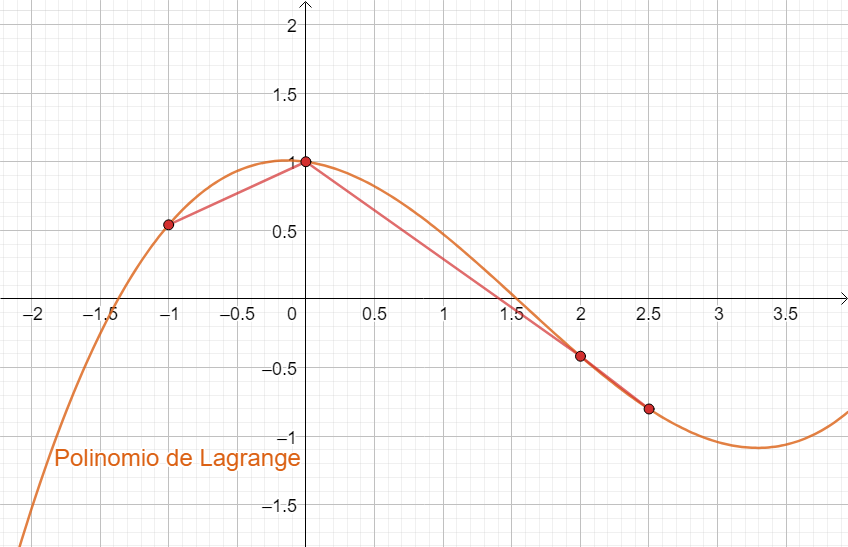
\includegraphics[width=0.6\linewidth]{Plots/U4/lagrej2} \end{center}

La función que generó los valores tabulados es \(cos(x)\):

En el rango tabulado:

\begin{center}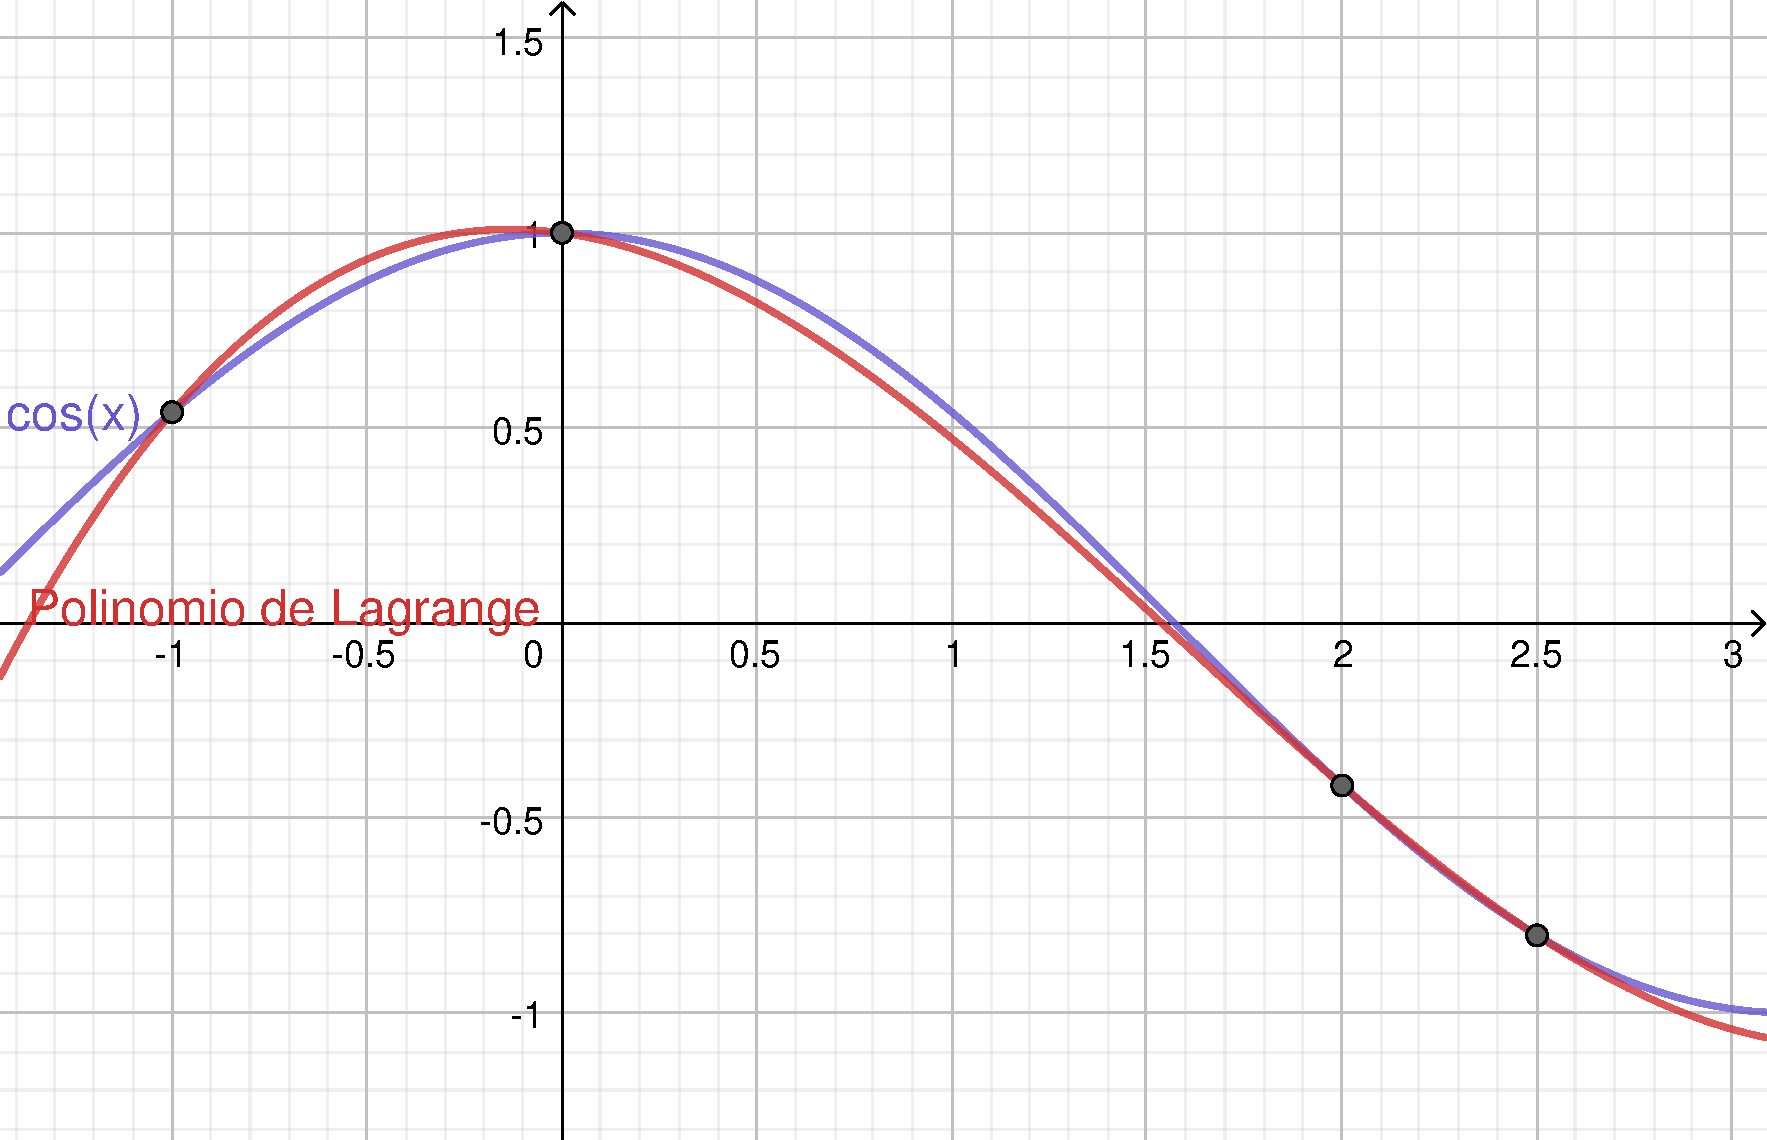
\includegraphics[width=1\linewidth]{Plots/U4/lagrange2} \end{center}

Un poco más lejos:

\begin{center}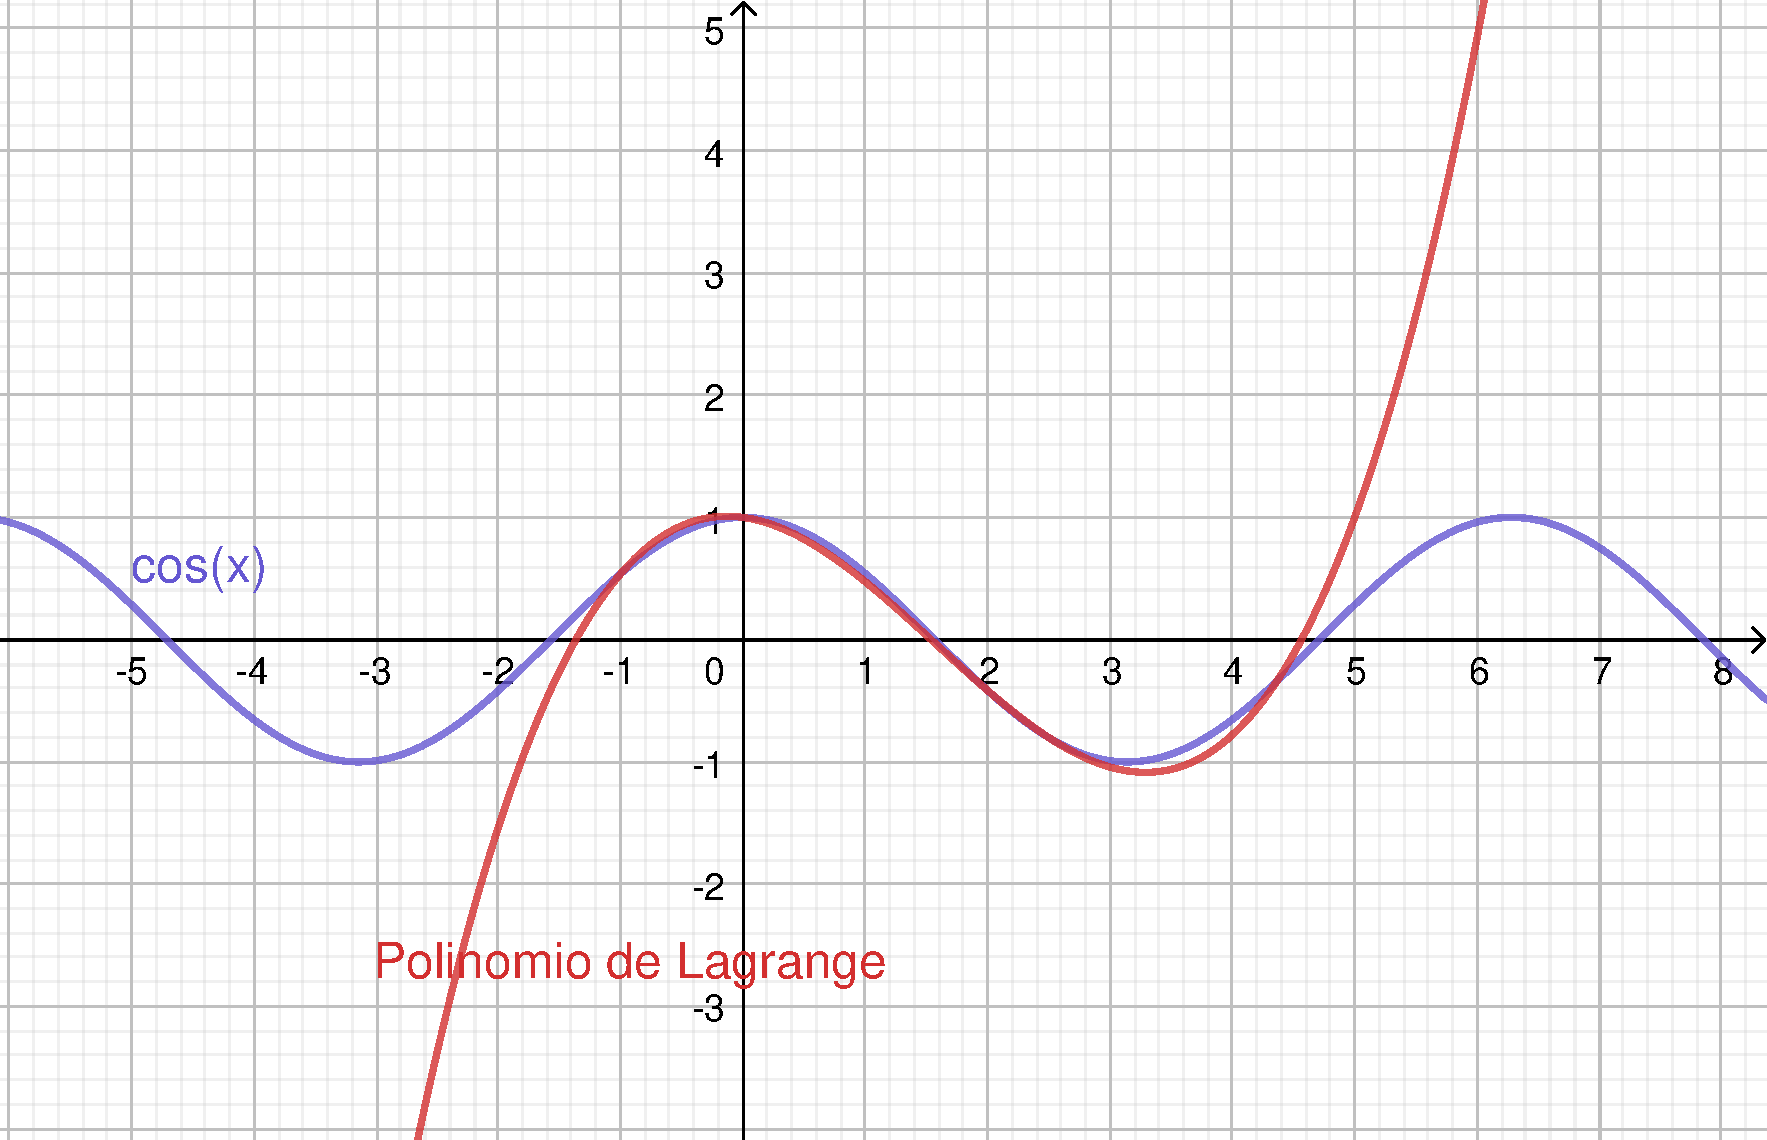
\includegraphics[width=1\linewidth]{Plots/U4/lagrange} \end{center}

Siendo \(cos(2.25) = -0.6282\), el error relativo de la aproximación fue \(|-0.6282-0.6218| / |-0.6285| = 1.02\%\)

\textbf{Interpolación inversa}

\begin{itemize}
\tightlist
\item
  El problema de interpolación consiste en determinar el valor de la función desconocida \(f(x)\) a partir de un valor conocido de \(x\).
\item
  En la \emph{interpolación inversa} se resuelve el problema contrario: determinar el valor de \(x\) conociendo el de \(f(x)\).
\item
  Podemos implementar interpolación inversa con el método de Lagrange intercambiando el rol de las columnas tabuladas \(x\) e \(y\), \textbf{pero sólo para rangos tabulados donde la función \(f\) es monótona}.
\end{itemize}

\textbf{Ejemplo 6}. Con los datos del Ejemplo 1, ¿cuál es el valor de \(x\) tal que \(f(x)=-0.75\)?

\begin{longtable}[]{@{}cc@{}}
\toprule
\(x_k\) & \(y_k\)\tabularnewline
\midrule
\endhead
-1 & 0,5403\tabularnewline
0 & 1,0000\tabularnewline
2 & -0,4162\tabularnewline
2.5 & -0,8011\tabularnewline
\bottomrule
\end{longtable}

\[\downarrow\]

\begin{longtable}[]{@{}cc@{}}
\toprule
\(x_k\) & \(y_k\)\tabularnewline
\midrule
\endhead
1,0000 & 0\tabularnewline
-0,4162 & 2\tabularnewline
-0,8011 & 2.5\tabularnewline
\bottomrule
\end{longtable}

\[
f(x) = \sum_{i = 0}^2 \frac{\prod\limits_{\substack{j = 0\\ j \neq i}}^2 (x - x_j)}{\prod\limits_{\substack{j = 0\\ j \neq i}}^2 (x_i - x_j)} y_i
\]

\[
= \frac{(x - x_1)(x - x_2)}{(x_0 - x_1)(x_0 - x_2)} y_0 + \frac{(x - x_0)(x - x_2)}{(x_1 - x_0)(x_1 - x_2)} y_1 + \frac{(x - x_0)(x - x_1)}{(x_2 - x_0)(x_2 - x_1)} y_2
\]

\[
\begin{split}
\implies f(-0.75) &\approx \frac{(-0.75+0.4162)(-0.75+0.8011)}{(1+0.4162)(1+0.8011)} 0 \\
&~ + \frac{(-0.75-1)(-0.75+0.8011)}{(-0.4162-1)(-0.4162+0.8011)} 2 \\
&~ + \frac{(-0.75-1)(-0.75+0.4162)}{(-0.8011-1)(-0.8011+0.4162)} 2.5  \\
&= 2.4347
\end{split}
\]
\(\therefore\) el valor de \(x\) tal que \(f(x)=-0.75\) es \(x \approx 2.4347\).

\textbf{Interpolación inversa}. Podemos usar la interpolación inversa para resolver ecuaciones.

\textbf{Ejemplo 7}: hallar una raiz positiva para la ecuación \(f(x)=x-4\sin(x+2) = 0\). Tabulamos algunos valores y graficamos:

\begin{longtable}[]{@{}cc@{}}
\toprule
\(x_k\) & \(y_k\)\tabularnewline
\midrule
\endhead
0 & -3.6372\tabularnewline
0.5 & -1.8939\tabularnewline
1 & 0.4355\tabularnewline
\bottomrule
\end{longtable}

\begin{center}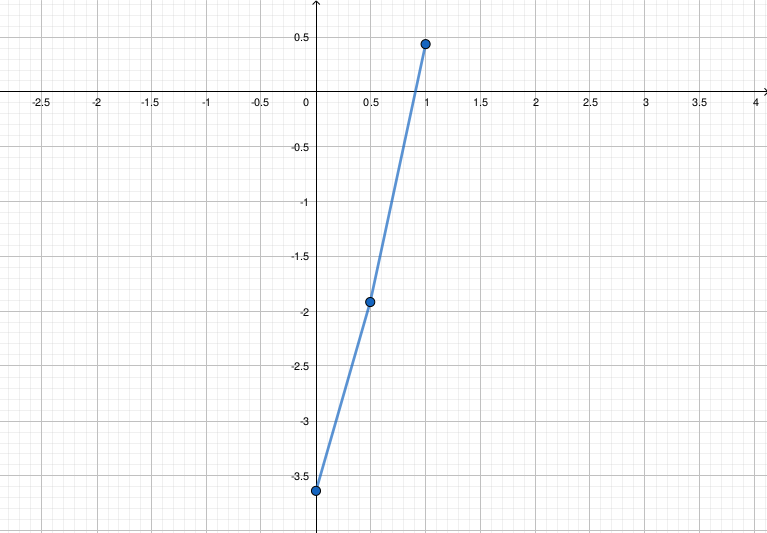
\includegraphics[width=0.75\linewidth]{Plots/U4/lagr_ecuacion1} \end{center}

Podemos usar los dos últimos puntos donde vemos que la función cortó a las abscisas y hacer una interpolación lineal, o usar los tres puntos y tener una interpolación cuadrática, o incluso agregar más puntos. Al intercambiar roles:

\begin{longtable}[]{@{}cc@{}}
\toprule
\(x_k\) & \(y_k\)\tabularnewline
\midrule
\endhead
-3.6372 & 0\tabularnewline
-1.8939 & 0.5\tabularnewline
0.4355 & 1\tabularnewline
\bottomrule
\end{longtable}

\[
\begin{split}
y = f(x) &= \frac{x - x_1}{x_0 - x_1} y_0 + \frac{x - x_0}{x_1 - x_0} y_1 \\ \\
\implies f(0) &\approx \frac{0-0.4355}{-1.8939-0.4355} 0.5 + \frac{0+1.8939}{0.4355+1.8939} 1 \\ \\
&= 0.9065 \\
\end{split}
\]

\(\therefore\) La solución positiva de la ecuación es \(x \approx 0.9065\) ya que \(f(0.9065) \approx 0\).

\hypertarget{observaciones-finales}{%
\subsection{Observaciones finales}\label{observaciones-finales}}

\begin{itemize}
\tightlist
\item
  Un polinomio de grado \(n\) ajustado a \(n+1\) puntos es único.
\item
  El polinomio de interpolación se puede expresar en varias formas distintas, pero todas son equivalentes por el punto anterior.
\item
  Si una función se aproxima mediante un polinomio de interpolación, no hay garantía de que dicho polinomio converja a la función exacta al aumentar el número de datos. En general, la interpolación mediante un polinomio de orden grande debe evitarse o utilizarse con precauciones extremas.
\item
  Aunque no existe un criterio para determinar el orden óptimo del polinomio de interpolación, generalmente se recomienda utilizar uno con orden relativamente bajo en un pequeño rango de \(x\).
\end{itemize}

\hypertarget{aproximaciuxf3n-polinomial-integraciuxf3n-y-derivaciuxf3n-numuxe9rica}{%
\chapter{Aproximación Polinomial: integración y derivación numérica}\label{aproximaciuxf3n-polinomial-integraciuxf3n-y-derivaciuxf3n-numuxe9rica}}

\hypertarget{integraciuxf3n-numuxe9rica}{%
\section{Integración numérica}\label{integraciuxf3n-numuxe9rica}}

\begin{itemize}
\tightlist
\item
  Dada la función \(y = f(x)\) definida en forma tabular con a través de \(n+1\) valores de \(x\) equiespaciados \(x_0, x_1 = x_0 + h, \cdots, x_n = x_0 + nh\), se desea hallar una aproximación de la integral definida:
\end{itemize}

\begin{equation}
\label{eq:ec1}
\int_{x_0}^{x_n} f(x)dx
\end{equation}

\begin{itemize}
\tightlist
\item
  Para esto, aproximaremos a \(f(x)\) con el polinomio de Newton:
\end{itemize}

\begin{equation}
\label{eq:ec2}
f(x) \cong y_0 + k \Delta y_0 + \frac{k(k-1)}{2!}\Delta^2 y_0 \\
+ \frac{k(k-1)(k-2)}{3!}\Delta^3 y_0 + \cdots
\end{equation}

\[
k = \frac{x-x_0}{h}
\]

\begin{itemize}
\tightlist
\item
  En \eqref{eq:ec1} la variable es \(x\), mientras que en \eqref{eq:ec2} la variable está expresada como \(k = (x - x_0)/h\), por lo tanto para poder reemplazar \eqref{eq:ec2} en \eqref{eq:ec1} se debe realizar un cambio de variables:
\end{itemize}

\[
k = \frac{x-x_0}{h} \implies
\begin{cases}
x = x_0 + hk \\
dx = hdk \\
x = x_0 \implies k = \frac{x_0-x_0}{h} = 0 \\
x = x_n \implies k = \frac{x_n-x_0}{h} = \frac{x_0 + nh -x_0}{h} =n \\
\end{cases}
\]

\begin{itemize}
\tightlist
\item
  Luego:
\end{itemize}

\[
\begin{aligned}
& \int_{x_0}^{x_n} f(x)dx \\
& \cong \int_{0}^{n} \Big( y_0 + k \Delta y_0 + \frac{k(k-1)}{2!}\Delta^2 y_0 + \frac{k(k-1)(k-2)}{3!}\Delta^3 y_0 + \cdots \Big) h\,dk \\
& = h \int_{0}^{n} \Big[ y_0 + k \Delta y_0 + \Big( \frac{k^2}{2} - \frac{k}{2} \Big) \Delta^2 y_0 + \Big( \frac{k^3}{6} - \frac{k^2}{2} + \frac{k}{3} \Big) \Delta^3 y_0  + \cdots \Big] dk \\
&= h \Big[ 
\left.
y_0 k + \frac{k^2}{2} \Delta y_0 + \Big( \frac{k^3}{6} - \frac{k^2}{4} \Big) \Delta^2 y_0 + \Big( \frac{k^4}{24} - \frac{k^3}{6} + \frac{k^2}{6} \Big) \Delta^3 y_0  + \cdots
\Big] \right\vert_{0}^{n} \\
&= h \Big[ y_0 n + \frac{n^2}{2} \Delta y_0 + \Big( \frac{n^3}{6} - \frac{n^2}{4} \Big) \Delta^2 y_0 + \Big( \frac{n^4}{24} - \frac{n^3}{6} + \frac{n^2}{6} \Big) \Delta^3 y_0  + \cdots
\Big]
\end{aligned}
\]

\textbf{Ejemplo}. Se tienen los siguientes valores tabulados de \(f(x)\) y se desea hallar su integral entre 0 y 6.

\begin{longtable}[]{@{}cc@{}}
\toprule
\(x\) & \(y=f(x)\)\tabularnewline
\midrule
\endhead
0.0 & 2.00\tabularnewline
0.5 & 3.13\tabularnewline
1.0 & 2.14\tabularnewline
1.5 & 1.14\tabularnewline
2.0 & 1.78\tabularnewline
2.5 & 2.64\tabularnewline
3.0 & 2.25\tabularnewline
3.5 & 1.53\tabularnewline
4.0 & 1.75\tabularnewline
4.5 & 2.34\tabularnewline
5.0 & 2.24\tabularnewline
5.5 & 1.77\tabularnewline
6.0 & 1.78\tabularnewline
\bottomrule
\end{longtable}

\begin{center}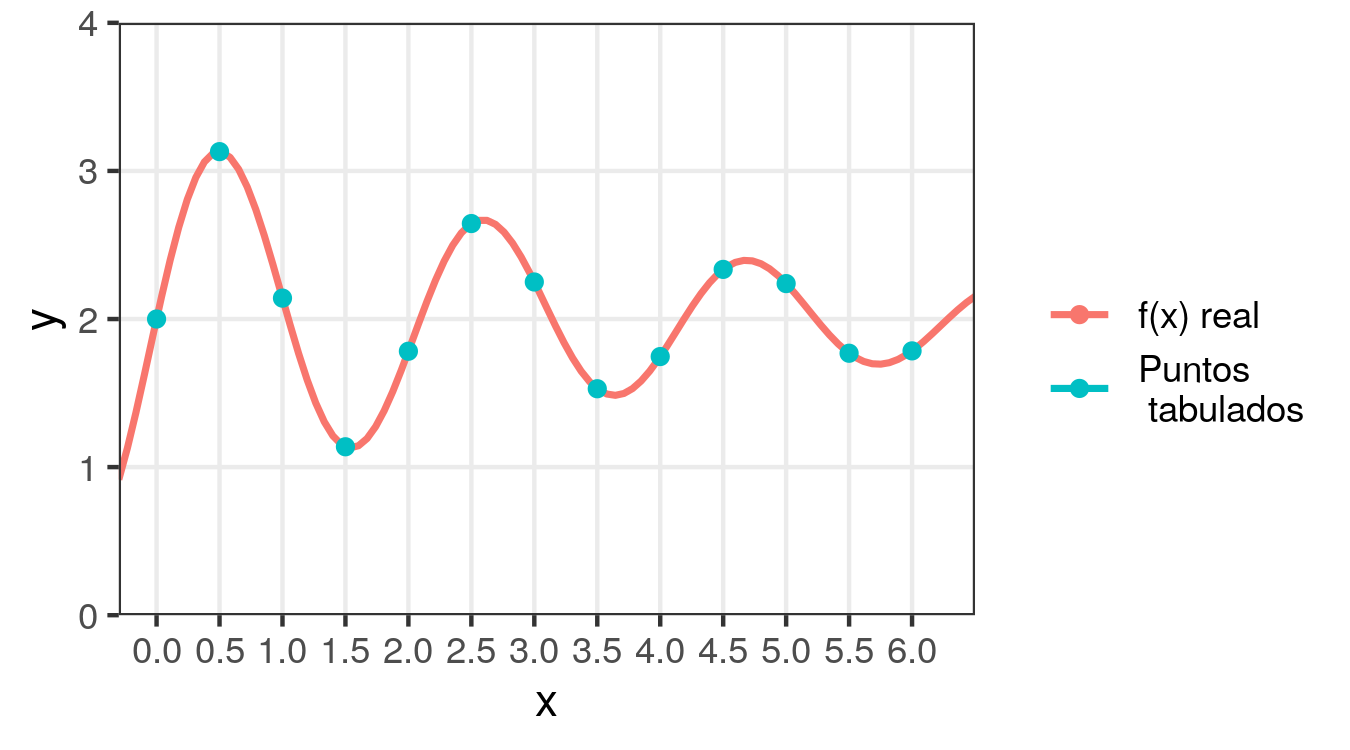
\includegraphics[width=1\linewidth]{Plots/U4/Unidad4_2_g} \end{center}

La curva roja es la verdadera función \(f(x)\) que originó la tabla, la cual suponemos desconocida o difícil de integrar.

\hypertarget{fuxf3rmula-trapecial}{%
\subsection{Fórmula trapecial}\label{fuxf3rmula-trapecial}}

\begin{itemize}
\tightlist
\item
  Si la interpolación se limita al primer orden y la integral sólo se calcula entre los dos primeros valores de \(x\), se obtiene:
\end{itemize}

\begin{gather*}
\int_{x_0}^{x_1} f(x)dx \cong  \int_{0}^{1} \Big( y_0 + k \Delta y_0 \Big) hdk = h \left. \Big( y_0 k + \frac{k^2}{2} \Delta y_0 \Big) \right\vert_{0}^{1} \\
= h \Big( y_0 + \frac{\Delta y_0}{2} \Big) = h \Big( y_0 + \frac{y_1 - y_0}{2} \Big) = \frac{h}{2} (y_0 + y_1)
\end{gather*}

\begin{itemize}
\tightlist
\item
  En el ejemplo:
\end{itemize}

\[
\int_{0}^{0.5} f(x)dx \cong  \frac{0.5}{2} (3.13 + 2) = 1.2825
\]

\begin{itemize}
\tightlist
\item
  Geométricamente, esto equivale al área \(A_1\) del trapecio formado por la recta de interpolación y el eje de las abscisas, entre \(x_0\) y \(x_1\):
\end{itemize}

\[A_2=1.2825\]

\begin{center}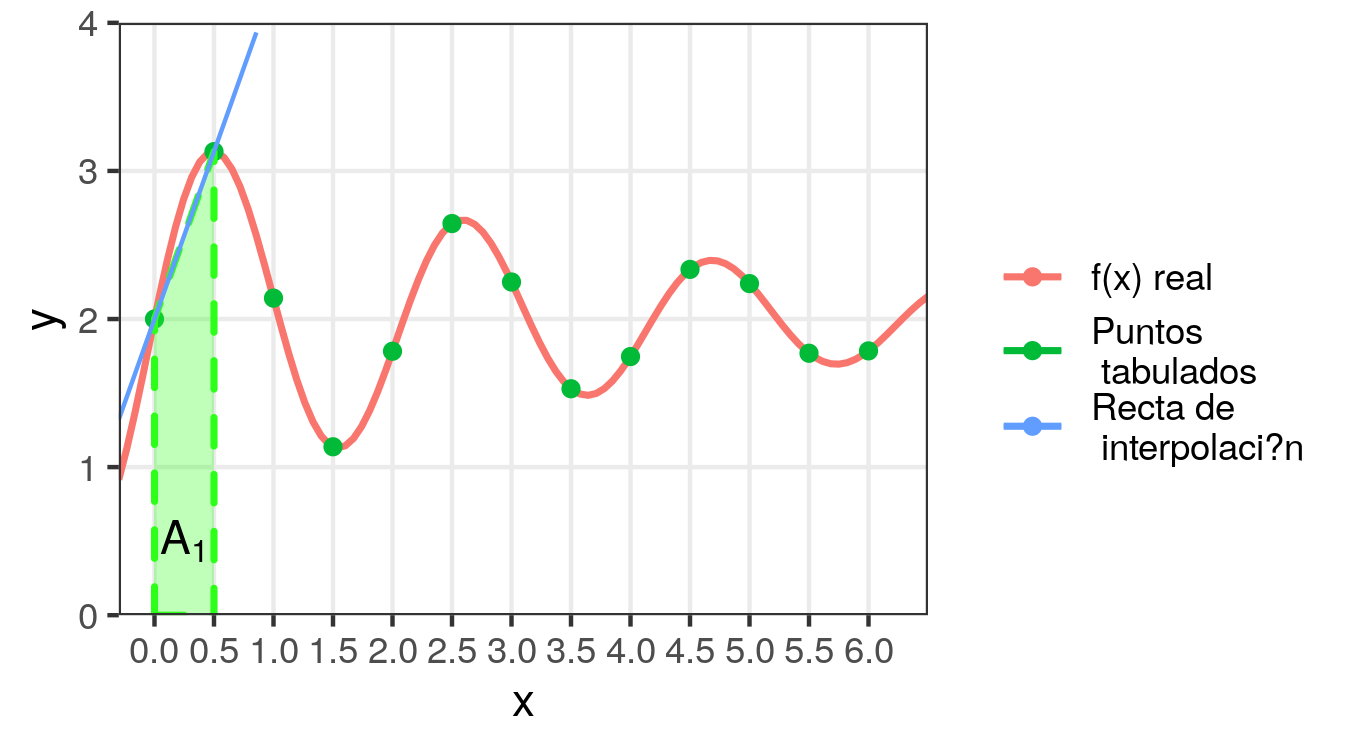
\includegraphics[width=1\linewidth]{Plots/U4/Unidad4_2_g2} \end{center}

\begin{itemize}
\tightlist
\item
  De manera semejante, se puede emplear la interpolación lineal de Newton para obtener una aproximación de la integral entre \(x_1\) y \(x_2\):
\end{itemize}

\[
\int_{x_1}^{x_2} f(x)dx \cong A_2 = \frac{h}{2} (y_1 + y_2)
\]

\[A_2=1.3175\]

\begin{center}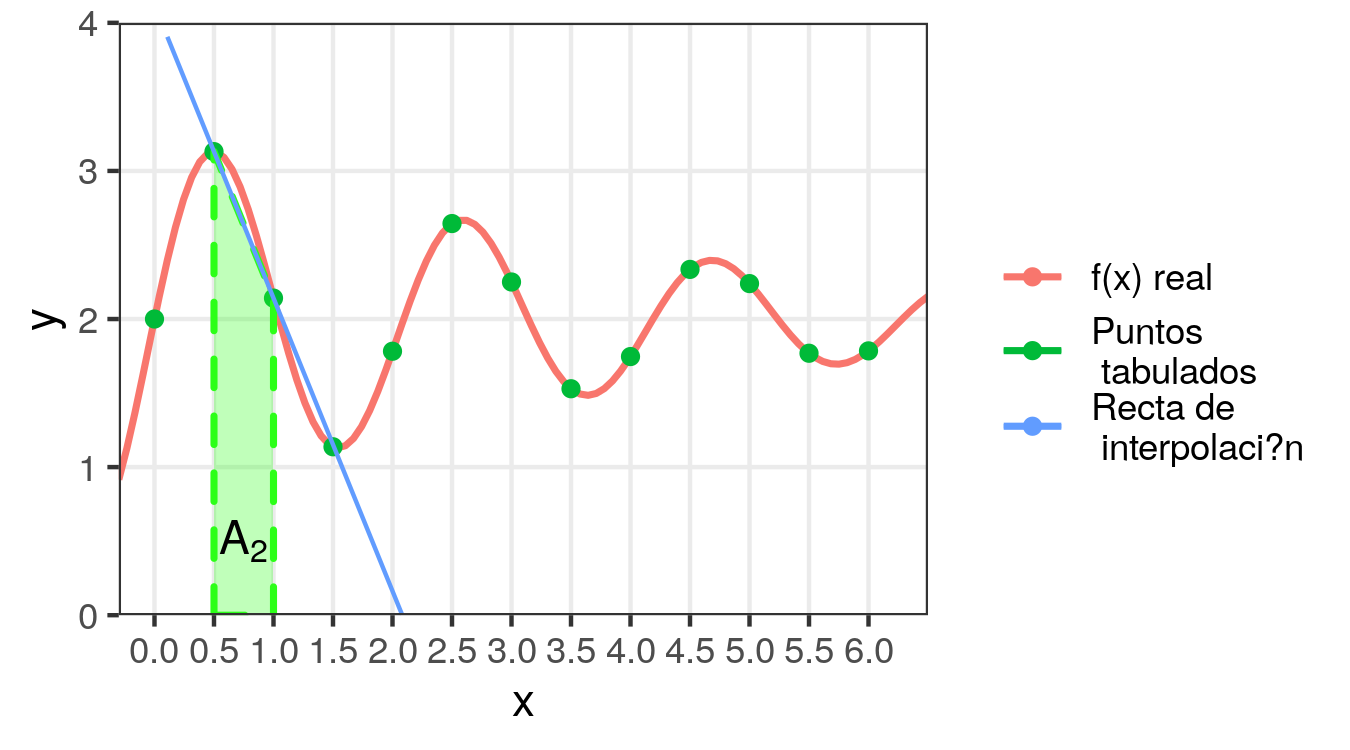
\includegraphics[width=1\linewidth]{Plots/U4/Unidad4_2_g3} \end{center}

\begin{itemize}
\tightlist
\item
  Y sucesivamente para todos los intervalos:
\end{itemize}

\[
\int_{x_{i-1}}^{x_i} f(x)dx \cong A_i = \frac{h}{2} (y_{i-1} + y_i) \quad i = 1, \cdots, n
\]

\begin{itemize}
\tightlist
\item
  De modo que la suma de las áreas de los trapecios \(A_i\) resulta ser la aproximación para la integral entre \(x_0\) y \(x_n\):
\end{itemize}

\[
\int_{x_{0}}^{x_n} f(x)dx \cong \sum_{i=1}^n A_i = \sum_{i=1}^n \frac{h}{2} (y_{i-1} + y_i) = \frac{h}{2} \Big( y_0 + y_n + 2 \sum_{i = 1}^{n-1} y_i \Big)
\]

\begin{itemize}
\tightlist
\item
  La fórmula hallada se conoce como \textbf{fórmula trapecial} y se la simboliza con:
\end{itemize}

\[
A_{1/2} = \frac{h}{2} \Big( y_0 + y_n + 2 \sum_{i = 1}^{n-1} y_i \Big)
\]

\begin{itemize}
\tightlist
\item
  Cuanto menor sea el ancho de los intervalos \(h\) y más se acerque \(f(x)\) a una recta dentro de dichos intervalos, mejor será la aproximación así obtenida.
\item
  Gráficamente:
\end{itemize}

\begin{center}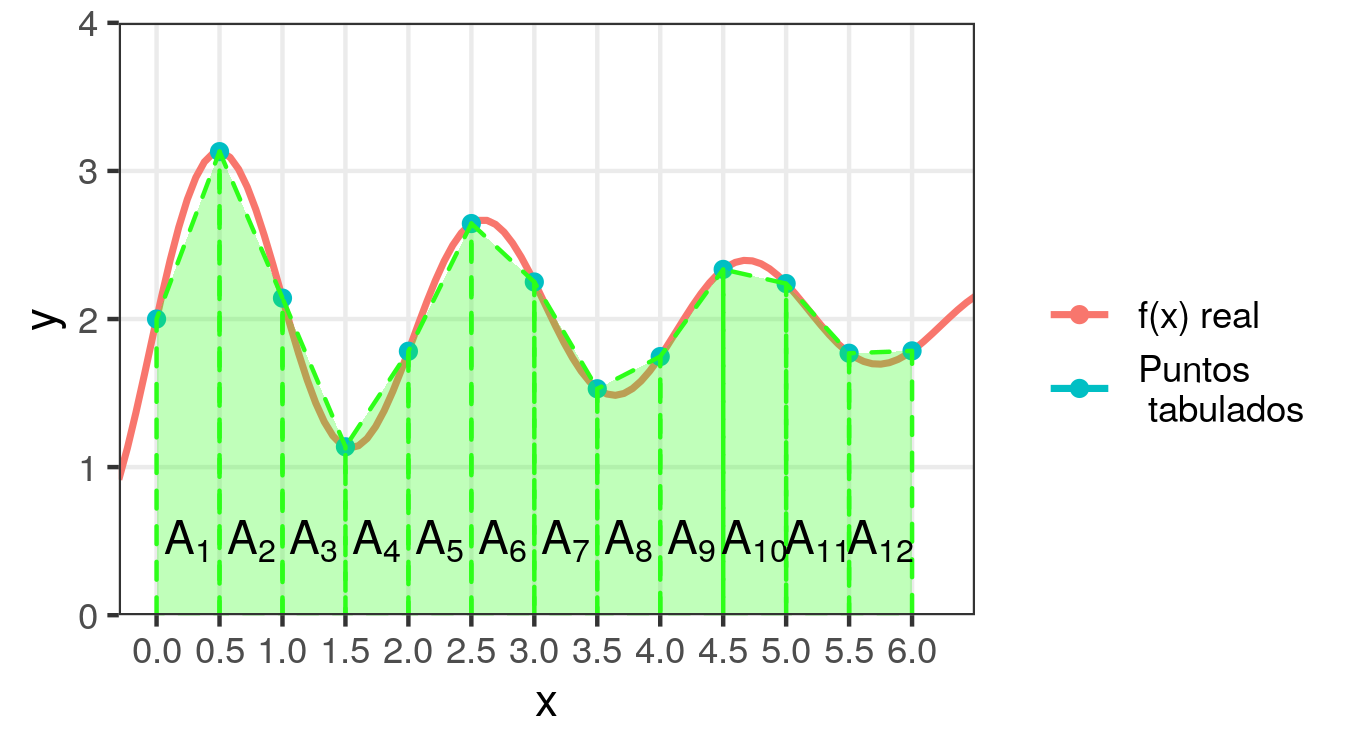
\includegraphics[width=0.85\linewidth]{Plots/U4/Unidad4_2_g4} \end{center}

\begin{itemize}
\tightlist
\item
  En el ejemplo: \(A_{1/2} = 12.3000\).
\item
  El valor exacto es: \(\int_0^{6}f(x)dx = 12.2935\), con lo cual el error relativo de la aproximación con la fórmula trapecial fue: \(0.05\%\).
\end{itemize}

\hypertarget{fuxf3rmula-de-simpson-de-13}{%
\subsection{Fórmula de Simpson de 1/3}\label{fuxf3rmula-de-simpson-de-13}}

\begin{itemize}
\tightlist
\item
  Si la interpolación es de segundo orden y la integral sólo se calcula entre los tres primeros valores de \(x\), se obtiene:
\end{itemize}

\[
\begin{aligned}
\int_{x_0}^{x_2} f(x)dx &\cong  \int_{0}^{2} \Big[ y_0 + k \Delta y_0 + \Big( \frac{k^2}{2} - \frac{k}{2} \Big) \Delta^2 y_0 \Big]  hdk \\
&= h \left. \Big[ y_0 k + \frac{k^2}{2} \Delta y_0  + \Big( \frac{k^3}{6} - \frac{k^2}{4} \Big) \Delta^2 y_0 \Big] \right\vert_{0}^{2} \\
&= h \Big[ 2y_0 + 2 \Delta y_0  + \frac{1}{3} \Delta^2 y_0 \Big]
\end{aligned}
\]

\begin{itemize}
\tightlist
\item
  Dado que \(\Delta y_0 = y_1 - y_0\) y \(\Delta^2 y_0 = \Delta y_1 - \Delta y_0 = y_2 - 2y_1 + y_0\), nos queda:
\end{itemize}

\[
\begin{aligned}
\int_{x_0}^{x_2} f(x)dx &\cong h \Big[ 2y_0 + 2 (y_1 - y_0)  + \frac{1}{3} (y_2 - 2y_1 + y_0) \Big] \\
&= \frac{h}{3} (y_0 + 4y_1 + y_2)
\end{aligned}
\]

\begin{itemize}
\tightlist
\item
  Geométricamente, esto equivale al área \(A_1\) encerrada entre el eje de las abscisas, \(x_0\) y \(x_2\) y el polinomio integrador que pasa por \((x_0, y_0)\), \((x_1, y_1)\) y \((x_2, y_2)\): \hspace{3cm} \(A_1=2.7766\)
\end{itemize}

\begin{center}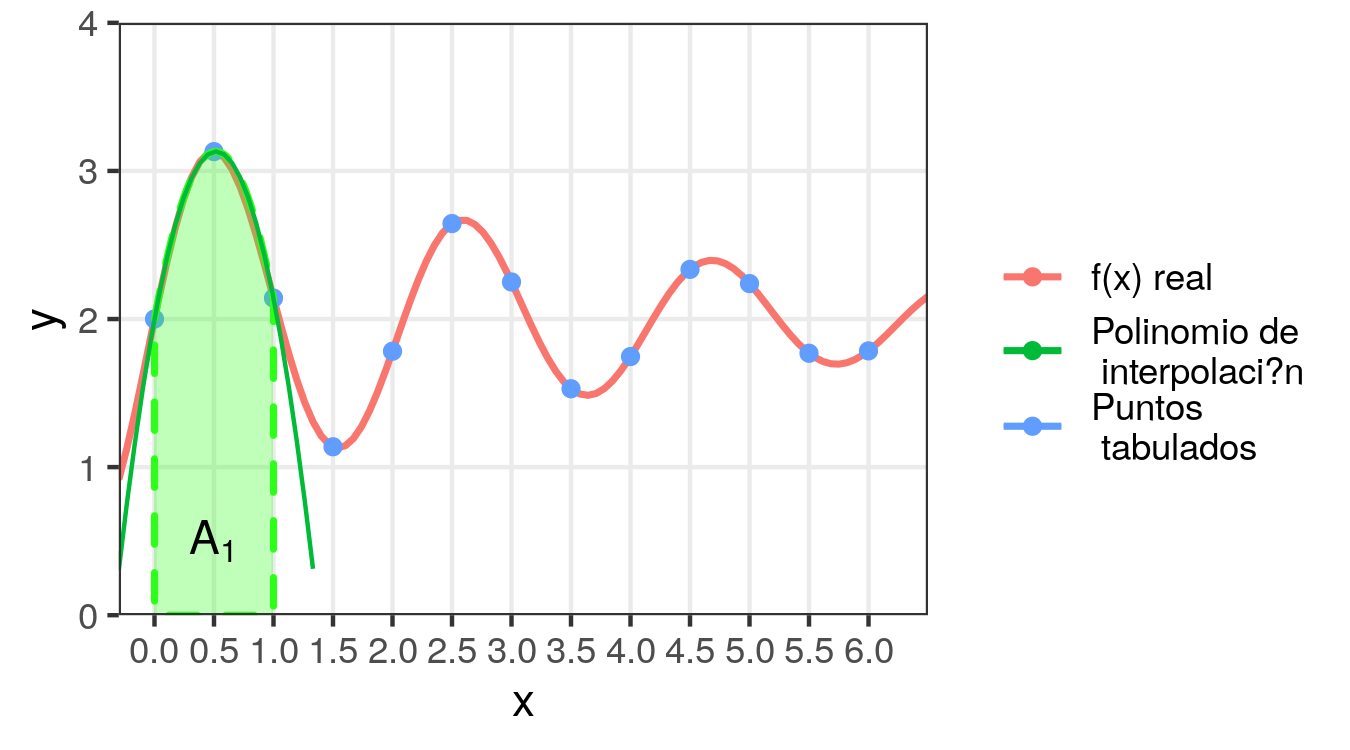
\includegraphics[width=0.95\linewidth]{Plots/U4/Unidad4_2_g5} \end{center}

\begin{itemize}
\tightlist
\item
  De manera semejante, se puede emplear la interpolación cuadrática de Newton para obtener una aproximación de la integral entre \(x_2\) y \(x_4\):
\end{itemize}

\[
\int_{x_2}^{x_4} f(x)dx \cong A_2 = \frac{h}{3} (y_2 + 4y_3 + y_4)
\]

\[A_2=1.4133\]

\begin{center}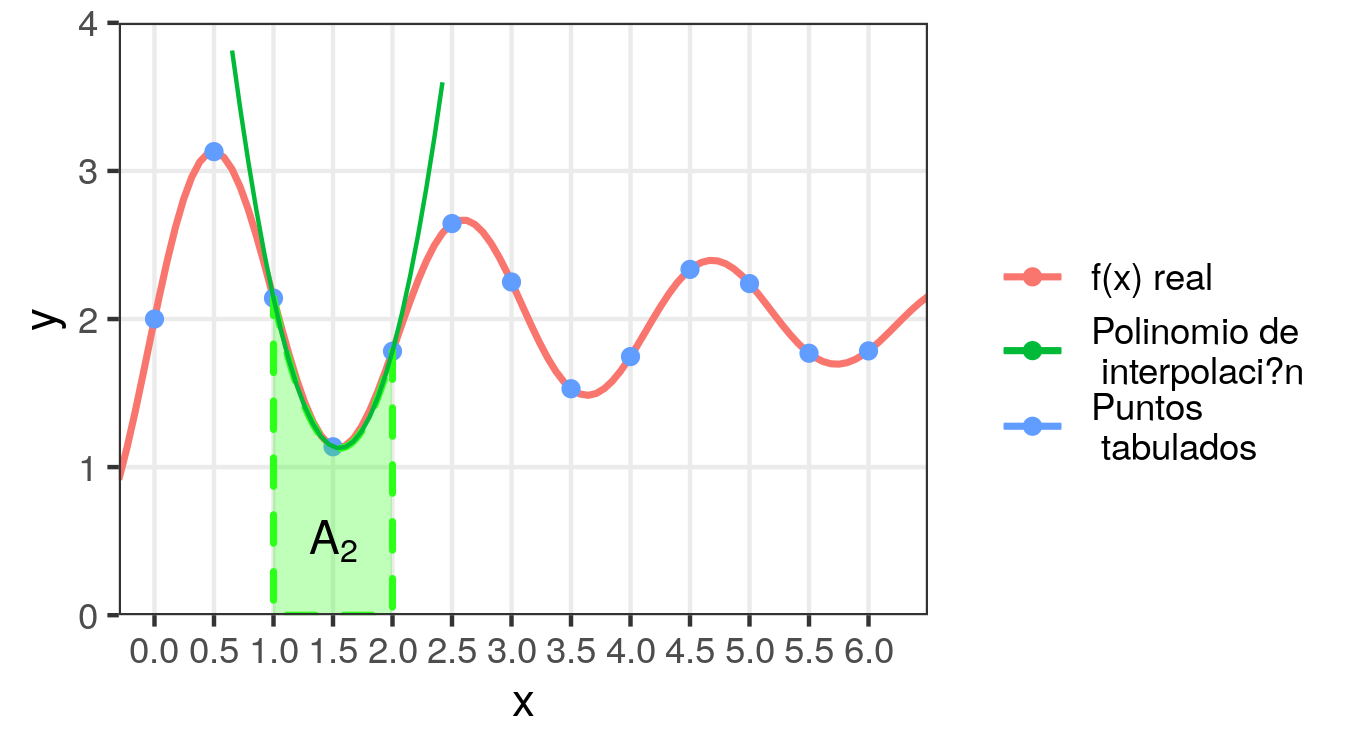
\includegraphics[width=1\linewidth]{Plots/U4/Unidad4_2_g6} \end{center}

\begin{itemize}
\tightlist
\item
  Y sucesivamente para todos los intervalos:
\end{itemize}

\[
\int_{x_{i-1}}^{x_{i+1}} f(x)dx \cong  \frac{h}{3} (y_{i-1} + 4y_i + y_{i+1}) \quad i = 1, 3, 5, \cdots, n-1
\]

\begin{itemize}
\tightlist
\item
  De modo que la suma de estas áreas resulta ser la aproximación para la integral entre \(x_0\) y \(x_n\):
\end{itemize}

\[
\int_{x_{0}}^{x_n} f(x)dx \cong \sum\limits_{\substack{i = 1\\ i~impar}}^{n-1} \frac{h}{3} (y_{i-1} + 4y_i + y_{i+1}) = \\ \frac{h}{3} \Big( y_0 + y_n + 2 \sum \limits_{\substack{i = 2\\ i~par}}^{n-2} y_i + 4 \sum\limits_{\substack{i = 1\\ i~impar}}^{n-1} y_i  \Big)
\]

\begin{itemize}
\tightlist
\item
  La fórmula hallada se conoce como \textbf{fórmula de Simpson de 1/3} y se la simboliza con:
\end{itemize}

\[
A_{1/3} = \frac{h}{3} \Big( y_0 + y_n + 2 \sum \limits_{\substack{i = 2\\ i~par}}^{n-2} y_i + 4 \sum\limits_{\substack{i = 1\\ i~impar}}^{n-1} y_i  \Big)
\]

\begin{itemize}
\item
  Para poder aplicarla, es necesario que la cantidad de puntos tabulados sea impar, es decir que la tabla tenga una cantidad par de intervalos.
\item
  Gráficamente:
\end{itemize}

\begin{center}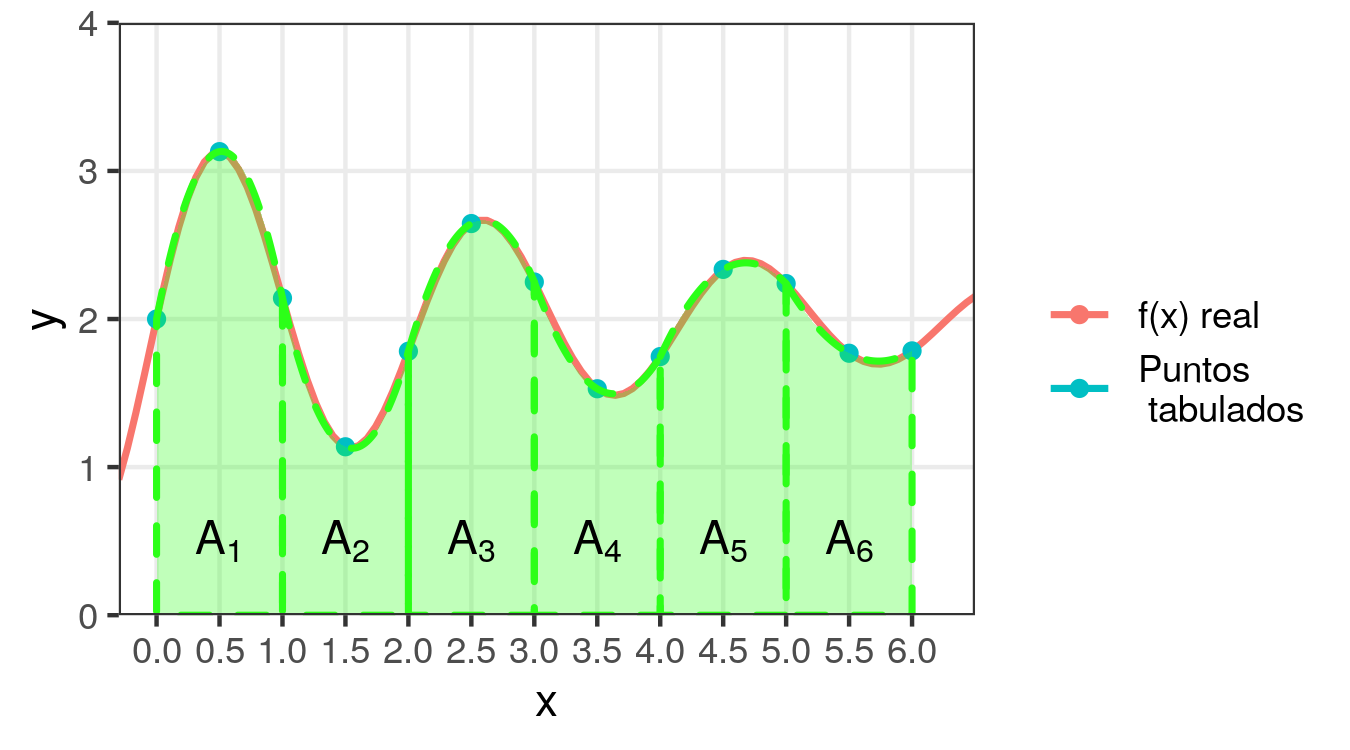
\includegraphics[width=0.85\linewidth]{Plots/U4/Unidad4_2_g7} \end{center}

\begin{itemize}
\tightlist
\item
  En el ejemplo: \(A_{1/3} = 12.3833\).
\item
  El valor exacto es: \(\int_0^{6}f(x)dx = 12.2935\), con lo cual el error relativo de la aproximación con la fórmula trapecial fue: \(7.3\%\).
\end{itemize}

\hypertarget{fuxf3rmula-de-simpson-de-38}{%
\subsection{Fórmula de Simpson de 3/8}\label{fuxf3rmula-de-simpson-de-38}}

\begin{itemize}
\tightlist
\item
  Si la interpolación es de tercer orden y la integral sólo se calcula entre los 4 primeros valores de \(x\), se obtiene:
\end{itemize}

\[
\hspace{-.25cm}
\begin{aligned}
\int_{x_0}^{x_3} f(x)dx &\cong  \int_{0}^{3} \Big[ y_0 + k \Delta y_0 + \Big( \frac{k^2}{2} - \frac{k}{2} \Big) \Delta^2 y_0  + \Big( \frac{k^3}{6} - \frac{k^2}{2} + \frac{k}{3} \Big) \Delta^3 y_0
\Big]  hdk \\
&= h \left. \Big[ y_0 k + \frac{k^2}{2} \Delta y_0  + \Big( \frac{k^3}{6} - \frac{k^2}{4} \Big) \Delta^2 y_0 + \Big( \frac{k^4}{24} - \frac{k^3}{6} + \frac{k^2}{6} \Big) \Delta^3 y_0 \Big] \right\vert_{0}^{3} \\
&= h \Big[ 3y_0 + \frac{9}{2} \Delta y_0  + \frac{9}{4} \Delta^2 y_0 + \frac{3}{8} \Delta^3 y_0\Big]
\end{aligned}
\]

\begin{itemize}
\tightlist
\item
  Dado que \(\Delta y_0 = y_1 - y_0\), \(\Delta^2 y_0 = \Delta y_1 - \Delta y_0 = y_2 - 2y_1 + y_0\), y \(\Delta^3 y_0 = \Delta^2 y_1 - \Delta^2 y_0 = y_3 - 3y_2 - 3y_1 + y_0\) nos queda:
\end{itemize}

\[
\begin{aligned}
\int_{x_0}^{x_3} f(x)dx &\cong \frac{3}{8} h (y_0 + 3y_1 + 3y_2+y_3)
\end{aligned}
\]

\begin{itemize}
\tightlist
\item
  Geométricamente, esto equivale al área \(A_1\) encerrada entre el eje de las abscisas, \(x_0\) y \(x_3\) y el polinomio integrador que pasa por \((x_0, y_0)\), \((x_1, y_1)\), \((x_2, y_2)\) y \((x_3, y_3)\):
\end{itemize}

\[A_1 = 3.5531\]

\begin{center}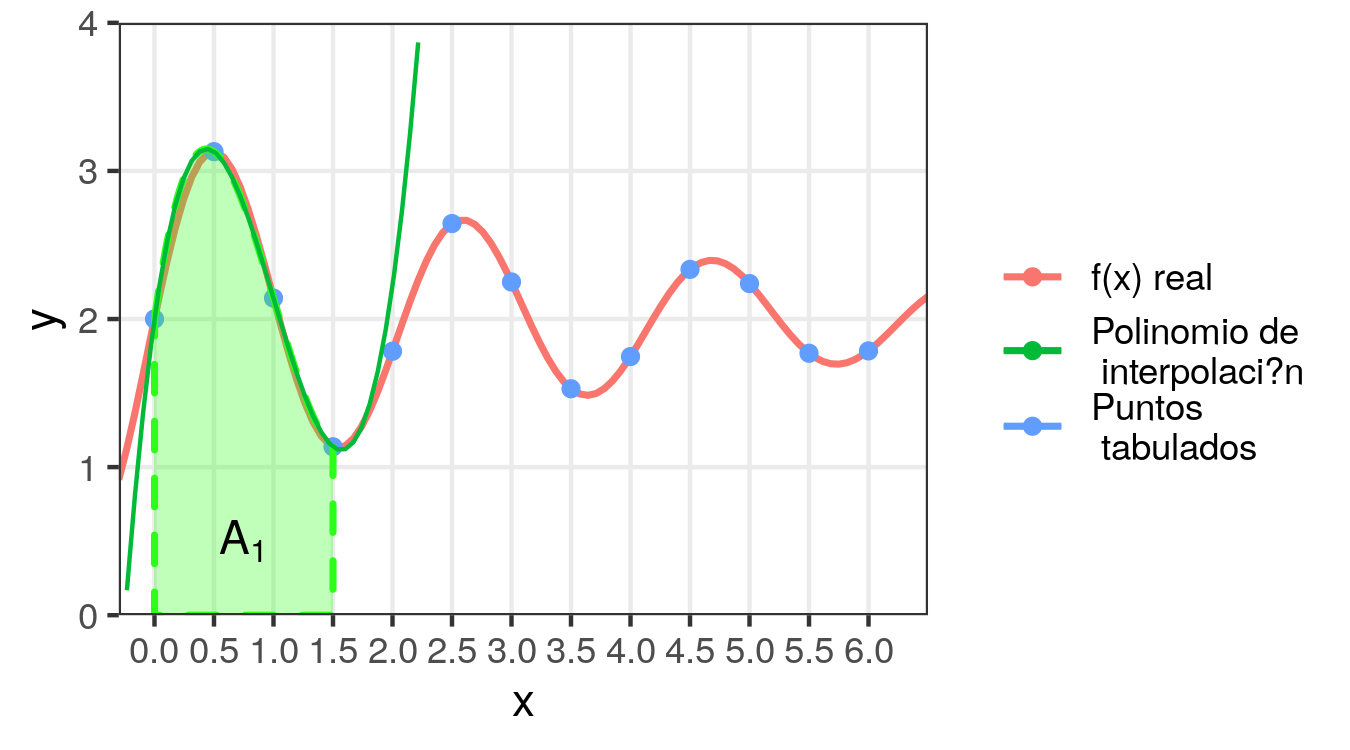
\includegraphics[width=1\linewidth]{Plots/U4/Unidad4_2_g8} \end{center}

\begin{itemize}
\tightlist
\item
  De manera semejante, se puede emplear la interpolación cúbica de Newton para obtener una aproximación de la integral entre \(x_3\) y \(x_6\):
\end{itemize}

\[
\int_{x_3}^{x_6} f(x)dx \cong A_2 = \frac{3}{8} h (y_3 + 3y_4 + 3y_5 + y_6)
\]

\[A_1 = 3.1219\]

\begin{center}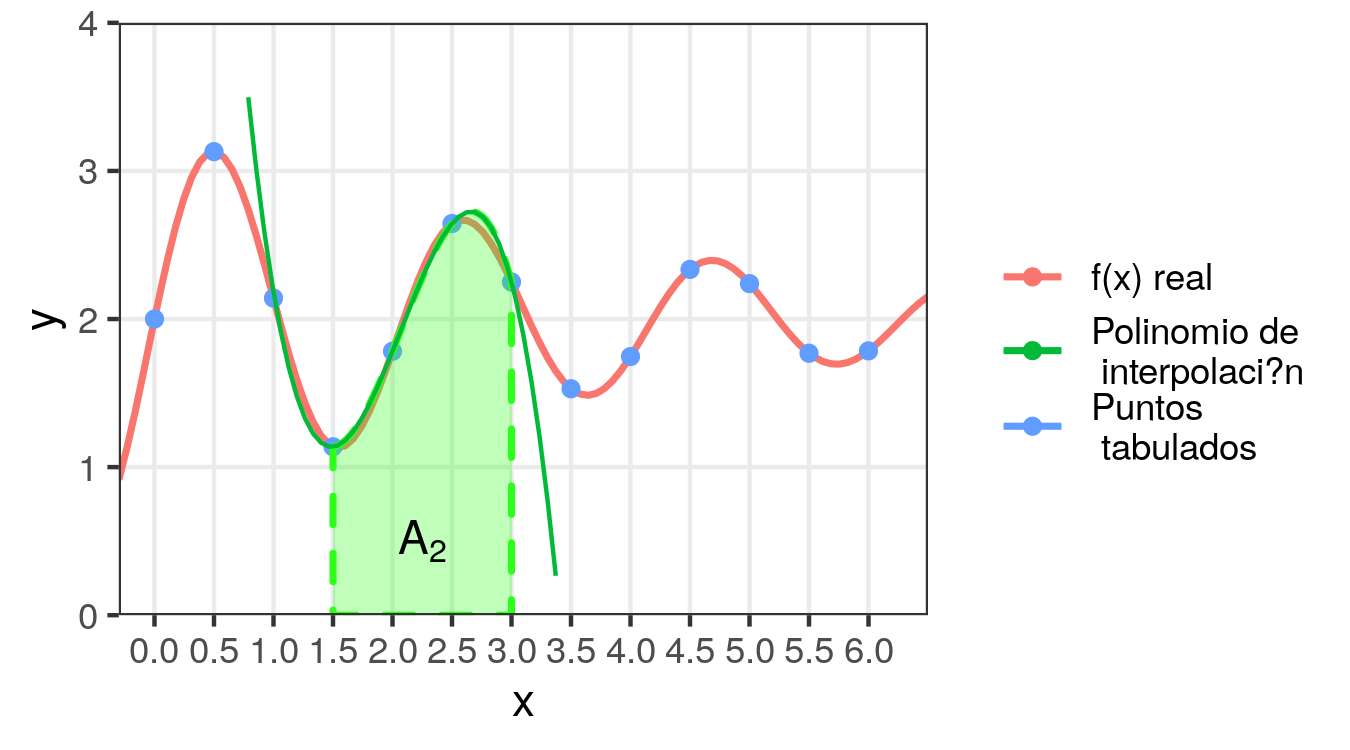
\includegraphics[width=1\linewidth]{Plots/U4/Unidad4_2_g9} \end{center}

\begin{itemize}
\tightlist
\item
  Y sucesivamente para todos los intervalos:
\end{itemize}

\[
\int_{x_{i}}^{x_{i+3}} f(x)dx \cong  \frac{3}{8} h (y_{i} + 3y_{i+1} + 3y_{i+2} + y_{i+3}) \quad i = 0, 3, 6, \cdots, n-3
\]

\begin{itemize}
\tightlist
\item
  De modo que la suma de estas áreas resulta ser la aproximación para la integral entre \(x_0\) y \(x_n\):
\end{itemize}

\[
\begin{aligned}
\int_{x_{0}}^{x_n} f(x)dx & \cong \sum\limits_{\substack{i = 0\\ ó~i~múltiplo~de~3}}^{n-3} \frac{3}{8} h (y_{i} + 3y_{i+1} + 3y_{i+2} + y_{i+3}) \\
 &= \frac{3}{8} h \Big( y_0 + y_n + 2 \sum \limits_{\substack{i = 3\\ i~múltiplo~de~3}}^{n-3} y_i + 3 \sum\limits_{\substack{i = 1\\ i~no~múltiplo~de~3}}^{n-1} y_i  \Big)
 \end{aligned}
\]

\begin{itemize}
\tightlist
\item
  La fórmula hallada se conoce como \textbf{fórmula de Simpson de 3/8} y se la simboliza con:
\end{itemize}

\[
A_{3/8} = \frac{3}{8} h \Big( y_0 + y_n + 2 \sum \limits_{\substack{i = 3\\ i~múltiplo~de~3}}^{n-3} y_i + 3 \sum\limits_{\substack{i = 1\\ i~no~múltiplo~de~3}}^{n-1} y_i  \Big)
\]

\begin{itemize}
\item
  Para poder aplicarla, es necesario que la cantidad de intervalos en la tabla sea múltiplo de 3.
\item
  Gráficamente:
\end{itemize}

\begin{center}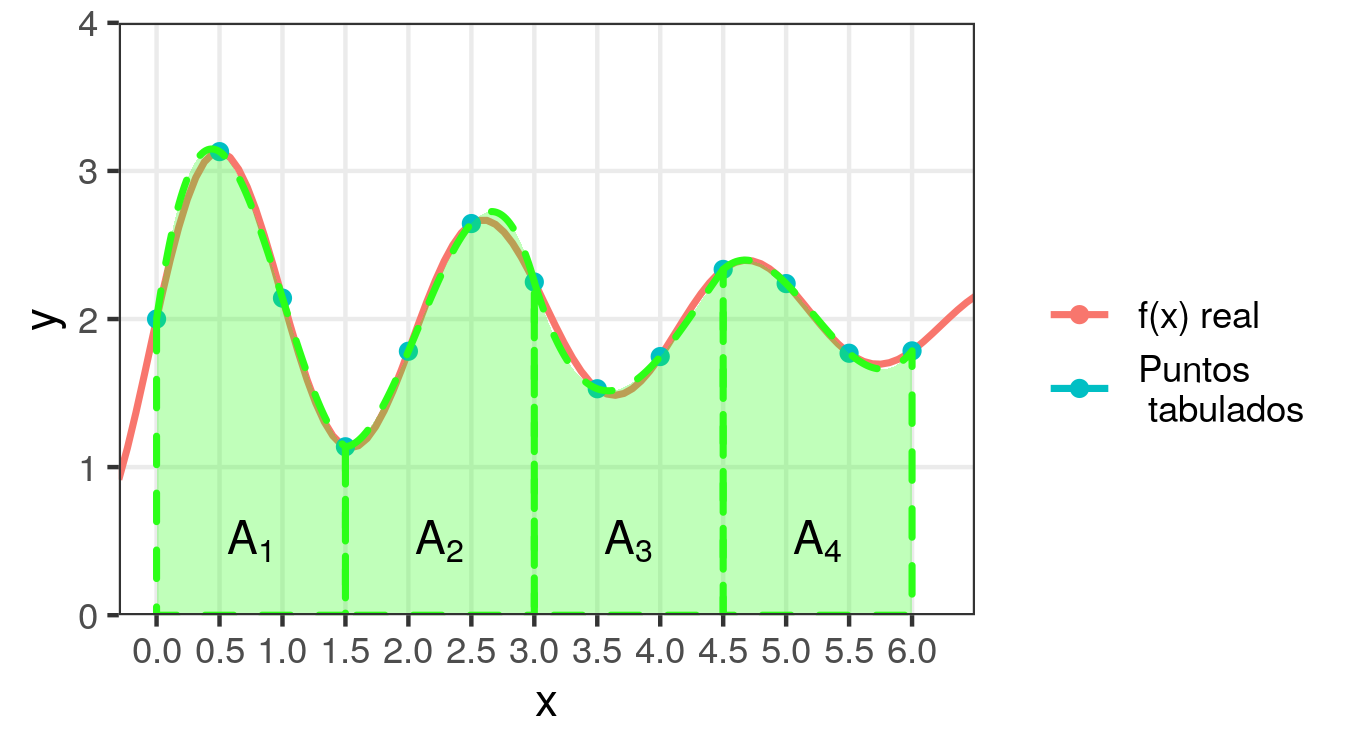
\includegraphics[width=0.85\linewidth]{Plots/U4/Unidad4_2_g10} \end{center}

\begin{itemize}
\tightlist
\item
  En el ejemplo: \(A_{3/8} = 12.4088\).
\item
  El valor exacto es: \(\int_0^{6}f(x)dx = 12.2935\), con lo cual el error relativo de la aproximación con la fórmula trapecial fue: \(9.4\%\).
\end{itemize}

\hypertarget{derivaciuxf3n-numuxe9rica}{%
\section{Derivación numérica}\label{derivaciuxf3n-numuxe9rica}}

\begin{itemize}
\tightlist
\item
  Para aproximar la derivada de una función en un punto, nuevamente haremos uso del polinomio interpolador de Newton:
\end{itemize}

\[
\begin{aligned}
f(x) & \cong y_0 + k \Delta y_0 + \frac{k(k-1)}{2!}\Delta^2 y_0 + \frac{k(k-1)(k-2)}{3!}\Delta^3 y_0 + \cdots \\
&= y_0 + k \Delta y_0 + \Big( \frac{k^2}{2} - \frac{k}{2} \Big) \Delta^2 y_0 + \Big( \frac{k^3}{6} - \frac{k^2}{2} + \frac{k}{3} \Big) \Delta^3 y_0  + \cdots
\end{aligned}
\]

\begin{itemize}
\tightlist
\item
  Se debe derivar con respecto a \(x\) el miembro derecho de la expresión anterior, aplicando la Regla de la Cadena ya que \(k = (x - x_0)/h\).
\item
  Por simplicidad, lo mostraremos sólo con el polinomio interpolador cuadrático.
\item
  Aproximación de la derivada con el polinomio interpolador cuadrático de Newton:
\end{itemize}

\[
f(x)  \cong y_0 + k \Delta y_0 + \frac{k^2}{2} \Delta^2 y_0 - \frac{k}{2} \Delta^2 y_0
\]
\[
k = \frac{x-x_0}{h} \implies \frac{\partial k}{\partial x} = \frac{1}{h}
\]

\[
\begin{aligned}
f'(x) & \cong \Delta y_0 \frac{1}{h} + \Delta^2 y_0 ~k~ \frac{1}{h} - \frac{\Delta^2 y_0}{2} \frac{1}{h} \\
& = \frac{1}{h} \Big[ \Delta y_0 + \Big( k-\frac{1}{2} \Big) \Delta^2 y_0 \Big]
\end{aligned}
\]

\textbf{Retomando el Ejemplo 1 del capítulo anterior (integración)}: vamos a aproximar el valor de \(f'(3.4)\).

\begin{longtable}[]{@{}lllllll@{}}
\toprule
\(x_k\) & \(y_k\) & \(\Delta y_k\) & \(\Delta^2 y_k\) & \(\Delta^3 y_k\) & \(\Delta^4 y_k\) & \(\Delta^5 y_k\)\tabularnewline
\midrule
\endhead
2 & 0,3010 & 0,1761 & -0,0511 & 0,0230 & -0,0127 & 0,0081\tabularnewline
3 & 0,4771 & 0,1250 & -0,0281 & 0,0103 & -0,0046 & -\tabularnewline
4 & 0,6021 & 0,0969 & -0,0178 & 0,0057 & - & -\tabularnewline
5 & 0,6990 & 0,0791 & -0,0121 & - & - & -\tabularnewline
6 & 0,7781 & 0,0670 & - & - & - & -\tabularnewline
7 & 0,8451 & - & - & - & - & -\tabularnewline
\bottomrule
\end{longtable}

\begin{itemize}
    \small
    \item $x = 3,4$
    \item $x_0 = 3$
    \item $h = 1$
    \item $k = \frac{x-x_0}{h} = \frac{3.4-3}{1} = 0.4$
    \item $\Delta y_0 = 0.1250$; $\Delta^2 y_0 = -0.0281$
\end{itemize}

\[
f'(x) \cong \frac{1}{h} \Big[ \Delta y_0 + \Big( k-\frac{1}{2} \Big) \Delta^2 y_0 \Big] = 
 0.1250 + (-0.1) (-0.0281) = 0.12781
\]

Nota: esta fórmula se conoce como \emph{aproximación por diferencias hacia adelante}, pero se pueden lograr aproximaciones más precisas de otras formas, por ejemplo, haciendo que el punto de interés \(x\) esté en el centro del rango del polinomio interpolador (\emph{aproximación por diferencias centrales}).

\hypertarget{autovalores-y-autovectores}{%
\chapter{Autovalores y Autovectores}\label{autovalores-y-autovectores}}

\hypertarget{generalidades-3}{%
\section{Generalidades}\label{generalidades-3}}

\begin{itemize}
\tightlist
\item
  Los \textbf{autovalores} y \textbf{autovectores} son esas cosas raras que aparecen por todos lados pero nunca terminamos por entender.
\item
  El objetivo de esta unidad es ver métodos para su cálculo, pero antes vamos a repasar qué son (\textbf{informalmente}, \textbf{sin rigurosidad}, el que avisa no traiciona\ldots{})
\end{itemize}

\begin{itemize}
\tightlist
\item
  En muchas disciplinas los objetos que se estudian se representan con \emph{vectores} (ej. \(\textbf{x}\), \(\textbf{y}\)) y las cosas que se hacen con ellos son \emph{transformaciones lineales}, que se representan como \emph{matrices} (ej. \(\textbf{A}\)).
\item
  Así, en muchas situaciones las relaciones que importan entre esos objetos/vectores se expresan como:
\end{itemize}

\[\textbf{y} = \textbf{A} \textbf{x}\]

\begin{itemize}
\item
  Esto abarca desde sistemas de ecuaciones lineales (presentes casi en todos lados en ciencia) hasta problemas muy sofisticados en ingeniería.
\item
  Ahora bien, en general no es muy fácil mirar a la matriz \(\textbf{A}\) y directamente darse cuenta qué es lo que va a pasar cuando se la multipliquemos a \(\textbf{x}\).
\item
  Sin embargo, podríamos encontrar casos donde haya una relación muy simple entre el vector \(\textbf{x}\) y el vector resultado \(\textbf{y=Ax}\).
\item
  Por ejemplo, si miramos la matriz \(\mathbf{A} = \begin{bmatrix} 0 & 1 \\ 1 & 0 \end{bmatrix}\) y se la multiplicamos al vector \(\textbf{x} = \begin{bmatrix} 1 \\ 1 \end{bmatrix}\), ¡nos da como resultado el mismo vector \(\textbf{x}\)!
\item
  Es decir, que para ese vector, es muy fácil ver qué aspecto tiene \(\textbf{Ax}\).
\item
  Se puede generalizar esta observación con el concepto de \textbf{autovectores}.
\item
  Un \textbf{autovector} de una matriz \(\textbf{A}\) es cualquier vector \(\textbf{x}\) para el que sólo cambia su escala cuando se lo multiplica con \(\textbf{A}\), es decir: \(\textbf{Ax} = \lambda \textbf{x}\), para algún número \(\lambda\) real o complejo, que recibe el nombre de \textbf{autovalor}.
\item
  Entonces si una matriz \(\textbf{A}\) describe algún tipo de sistema, los autovectores son aquellos vectores que, cuando pasan por el sistema, se modifican en una forma muy sencilla.
\item
  Por ejemplo, si \(\textbf{A}\) describe operaciones geométricas, en principio \(\textbf{A}\) podría estirar y rotar a los vectores, sin embargo, a sus autovectores lo único que puede hacerles es estirarlos, no rotarlos.
\item
  Sea: \(\mathbf{A} = \begin{bmatrix} 3 & 2 \\ 1 & 4 \end{bmatrix}\), \(\textbf{u} = \begin{bmatrix} 1 \\ 1 \end{bmatrix}\), \(\textbf{v} = \begin{bmatrix} 1 \\ -0.5 \end{bmatrix}\) y \(\textbf{w} = \begin{bmatrix} 0 \\ 1 \end{bmatrix}\).
\item
  En este gráfico podemos ver los vectores antes de transformarlos (multiplicarlos) mediante \(\mathbf{A}\):
\end{itemize}

\begin{center}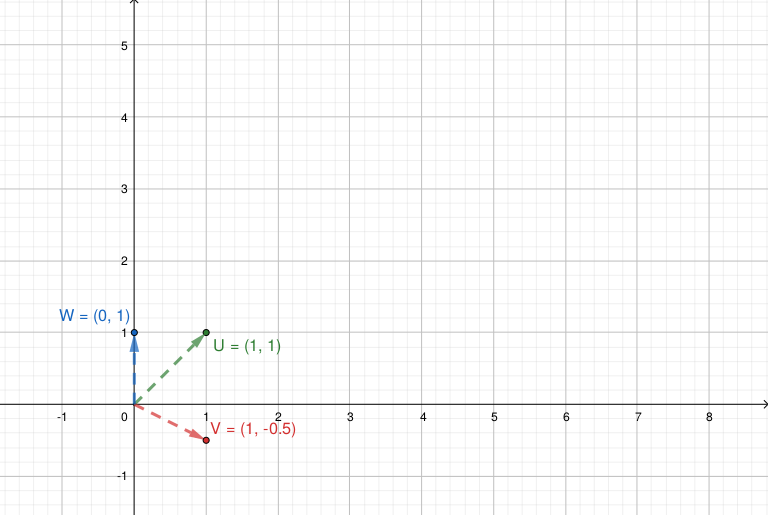
\includegraphics[width=1\linewidth]{Plots/U5/auto1} \end{center}

\begin{itemize}
\tightlist
\item
  Y en este gráfico podemos ver como quedan luego de la transformación:
\end{itemize}

\begin{center}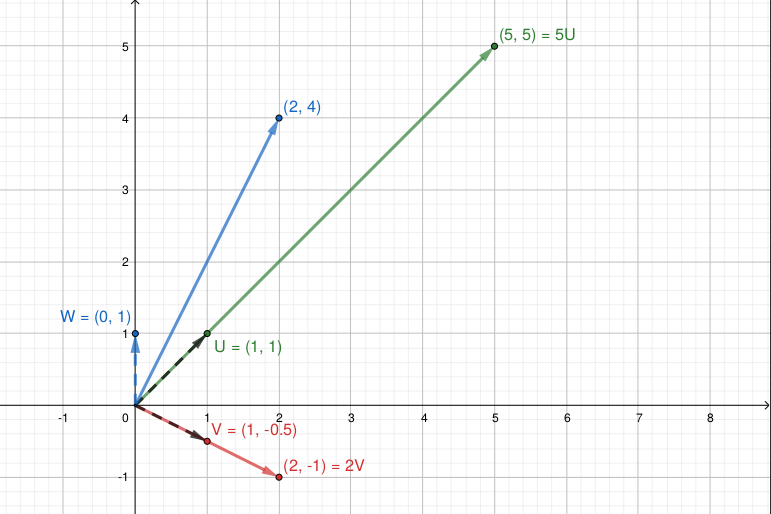
\includegraphics[width=1\linewidth]{Plots/U5/auto2} \end{center}

\begin{itemize}
\item
  \(\textbf{u}\) y \(\textbf{v}\) no cambiaron su dirección, sólo su norma: son \textbf{autovectores} de \(\textbf{A}\), asociados a los autovalores 5 y 2.
\item
  En cambio, la matriz \(\textbf{A}\) modificó la dirección de \(\textbf{w}\), entonces no es un autovector.
\end{itemize}

\hypertarget{definiciuxf3n}{%
\subsection{Definición}\label{definiciuxf3n}}

\begin{itemize}
\item
  Dada una matriz \(\textbf{A}\) cuadradada de orden \(n\), llamamos \textbf{autovector} o \textbf{vector propio} de \(\textbf{A}\) a todo vector \(\textbf{x}\) de orden \(n\) cuya dirección no se modifica al transformarlo mediante \(\textbf{A}\).

  \begin{itemize}
  \tightlist
  \item
    Transformarlo mediante \(\textbf{A}\) significa realizar el producto \(\textbf{Ax}\) dando como resultado un nuevo vector de orden \(n\).
  \item
    Que la dirección de \(\textbf{x}\) no se modifique significa que el nuevo vector debe ser múltiplo de \(\textbf{x}\), es decir, igual a \(\lambda \textbf{x}\), con \(\lambda \in \mathbb{C}\), que recibe el nombre de \textbf{autovalor} o \textbf{valor propio} de A.
  \end{itemize}
\item
  Lo anterior se resume en la siguiente expresión: \(\textbf{x}\) es un autovector y \(\lambda\) es un autovalor de \(\textbf{A}\) si:
\end{itemize}

\[\textbf{Ax} = \lambda \textbf{x}, \quad \textbf{x} \neq \textbf{0}, \quad \lambda \in \mathbb{C}\]

\textbf{Observación}

\begin{itemize}
\tightlist
\item
  Se debe observar que si \(\textbf{x}\) es un autovector con el autovalor \(\lambda\) entonces cualquier múltiplo diferente de cero de \(\textbf{x}\) es también un autovector con el autovalor \(\lambda\).
\end{itemize}

\hypertarget{propiedades}{%
\subsection{Propiedades}\label{propiedades}}

\begin{itemize}
\item
  Dada una matriz \(\textbf{A}\) cuadradada de orden \(n\):

  \begin{itemize}
  \tightlist
  \item
    \(\textbf{A}\) tiene \(n\) autovalores, \(\lambda_1, \lambda_2, \cdots, \lambda_n\), los cuales no necesariamente son todos distintos.
  \item
    \(tr(A) = \sum_{i=1}^n a_{ii} = \sum_{i=1}^n \lambda_{i}\).
  \item
    \(\det(A) = \prod_{i=1}^n \lambda_{i}\).
  \item
    Los autovalores de \(\textbf{A}^k\) son \(\lambda_1^k, \lambda_2^k, \cdots, \lambda_n^k\).
  \item
    Si \(\textbf{A}\) es real y simétrica todos sus autovalores son reales y los autovectores correspondientes a distintos autovalores son ortogonales.
  \item
    Si \(\textbf{A}\) es triangular los valores propios son los elementos diagonales.
  \item
    Los autovalores de una matriz y su transpuesta son los mismos.
  \item
    Si \(\textbf{A}\) tiene inversa, los autovalores de \(\textbf{A}^{-1}\) son \(1/\lambda_1, 1/\lambda_2, \cdots, 1/\lambda_n\).
  \item
    Los valores de \(\alpha \textbf{A}\) son \(\alpha \lambda_1, \alpha \lambda_2, \cdots, \alpha \lambda_n, \, \alpha \in \mathbb{R}\).
  \item
    Las matrices \(\textbf{A}\) y \(\textbf{Q}^{-1}\textbf{AQ}\) (forma cuadrática) tienen los mismos valores propios.
  \end{itemize}
\end{itemize}

\hypertarget{obtenciuxf3n-los-autovalores-y-autovectores}{%
\section{Obtención los autovalores y autovectores}\label{obtenciuxf3n-los-autovalores-y-autovectores}}

\begin{itemize}
\tightlist
\item
  A partir de la expresión anterior:
\end{itemize}

\[
\textbf{Ax} = \lambda \textbf{x} \implies \textbf{Ax} - \lambda \textbf{x} = \textbf{0} \implies (\textbf{A} - \lambda \textbf{I}) \textbf{x} = \textbf{0} 
\]

\begin{itemize}
\tightlist
\item
  Esto es un sistema de ecuaciones lineales con matriz de coeficientes \(\textbf{A} - \lambda \textbf{I}\) y vector de términos independientes \(\textbf{0}\), es decir, es un \textbf{sistema homogéneo} y como tal tiene solución no nula si: \(\det (\textbf{A} - \lambda \textbf{I}) = 0\) (repasar por qué).
\end{itemize}

\begin{itemize}
\tightlist
\item
  El desarrollo de esta expresión conduce a un polinomio de grado \(n\) en la incógnita \(\lambda\) que igualado a cero es llamado \textbf{ecuación característica} y su resolución permite hallar los autovalores.
\end{itemize}

\textbf{Ejemplo}

\begin{gather*}
\mathbf{A} = 
\begin{bmatrix} 
    5 & -2 & 0 \\ 
    -2 & 3 & -1 \\
    0 & -1 & 1    
\end{bmatrix} 
\implies \\ \\
 det(\textbf{A} - \lambda \textbf{I}) = 
\begin{vmatrix}
    5 - \lambda & -2 & 0 \\ 
    -2 & 3 - \lambda & -1 \\
    0 & -1 & 1-\lambda
\end{vmatrix}  = 
\cdots  = -\lambda^3 + 9 \lambda^2 - 18 \lambda + 6 = 0
\end{gather*}

\begin{itemize}
\item
  Las soluciones de la ecuación característica son \(\lambda_1 = 6.2899, \lambda_2 = 2.2943\) y \(\lambda_3 = 0.4158\), los cuales son los autovalores de \(\textbf{A}\).
\item
  Hallar la ecuación característica ya es demasiado trabajoso para \(n=3\), y mucho más será para mayor \(n\)\ldots{} por eso veremos métodos que directamente nos den los coeficientes de esta ecuación.
\item
  Pero nos faltan los autovectores!
\item
  Para eso hacemos uso de la definición: \(\textbf{A}\) es un autovector de \(\textbf{A}\) asociado al autovalor \(\lambda\) si \((\textbf{A} - \lambda \textbf{I}) \textbf{x} = \textbf{0}\).
\item
  Tomamos uno de los autovalores, por ejemplo, \(\lambda_1 = 6.2899\) y resolvemos el sistema de ecuaciones que la expresión anterior plantea:
\end{itemize}

\begin{gather*}
(\textbf{A} - 6.2899 \, \textbf{I}) \textbf{x} = \textbf{0} \implies 
\begin{bmatrix}
    -1.2899 & -2 & 0 \\ 
    -2 & -3.2899 & -1 \\
    0 & -1 & -5.2899
\end{bmatrix}
\begin{bmatrix}
    x_1 \\ x_2 \\ x_3
\end{bmatrix} 
=
\begin{bmatrix}
    0 \\ 0 \\ 0
\end{bmatrix}
\\ \\
\implies
\begin{cases}
-1.2899 x_1 -2 x_2 &= 0 \\
-2 x_1 - 3.2899 x_2 - x_3 &= 0\\
-x_2 - 5.2899 x_3 &= 0
\end{cases} \implies
\begin{cases}
    x_1 = 8.2018 x_3\\
    x_2 = -5.2899 x_2\\
    x_3 \in \mathbb{R} 
\end{cases}
\end{gather*}

\begin{itemize}
\tightlist
\item
  Como se puede ver la solución de este sistema homogéneo no es única, representando los infinitos autovectores asociados a \(\lambda_1 = 6.2899\). Por ejemplo, si elegimos \(x_3 = 1\), obtenemos el autovector:
\end{itemize}

\[
\textbf{x}_1 = 
\begin{bmatrix}
    8.2018 \\ -5.2899 \\ 1
\end{bmatrix} 
\]

\begin{itemize}
\tightlist
\item
  En general, se resuelve informando el autovector de norma 1 que sí es único.
\item
  De la misma forma se procede con los restantes autovalores \(\lambda_2\) y \(\lambda_3\).
\end{itemize}

\hypertarget{resumen-1-obtener-autovalores-y-autovectores}{%
\subsection{Resumen 1: Obtener autovalores y autovectores}\label{resumen-1-obtener-autovalores-y-autovectores}}

\begin{itemize}
\tightlist
\item
  \textbf{Paso 1}: desarrollar la expresión de \(\det(\textbf{A} - \lambda \textbf{I})\) para obtener la ecuación característica (muy engorroso para n \textgreater{} 3):
\end{itemize}

\[
f(\lambda) = \det(\textbf{A} - \lambda \textbf{I}) = \lambda^n + b_1 \lambda^{n-1} + \cdots + b_{n-1} \lambda + b_n = 0
\]

\begin{itemize}
\item
  \textbf{Paso 2}: resolver la ecuación característica para hallar los autovalores \(\lambda_1, \lambda_2, \cdots, \lambda_n\). Dependiendo de \(n\), podemos hacerlo a mano, con la calculadora o con los métodos de la Unidad 2.
\item
  \textbf{Paso 3}: tomar cada autovalor \(\lambda_i\) y resolver el sistema de ecuaciones lineales \((\textbf{A} - \lambda_i \textbf{I}) \textbf{x} = \textbf{0}\). No nos sirven los métodos de la Unidad 3 porque este sistema es compatible indeterminado, realizarlo ``a mano'' y dar un expresión para los infinitos autovectores o informar el autovector de norma 1.
\end{itemize}

\hypertarget{muxe9todo-de-krylov}{%
\section{Método de Krylov}\label{muxe9todo-de-krylov}}

\begin{itemize}
\item
  Como ya mencionamos, el desarrollo de \(\det(\textbf{A} - \lambda \textbf{I})\) para obtener la ecuación característica tal como lo vimos en el ejemplo inicial se vuelve engorroso rápidamente.
\item
  El método de Krylov permite obtenerla de manera sencilla, basándose en el siguiente teorema:
\item
  \textbf{Teorema de Caylay-Hamilton}: toda matriz cuadrada \(\textbf{A}\) verifica su propia ecuación característica. Es decir, siendo la ecuación característica:
\end{itemize}

\[
f(\lambda) = \det(\textbf{A} - \lambda \textbf{I}) = \lambda^n + b_1 \lambda^{n-1} + \cdots + b_{n-1} \lambda + b_n = 0,
\]

se verifica que:

\[
f(\textbf{A}) = \textbf{A}^n + b_1 \textbf{A}^{n-1} + \cdots + b_{n-1} \textbf{A} + b_n \textbf{I} = \textbf{0}_{n\times n}
\]

\textbf{Ejemplo}

\begin{gather*}
\small
\mathbf{A} = 
\begin{bmatrix} 
    5 & -2 & 0 \\ 
    -2 & 3 & -1 \\
    0 & -1 & 1    
\end{bmatrix}
\\ \\
\mathbf{A}^2 = 
\begin{bmatrix} 
    29 & -16 & 2 \\ 
    -16 & 14 & -4 \\
    2 & -1 & 1    
\end{bmatrix}
\\ \\
\mathbf{A}^3 = 
\begin{bmatrix} 
    177 & -108 & 18 \\ 
    -108 & 78 & -18 \\
    18 & -18 & 6    
\end{bmatrix} \\ \\
f(\textbf{A}) = f(\textbf{A}) = 
   = \textbf{A}^3 + b_1 \textbf{A}^{2} +  b_{2} \textbf{A} + b_3 \textbf{I} 
   = \textbf{0} \implies \\ \\
\begin{bmatrix} 
    177 & -108 & 18 \\ 
    -108 & 78 & -18 \\
    18 & -18 & 6    
\end{bmatrix}
+ b_1
\begin{bmatrix} 
    29 & -16 & 2 \\ 
    -16 & 14 & -4 \\
    2 & -1 & 1    
\end{bmatrix}
+ b_2
\begin{bmatrix} 
    5 & -2 & 0 \\ 
    -2 & 3 & -1 \\
    0 & -1 & 1    
\end{bmatrix}  \\ \\
+ b_3
\begin{bmatrix} 
    1 & 0 & 0 \\ 
    0 & 1 & 0 \\
    0 & 0 & 1    
\end{bmatrix} =
\begin{bmatrix} 
    0 & 0 & 0 \\ 
    0 & 0 & 0 \\
    0 & 0 & 0    
\end{bmatrix}
\implies \\ \\
\begin{bmatrix}        
    177 + 29 b_1 + 5 b_2 + b_3 &   -108-16  b_1 -2  b_2       &  18 +2  b_1              \\ 
    -108 -16  b_1 -2  b_2      &  78  + 14 b_1 + 3 b_2 + b_3  &   -18 -4  b_1 -  b_2     \\
    18+2  b_1                  &   -18 -4  b_1 -1  b_2        &   6 + 2 b_1   b_2 + b_3
\end{bmatrix} =
\begin{bmatrix} 
    0 & 0 & 0 \\ 
    0 & 0 & 0 \\
    0 & 0 & 0    
\end{bmatrix}
\end{gather*}

\begin{itemize}
\item
  Cualquiera de las columnas constituyen un sistema de tres ecuaciones lineales en las incógnitas \(b_1, b_2\) y \(b_3\), los coeficientes de la ecuación característica.
\item
  Podemos usar el siguiente artificio para generar un único sistema de ecuaciones:
\end{itemize}

\[
f(\textbf{A}_{n\times n}) = \textbf{0}_{n\times n} \implies f(\textbf{A})  \, \textbf{y}= \textbf{0}\, \textbf{y}  = \textbf{0}_{n\times 1}  \quad \forall \, \textbf{y}_{n\times 1} \in \mathbb{R}^n
\]

\begin{itemize}
\tightlist
\item
  Por ejemplo, tomando \(\textbf{y} = [1 \quad 0 \quad 0]^t\), nos queda:
\end{itemize}

\begin{gather*}
f(\textbf{A})  \, \textbf{y} = \textbf{0} \, \textbf{y}  \\ \\
\implies (\textbf{A}^3 + b_1 \textbf{A}^2 + b_{2} \textbf{A} + b_3 \textbf{I})  \textbf{y} = \textbf{0} \\ \\
\implies \textbf{A}^3 \textbf{y} + b_1 \textbf{A}^{2} \textbf{y} + b_{2} \textbf{A} \textbf{y} + b_3 \textbf{y} = \textbf{0} \\ \\
\implies
\begin{bmatrix} 
    177 & -108 & 18 \\ 
    -108 & 78 & -18 \\
    18 & -18 & 6    
\end{bmatrix}
\begin{bmatrix} 1 \\ 0 \\ 0 \end{bmatrix}
+ b_1
\begin{bmatrix} 
    29 & -16 & 2 \\ 
    -16 & 14 & -4 \\
    2 & -1 & 1    
\end{bmatrix}
\begin{bmatrix} 1 \\ 0 \\ 0 \end{bmatrix} + \\ \\
+ b_2
\begin{bmatrix} 
    5 & -2 & 0 \\ 
    -2 & 3 & -1 \\
    0 & -1 & 1    
\end{bmatrix} 
\begin{bmatrix} 1 \\ 0 \\ 0 \end{bmatrix} + 
b_3
\begin{bmatrix} 
    1 & 0 & 0 \\ 
    0 & 1 & 0 \\
    0 & 0 & 1    
\end{bmatrix}
\begin{bmatrix} 1 \\ 0 \\ 0 \end{bmatrix} =
\begin{bmatrix} 0 \\ 0 \\ 0 \end{bmatrix} \\ \\
\implies
\begin{bmatrix} 177 \\ -108 \\ 18 \end{bmatrix}
+ b_1
\begin{bmatrix} 29 \\ -16 \\ 2 \end{bmatrix}
+ b_2
\begin{bmatrix} 5 \\ -2 \\ 0 \end{bmatrix} 
+ b_3
\begin{bmatrix} 1 \\ 0 \\ 0 \end{bmatrix} =
\begin{bmatrix} 0 \\ 0 \\ 0 \end{bmatrix} \\ \\
\implies
\begin{bmatrix} 
    29 & 5 & 1 \\ 
    -16 & -2 & 0 \\
    2 & 0 & 0    
\end{bmatrix}
\begin{bmatrix} b_1 \\ b_2 \\ b_3 \end{bmatrix} =
\begin{bmatrix} -177 \\ 108 \\ -18 \end{bmatrix}
\end{gather*}

\begin{itemize}
\item
  Lo anterior no es más que un sistema de tres ecuaciones lineales, \(\mathbf{Cb=d}\), donde:

  \begin{itemize}
  \tightlist
  \item
    el vector incógnitas es \(\mathbf{b} = \begin{bmatrix} b_1 \\ b_2 \\ b_3 \end{bmatrix}\), los coeficientes de la ecuación característica.
  \item
    el vector de términos independientes es \(\mathbf{d} = - \mathbf{A}^3 \, \mathbf{y} = \begin{bmatrix} -177 \\ 108 \\ -18 \end{bmatrix}\).
  \item
    la matriz de coeficientes es \(\mathbf{C} = [\mathbf{A}^{2} \, \mathbf{y} \quad \mathbf{A} \, \mathbf{y} \quad \mathbf{y}] = \begin{bmatrix} 29 & 5 & 1 \\ -16 & -2 & 0 \\2 & 0 & 0 \end{bmatrix}\)
  \end{itemize}
\item
  Dependiendo de \(n\), podemos resolver este sistema ``a mano'', con la calcu o con algunos de los métodos de la Unidad 3.
\item
  En el ejemplo, el resultado es: \(b_1 = -9, b_2 = 18\) y \(b_3 = -6\).
\item
  La ecuación característica entonces es:
\end{itemize}

\[
\lambda^3 - 9 \lambda^2 + 18 \lambda - 6 = 0
\]

\begin{itemize}
\tightlist
\item
  Esta ecuación coincide con la que obtuvimos en la sección anterior.
\item
  A partir de aquí, se debe continuar desde el Paso 2 del Resumen 1 para hallar los autovalores y sus respectivos autovectores.
\end{itemize}

\hypertarget{resumen-2-muxe9todo-de-krylov}{%
\subsection{Resumen 2: Método de Krylov}\label{resumen-2-muxe9todo-de-krylov}}

\begin{itemize}
\tightlist
\item
  \textbf{Qué necesita}: la matriz \(\mathbf{A}\) y un vector \(\mathbf{y}\).
\item
  \textbf{Qué nos da}: un sistema de ecuaciones para obtener los coeficientes de la ecuación característica.
\item
  \textbf{Paso 1}: elegir un vector \(\mathbf{y}\) de dimensión \(n \times 1\).
\item
  \textbf{Paso 2}: crear la matriz de coeficientes \(\mathbf{C} = [\mathbf{A}^{n-1} \, \mathbf{y} \quad \cdots \quad \mathbf{A}^2 \, \mathbf{y} \quad \mathbf{A} \, \mathbf{y} \quad \mathbf{y}]\).
\item
  \textbf{Paso 3}: crear el vector de términos independientes \(\mathbf{d} = - \mathbf{A}^n \, \mathbf{y}\), de dimensión \(n \times 1\).
\item
  \textbf{Paso 4}: resolver el sistema \(\mathbf{Cb=d}\), donde el vector de incógnitas \(\mathbf{b}\) son los coeficientes de la ecuación característica.
\item
  \textbf{Paso 5}: formar la ecuación característica y continuar desde el Paso 2 del Resumen 1 para hallar los autovalores y sus respectivos autovectores.
\end{itemize}

\hypertarget{muxe9todo-de-faddeev-leverrier}{%
\section{Método de Faddeev-LeVerrier}\label{muxe9todo-de-faddeev-leverrier}}

\begin{itemize}
\tightlist
\item
  Este método propone hallar los coeficientes \(b_k\) de la ecuación característica:
\end{itemize}

\[
f(\lambda) = \det(\textbf{A} - \lambda \textbf{I}) = \lambda^n + b_1 \lambda^{n-1} + \cdots + b_{n-1} \lambda + b_n = 0
\]

mediante el siguiente cálculo iterativo:

\begin{gather*}
\textbf{M}_1 = \textbf{A} \qquad b_1 = - tr(\textbf{M}_1) \\
\textbf{M}_k = \textbf{A} (\textbf{M}_{k-1} + b_{k-1} \textbf{I}) \qquad b_k = - \frac{tr(\textbf{M}_k)}{k} \qquad k = 2, 3, \cdots, n\\
\end{gather*}

\begin{itemize}
\item
  Este método se deriva a partir de propiedades de matrices conjugadas.
\item
  En nuestro ejemplo, tenemos:
\end{itemize}

\begin{gather*}
\textbf{M}_1 = \textbf{A} = 
\begin{bmatrix} 
    5 & -2 & 0 \\ 
    -2 & 3 & -1 \\
    0 & -1 & 1  
\end{bmatrix} 
\qquad b_1 = - tr(\textbf{M}_1) = -9 \\
\textbf{M}_2 = \textbf{A} (\textbf{M}_{1} + b_{1} \textbf{I}) = 
\begin{bmatrix} 
    -16 & 2 & 2 \\ 
    2 & -13 & 5 \\
    2 & 5 & -7  
\end{bmatrix} 
\qquad b_2 = - \frac{tr(\textbf{M}_2)}{2} = 18\\
\textbf{M}_3 = \textbf{A} (\textbf{M}_{2} + b_{2} \textbf{I}) = 
\begin{bmatrix} 
    6 & 0 & 0 \\ 
    0 & 6 & 0 \\
    0 & 0 & 6  
\end{bmatrix} 
\qquad b_3 = - \frac{tr(\textbf{M}_3)}{3} = -6\\
\end{gather*}

\begin{itemize}
\tightlist
\item
  La ecuación característica entonces es:
\end{itemize}

\[
\lambda^3 - 9 \lambda^2 + 18 \lambda - 6 = 0
\]

\begin{itemize}
\item
  A partir de aquí, otra vez se debe continuar desde el Paso 2 del Resumen 1 para hallar los autovalores y sus respectivos autovectores.
\item
  Este método también sirve para calcular \(\textbf{A}^{-1}\).
\item
  Por Cayley-Hamilton, ya sabemos que:
\end{itemize}

\[
f(\textbf{A}) = \textbf{A}^n + b_1 \textbf{A}^{n-1}  + \cdots + b_{n-2} \textbf{A}^2  + b_{n-1} \textbf{A} + b_n \textbf{I} = \textbf{0}
\]

\begin{itemize}
\tightlist
\item
  Premultiplicando por \(\textbf{A}^{-1}\) nos queda:
\end{itemize}

\begin{gather*}
\textbf{A}^{-1} (\textbf{A}^n + b_1 \textbf{A}^{n-1} + \cdots + b_{n-2} \textbf{A}^2 + b_{n-1} \textbf{A} + b_n \textbf{I}) = \textbf{A}^{-1} \, \textbf{0} \\
\textbf{A}^{n-1} + b_1 \textbf{A}^{n-2} + \cdots + b_{n-2} \textbf{A} +b_{n-1} \textbf{I} + b_n \textbf{A}^{-1} = \textbf{0} \\
\textbf{A}^{-1} = - \frac{1}{b_n} \Big( \textbf{A}^{n-1} + b_1 \textbf{A}^{n-2} + \cdots + b_{n-2} \textbf{A} + b_{n-1} \textbf{I} \Big) \\
\textbf{A}^{-1} = - \frac{1}{b_n} \Big( \textbf{M}_{n-1} + b_{n-1} \textbf{I}  \Big) \\
\end{gather*}

\ldots{} donde el último reemplazo se deduce a partir de la fórmula iterativa vista antes:

\[
\begin{aligned}
\textbf{M}_1 &= \textbf{A}\\
\textbf{M}_2 &= \textbf{A} (\textbf{M}_{1} + b_{1} \textbf{I})  = \textbf{A} (\textbf{A} + b_{1} \textbf{I})= \textbf{A}^2 + b_{1} \textbf{A}\\
\textbf{M}_3 &= \textbf{A} (\textbf{M}_{2} + b_{2} \textbf{I})  = \textbf{A} (\textbf{A}^2 + b_{1} \textbf{A} + b_{1} \textbf{I})= \textbf{A}^3 + b_1 \textbf{A}^2 + b_{2} \textbf{A}\\
\textbf{M}_4 &= \textbf{A} (\textbf{M}_{3} + b_{3} \textbf{I}) = \textbf{A}^4 + b_1 \textbf{A}^3 + b_2 \textbf{A}^2 + b_{3} \textbf{A}\\
&\vdots \\
\textbf{M}_{n-1} &= \textbf{A} (\textbf{M}_{n-2} + b_{n-2} \textbf{I}) = \textbf{A}^{n-1} + b_1 \textbf{A}^{n-2} + b_2 \textbf{A}^{n-3} + \cdots + b_{n-2} \textbf{A}\\
\end{aligned}
\]

\hypertarget{resumen-3-muxe9todo-de-faddeev-leverrier}{%
\subsection{Resumen 3: Método de Faddeev-LeVerrier}\label{resumen-3-muxe9todo-de-faddeev-leverrier}}

\begin{itemize}
\tightlist
\item
  \textbf{Qué necesita}: la matriz \(\mathbf{A}\)
\item
  \textbf{Qué nos da}: los coeficientes de la ecuación característica.
\item
  \textbf{Paso 1}: calcular los coeficientes \(b_k\) de la ecuación característica con la fórmula recursiva:
\end{itemize}

\begin{gather*}
\textbf{M}_1 = \textbf{A} \qquad b_1 = - tr(\textbf{M}_1) \\
\textbf{M}_k = \textbf{A} (\textbf{M}_{k-1} + b_{k-1} \textbf{I}) \qquad b_k = - \frac{tr(\textbf{M}_k)}{k} \qquad k = 2, 3, \cdots, n\\
\end{gather*}

\begin{itemize}
\tightlist
\item
  \textbf{Paso 2}: formar la ecuación característica y continuar desde el Paso 2 del Resumen 1 para hallar los autovalores y sus respectivos autovectores.
\end{itemize}

\hypertarget{muxe9todo-de-aproximaciones-sucesivas-o-de-las-potencias}{%
\section{Método de Aproximaciones Sucesivas o de las Potencias}\label{muxe9todo-de-aproximaciones-sucesivas-o-de-las-potencias}}

\begin{itemize}
\item
  \textbf{Definición}: si \(\lambda\) es un autovalor de \(\textbf{A}\) tal que en valor absoluto es mayor que cualquier otro autovalor, se dice que es un \textbf{autovalor dominante} y sus autovectores se llaman \textbf{autovectores dominantes}.
\item
  El \textbf{método de las potencias} dice que si \(\textbf{A}\) tiene un autovalor dominante y \(\textbf{v}\) es su autovector normalizado, la sucesión \(\textbf{x}_k\) a partir de cualquier \(\textbf{x}_0\) no nulo converge a \(\textbf{v}\):
\end{itemize}

\[
\textbf{x}_k = \textbf{Ax}_{k-1}
\]

\begin{itemize}
\tightlist
\item
  El autovalor correspondiente está dado por el \textbf{cociente de Rayleigh}: si \(\textbf{x}\) es un autovector de \(\textbf{A}\), entonces su correspondiente autovalor es:
\end{itemize}

\[
\lambda = \frac{(\textbf{Ax})^t\textbf{x}}{\textbf{x}^t\textbf{x}}
\]

\begin{itemize}
\tightlist
\item
  Se llama método de las potencias porque:
\end{itemize}

\[
\begin{aligned}
\textbf{x}_1 &= \textbf{Ax}_{0} \\
\textbf{x}_2 &= \textbf{Ax}_{1} = \textbf{A}^2 \textbf{x}_{0}\\
\textbf{x}_3 &= \textbf{Ax}_{2} = \textbf{A}^3 \textbf{x}_{0}\\
&\vdots \\
\textbf{x}_k &= \textbf{Ax}_{k-1} = \textbf{A}^k \textbf{x}_{0}\\
\end{aligned}
\]

\begin{itemize}
\item
  El método de la potencia tiende a producir aproximaciones en donde los elementos de \(\textbf{x}\) tienen gran magnitud, lo cual produce problemas (errores de desbordamiento, \emph{overflow error}).
\item
  Por eso, en la práctica se añade un escalamiento en cada paso iterativo, dividiendo por el elemento de mayor magnitud del paso anterior.
\item
  \textbf{Método de las potencias}: si \(\textbf{A}\) tiene un autovalor dominante, la siguiente sucesión \(c_k\) converge al mismo mientras que la sucesión \(\textbf{x}_k\) converge a uno de sus autovectores dominantes:
\end{itemize}

\[
\textbf{x}_k = \frac{1}{c_k} \textbf{Ax}_{k-1}
\]

donde \(c_{k}\) es la coordenada de mayor tamaño de \(\textbf{Ax}_{k-1}\) y \(\textbf{x}_0\) es cualquier vector no nulo.

\begin{itemize}
\tightlist
\item
  Retomando nuestro ejemplo:
\end{itemize}

\begin{longtable}[]{@{}llllll@{}}
\toprule
\begin{minipage}[b]{0.03\columnwidth}\raggedright
k\strut
\end{minipage} & \begin{minipage}[b]{0.20\columnwidth}\raggedright
\(\mathbf{x}_k\)\strut
\end{minipage} & \begin{minipage}[b]{0.20\columnwidth}\raggedright
\(\mathbf{Ax}_k\)\strut
\end{minipage} & \begin{minipage}[b]{0.05\columnwidth}\raggedright
\(c_k\)\strut
\end{minipage} & \begin{minipage}[b]{0.27\columnwidth}\raggedright
\(\mathbf{x}_{k+1}\) = \(\mathbf{Ax}_k / c_{k}\)\strut
\end{minipage} & \begin{minipage}[b]{0.09\columnwidth}\raggedright
Error (L\(_2\))\strut
\end{minipage}\tabularnewline
\midrule
\endhead
\begin{minipage}[t]{0.03\columnwidth}\raggedright
0\strut
\end{minipage} & \begin{minipage}[t]{0.20\columnwidth}\raggedright
{[}1 1 1{]}\(^t\)\strut
\end{minipage} & \begin{minipage}[t]{0.20\columnwidth}\raggedright
{[}3 0 0{]}\(^t\)\strut
\end{minipage} & \begin{minipage}[t]{0.05\columnwidth}\raggedright
3\strut
\end{minipage} & \begin{minipage}[t]{0.27\columnwidth}\raggedright
{[}1 0 0{]}\(^t\)\strut
\end{minipage} & \begin{minipage}[t]{0.09\columnwidth}\raggedright
1.4142\strut
\end{minipage}\tabularnewline
\begin{minipage}[t]{0.03\columnwidth}\raggedright
1\strut
\end{minipage} & \begin{minipage}[t]{0.20\columnwidth}\raggedright
{[}1 0 0{]}\(^t\)\strut
\end{minipage} & \begin{minipage}[t]{0.20\columnwidth}\raggedright
{[}5 -2 0{]}\(^t\)\strut
\end{minipage} & \begin{minipage}[t]{0.05\columnwidth}\raggedright
5\strut
\end{minipage} & \begin{minipage}[t]{0.27\columnwidth}\raggedright
{[}1 -0.4 0{]}\(^t\)\strut
\end{minipage} & \begin{minipage}[t]{0.09\columnwidth}\raggedright
0.4\strut
\end{minipage}\tabularnewline
\begin{minipage}[t]{0.03\columnwidth}\raggedright
2\strut
\end{minipage} & \begin{minipage}[t]{0.20\columnwidth}\raggedright
{[}1 -0.4 0{]}\(^t\)\strut
\end{minipage} & \begin{minipage}[t]{0.20\columnwidth}\raggedright
{[}5.8 -3.2 0.4{]}\(^t\)\strut
\end{minipage} & \begin{minipage}[t]{0.05\columnwidth}\raggedright
5.8\strut
\end{minipage} & \begin{minipage}[t]{0.27\columnwidth}\raggedright
{[}1 -0.5517 0.0690{]}\(^t\)\strut
\end{minipage} & \begin{minipage}[t]{0.09\columnwidth}\raggedright
0.1667\strut
\end{minipage}\tabularnewline
\begin{minipage}[t]{0.03\columnwidth}\raggedright
3\strut
\end{minipage} & \begin{minipage}[t]{0.20\columnwidth}\raggedright
{[}1 -0.5517 0.0690{]}\(^t\)\strut
\end{minipage} & \begin{minipage}[t]{0.20\columnwidth}\raggedright
{[}6.1034 -3.7241 0.6207{]}\(^t\)\strut
\end{minipage} & \begin{minipage}[t]{0.05\columnwidth}\raggedright
6.1034\strut
\end{minipage} & \begin{minipage}[t]{0.27\columnwidth}\raggedright
{[}1 -0.6102 0.1017{]}\(^t\)\strut
\end{minipage} & \begin{minipage}[t]{0.09\columnwidth}\raggedright
0.0690\strut
\end{minipage}\tabularnewline
\begin{minipage}[t]{0.03\columnwidth}\raggedright
4\strut
\end{minipage} & \begin{minipage}[t]{0.20\columnwidth}\raggedright
{[}1 -0.6102 0.1017{]}\(^t\)\strut
\end{minipage} & \begin{minipage}[t]{0.20\columnwidth}\raggedright
{[}6.2203 -3.9322 0.7119{]}\(^t\)\strut
\end{minipage} & \begin{minipage}[t]{0.05\columnwidth}\raggedright
6.2203\strut
\end{minipage} & \begin{minipage}[t]{0.27\columnwidth}\raggedright
{[}1 -0.6322 0.1144{]}\(^t\)\strut
\end{minipage} & \begin{minipage}[t]{0.09\columnwidth}\raggedright
0.0254\strut
\end{minipage}\tabularnewline
\begin{minipage}[t]{0.03\columnwidth}\raggedright
\ldots{}\strut
\end{minipage} & \begin{minipage}[t]{0.20\columnwidth}\raggedright
\ldots{}\strut
\end{minipage} & \begin{minipage}[t]{0.20\columnwidth}\raggedright
\ldots{}\strut
\end{minipage} & \begin{minipage}[t]{0.05\columnwidth}\raggedright
\ldots{}\strut
\end{minipage} & \begin{minipage}[t]{0.27\columnwidth}\raggedright
\ldots{}\strut
\end{minipage} & \begin{minipage}[t]{0.09\columnwidth}\raggedright
\ldots{}\strut
\end{minipage}\tabularnewline
\begin{minipage}[t]{0.03\columnwidth}\raggedright
16\strut
\end{minipage} & \begin{minipage}[t]{0.20\columnwidth}\raggedright
{[}1 -0.644972 0.1219239{]}\(^t\)\strut
\end{minipage} & \begin{minipage}[t]{0.20\columnwidth}\raggedright
{[}6.2899 -4.0568 0.7669{]}\(^t\)\strut
\end{minipage} & \begin{minipage}[t]{0.05\columnwidth}\raggedright
6.2899\strut
\end{minipage} & \begin{minipage}[t]{0.27\columnwidth}\raggedright
{[}1 -0.644972 0.1219241{]}\(^t\)\strut
\end{minipage} & \begin{minipage}[t]{0.09\columnwidth}\raggedright
3.956E-7\strut
\end{minipage}\tabularnewline
\bottomrule
\end{longtable}

\hypertarget{muxe9todo-de-las-potencias-inversas}{%
\section{Método de las potencias inversas}\label{muxe9todo-de-las-potencias-inversas}}

\begin{itemize}
\tightlist
\item
  Es una variante del método de las aproximaciones sucesivas o de las potencias.
\item
  Permite hallar el menor autovalor de \(\textbf{A}\).
\item
  Se aplica el método a \(\textbf{A}^{-1}\) para hallar su mayor autovalor.
\item
  Pero como los autovalores de \(\textbf{A}^{-1}\) son los recíprocos de los de \(\textbf{A}\), el autovalor así hallado es el recíproco del menor autovalor de \(\textbf{A}\).
\end{itemize}

\hypertarget{muxe9todo-de-las-potencias-con-deflaciuxf3n-o-de-hotelling}{%
\section{Método de las potencias con deflación (o de Hotelling)}\label{muxe9todo-de-las-potencias-con-deflaciuxf3n-o-de-hotelling}}

\begin{itemize}
\item
  Es una variante del método de las aproximaciones sucesivas o de las potencias.
\item
  Una vez hallado el mayor autovalor \(\lambda_1\) es posible encontrar el segundo mayor autovalor aplicando el mismo método sobre la matriz \(\textbf{A}_2 = \textbf{A} - \lambda_1 \textbf{u} \textbf{u}^t\), donde \(\textbf{u} = \textbf{x} / ||\textbf{x}||\), con \(\textbf{x}\) el autovector hallado para \(\lambda_1\).
\item
  Si \(\{\lambda_1, \lambda_2, \cdots, \lambda_n\}\) son los autovalores de \(\textbf{A}\), entonces \(\{0, \lambda_2, \cdots, \lambda_n\}\) son los de \(\textbf{A}_2\).
\item
  Repitiendo este proceso se encuentran los restantes autovalores.
\end{itemize}

\hypertarget{resumen-4-muxe9todo-de-las-aproximaciones-sucesivas-o-de-las-potencias}{%
\section{Resumen 4: Método de las Aproximaciones Sucesivas o de las Potencias}\label{resumen-4-muxe9todo-de-las-aproximaciones-sucesivas-o-de-las-potencias}}

\begin{itemize}
\tightlist
\item
  \textbf{Qué necesita}: la matriz \(\mathbf{A}\) y un vector inicial \(\mathbf{x}_0\).
\item
  \textbf{Qué nos da}: el autovalor dominante de \(\mathbf{A}\) y su autovector.
\item
  \textbf{Paso 1}: elegir un vector inicial \(\mathbf{x}_0\) de dimensión \(n \times 1\).
\item
  \textbf{Paso 2}: repetir el siguiente proceso iterativo estableciendo un criterio para la convergencia:
\end{itemize}

\[
\textbf{x}_k = \frac{1}{c_k} \textbf{Ax}_{k-1}
\]

\begin{itemize}
\item
  \textbf{Paso 3}: al finalizar, \(c_k\) aproxima al autovalor dominante y \(\mathbf{x}_k\) a uno de sus autovectores.
\item
  \textbf{Modificación 1}: hacer los mismo con \(\mathbf{A}^{-1}\) nos da el recíproco del menor autovalor de \(\mathbf{A}\) y uno de sus autovectores.
\item
  \textbf{Modificación 2}: aplicar sucesivamente este método modificando \(\mathbf{A}\) como establece Hotelling para hallar todos los autovalores.
\end{itemize}

\hypertarget{anexo-teoremas-uxfatiles}{%
\chapter*{Anexo: Teoremas útiles}\label{anexo-teoremas-uxfatiles}}
\addcontentsline{toc}{chapter}{Anexo: Teoremas útiles}

\hypertarget{teorema-del-valor-intermedio-o-de-bolzano}{%
\section*{Teorema del Valor Intermedio o de Bolzano}\label{teorema-del-valor-intermedio-o-de-bolzano}}
\addcontentsline{toc}{section}{Teorema del Valor Intermedio o de Bolzano}

Sea \(f\) una función real continua en un intervalo cerrado \([a,b]\) con \(f(a)\) y \(f(b)\) de signos contrarios, es decir, \(f(a)\cdot f(b) < 0\). Entonces existe al menos un punto \(c\) del intervalo abierto \((a, b)\) con \(f(c) = 0\).

\hypertarget{teorema-del-valor-medio}{%
\section*{Teorema del Valor Medio}\label{teorema-del-valor-medio}}
\addcontentsline{toc}{section}{Teorema del Valor Medio}

Dada cualquier función \(f\) continua en el intervalo \([a, b]\) y derivable en el intervalo abierto \((a, b)\), entonces existe al menos algún punto \(c\) en el intervalo \((a, b)\) tal que la tangente a la curva en \(c\) es paralela a la recta secante que une los puntos \((b, f(b))\) y \((a, f(a))\). Es decir:

\[
{\displaystyle {\frac {f(b)-f(a)}{b-a}}=f'(c)} 
\]

\hypertarget{teorema-de-taylor}{%
\section*{Teorema de Taylor}\label{teorema-de-taylor}}
\addcontentsline{toc}{section}{Teorema de Taylor}

Sea \(k \geq 1\) un entero y la función \(f:\mathbb{R} \rightarrow \mathbb{R}\) diferenciable \(k\) veces en el punto \(x_0 \in \mathbb{R}\). Entonces existe una función \(h_n: \mathbb{R} \rightarrow \mathbb{R}\) tal que:

\begin{gather*}
f(x) =
\underbrace{f(x_0) + f'(x_0)(x-x_0) + {\frac{f''(x_0)}{2!}} (x-x_0)^{2} + \cdots + {\frac{f^{(n)}(x_0)}{n!}}(x-x_0)^{n}}_{\text{Polinomio de Taylor de orden $n$}} + 
\underbrace{h_{n}(x)(x-x_0)^{n+1}}_{\text{resto}}
\end{gather*}

y \(\lim_{x \to x_0} h_n(x)=0\). Esta es la llamada \textbf{forma de Peano del resto}.

El polinomio que aparece en el teorema de Taylor se denomina \textbf{polinomio de Taylor de orden \(n\)}.

Existen diversas fórmulas explícitas para el resto. Una de ellas es la \textbf{forma de Lagrange}:

\[ R_{n}(x) = {\frac {f^{(n+1)}(\xi)}{(n+1)!}}(x-x_0)^{n+1} \]
para algún número real \(\xi\) entre \(x_0\) y \(x\), siendo \(f\) diferenciable \(n+1\) veces.

\hypertarget{teorema-del-punto-fijo-1}{%
\section*{Teorema del Punto Fijo}\label{teorema-del-punto-fijo-1}}
\addcontentsline{toc}{section}{Teorema del Punto Fijo}

Dadas las siguientes condiciones:

\begin{enumerate}
\def\labelenumi{\alph{enumi}.}
\tightlist
\item
  \(f\) es una función continua en el intervalo \([a, b]\)
\item
  \(f(x) \in [a, b] \quad \forall x \in [a, b]\)
\item
  \(f'\) existe en \((a, b)\) con \(|f'(x)| \le m < 1 \quad \forall x \in (a, b)\)
\end{enumerate}

Si \(x_0\) es cualquier número en \([a, b]\), entonces la sucesión definida por
\[ x_n = f(x_{n-1}), \quad n \ge 1,\]

converge al único punto fijo que \(f\) posee en \([a, b]\).

\hypertarget{demostraciuxf3n}{%
\subsection*{Demostración}\label{demostraciuxf3n}}
\addcontentsline{toc}{subsection}{Demostración}

\begin{enumerate}
\def\labelenumi{\arabic{enumi}.}
\item
  \textbf{Existencia de un punto fijo}

  \begin{itemize}
  \item
    Si \(f(a) = a\) o \(f(b) = b\), la existencia del punto fijo es obvia.
  \item
    Entonces suponemos que \(f(a) \neq a\) y \(f(b) \neq b \implies f(a) > a\) y \(f(b) < b\) por (b).
  \item
    Definimos \(h(x) = f(x) - x\), continua en \([a; b]\) tal que:

    \[h(a) = f(a) - a > 0 \text{ y } h(b) = f(b) - b < 0\]
  \item
    Por el Teorema del Valor Intermedio:

    \[\exists \quad p \in (a; b) \text{ tal que } h(p) = 0 \implies f(p) - p = 0\]

    \[\implies p = f(p) \implies p \text{ es un punto fijo de } f\]
  \item
    Por lo tanto, \(f\) tiene al menos un punto fijo.
  \end{itemize}
\item
  \textbf{Unicidad del punto fijo}

  Sean \(p\) y \(q\) dos puntos fijos de \(f\), \(p \neq q\), \(p, q \in [a; b]\):

  \[ |p-q| = \qquad \qquad \text{ por ser puntos fijos}\]
  \[= | f(p) - f(q) | \qquad \qquad \text{ Teorema Valor Medio } \xi \text{ entre } p \text{ y } q\]
  \[= |f'(\xi) (p - q)| \qquad \qquad \text{ Valor absoluto de un producto} \]
  \[= |f'(\xi)| |p-q| \qquad \qquad \text{ por (c)}\]
  \[\leq m |p-q| \qquad \qquad \text{ por (c)}\]
  \[\leq |p-q|\]
  \[\implies |p-q| < |p-q| \]

  Lo cual es una contradicción que proviene de la única suposición: \(p \neq q\). Por lo tanto \(p = q\) y el punto fijo es único.
\item
  \textbf{Convergencia del proceso iterativo}

  Por (b), dado que \(f:[a; b] \rightarrow [a; b]\) , la sucesión \(\{x_n\}_{n=0}^{\infty}\) está definida \(\forall n \geq 0\) y \(x_n \in [a; b] \quad \forall n\).

  \[|x_n - p| \qquad \qquad \text{p es punto fijo}\]
  \[=|x_n - f(p)| \qquad \qquad \text{ Recordando que: } x_n=f(x_{n-1})\]
  \[=|f(x_{n-1}) - f(p)| \qquad \qquad \text{ Teorema Valor Medio } \xi \text{ entre } p \text{ y } x_{n-1}\]
  \[=|f'(\xi)| |x_{n-1} - p| \qquad \qquad \text{ por (c)}\]
  \[\leq m |x_{n-1} - p| \implies |x_n - p| \leq m |x_{n-1} - p|\]

  Del mismo modo podríamos ver que \(|x_{n-1} - p| \leq m |x_{n-2} - p|\).

  Aplicando dicha desigualdad inductivamente resulta:

  \[ |x_n - p| \leq m |x_{n-1} - p| \leq m^2 |x_{n-2} - p| \leq \dots \leq m^n |x_0 - p|\]
  \[\implies |x_n - p| \leq m^n |x_0 - p|\]

  Como \(0<m<1\), el segundo miembro decrece a medida que \(n\) aumenta, sin importar cuál es \(x_0\):
  \[\lim_{n \to \infty} |x_n - p| \leq \lim_{n \to \infty} m^n |x_0 - p| = 0\]
  Entonces \(|x_n - p| \xrightarrow[n \to \infty]{} 0\), es decir el método converge hacia el punto fijo \(p\).
\end{enumerate}

\hypertarget{teorema-de-newton-raphson-1}{%
\section*{Teorema de Newton-Raphson}\label{teorema-de-newton-raphson-1}}
\addcontentsline{toc}{section}{Teorema de Newton-Raphson}

Supongamos que la función \(F\) es continua, con derivada segunda continua en el intervalo \([a; b]\), y que existe un número \(p \in [a; b]\) tal que \(F(p) = 0\). Si \(F'(p) \neq 0\), entonces \(\exists \quad \delta > 0\) tal que la sucesión \(\{x_n\}_{n=0}^{\infty}\) definida por el proceso iterativo:

\begin{equation}
\label{reglagral}
x_n = x_{n-1} - \frac{F(x_{n-1})}{F'(x_{n-1})} \quad n=1,2,\dots
\end{equation}

converge a \(p\) cualquiera sea la aproximación inicial \(x_0 \in [p-\delta; p+\delta]\).

\hypertarget{demostraciuxf3n-1}{%
\subsection*{Demostración}\label{demostraciuxf3n-1}}
\addcontentsline{toc}{subsection}{Demostración}

Aplicamos el \textbf{Teorema de Taylor} para la función \(F\) en el punto \(x_0\) empleando un polinomio de grado \(n=1\) y el resto en la forma de Lagrange:
\[F(x) = F(x_0) + F'(x_0)(x-x_0) + \frac{F''(\xi)}{2!}(x-x_0)^2\]
donde \(\xi\) es un número real entre \(x\) y \(x_0\).

Si tomamos \(x = p\), sabiendo que \(F(p) = 0\), nos queda:
\[0 = F(x_0) + F'(x_0)(p-x_0) + \frac{F''(\xi)}{2!}(p-x_0)^2\]
Si \(x_0\) está suficientemente cerca de \(p\), entonces el último término del segundo miembro en la igualdad anterior será pequeño comparado con los restantes y podemos despreciarlo:

\begin{equation}
0 \approx F(x_0) + F'(x_0)(p-x_0) \implies p-x_0 \approx - \frac{F(x_0)}{F'(x_0)}\\
\implies p \approx x_0 - \frac{F(x_0)}{F'(x_0)}.
\label{eq:relacion}
\end{equation}

De esta manera podemos llamar \[x_1 = x_0 - \frac{F(x_0)}{F'(x_0)}\] y hemos obtenido un nuevo valor \(x_1\) más cercano a \(p\) que \(x_0\). Pensando del mismo modo, podemos escribir \[p \approx x_1 - \frac{F(x_1)}{F'(x_1)}\] de manera que \[x_2 = x_1 - \frac{F(x_1)}{F'(x_1)}\] es aún una mejor aproximación a \(p\). Continuando de esta manera, queda establecida la regla general (\ref{reglagral}): \[x_n = x_{n-1} - \frac{F(x_{n-1})}{F'(x_{n-1})} \quad n=1,2,\dots\].

Para garantizar la convergencia, debemos darnos cuenta que la iteración de Newton-Raphson es una iteración de punto fijo, por lo cual vale el \textbf{Teorema del Punto Fijo}:

\begin{gather*}
x_n = 
\underbrace{x_{n-1} - \frac{F(x_{n-1})}{F'(x_{n-1})}}_{f(x_{n-1})} 
\end{gather*}
Por lo tanto, el método será convergente siempre que \(|f'(x)| \leq m < 1\):
\[f(x) = x - \frac{F(x)}{F'(x)}\]
\[f'(x) = 1 - \frac{[F'(x)]^2 - F(x)F''(x)}{[F'(x)]^2} = 1 - 1 + \frac{F(x)F''(x)}{[F'(x)]^2} = \frac{F(x)F''(x)}{[F'(x)]^2}.\]
Es decir, el metodo convergerá si:
\[|f'(x)| = \frac{|F(x)F''(x)|}{[F'(x)]^2} \leq m < 1\]
Por hipótesis, sabemos que \(F(p) = 0\); luego \(f'(p) = 0\). Como \(f(x)\) es continua y \(f'(p) = 0\), podemos encontrar \(\delta > 0\) tal que \(|f'(x)| < 1\) se cumple en el intervalo \([p - \delta, p + \delta]\). Por consiguiente, que \(x_0 \in [p - \delta, p + \delta]\) es una condición suficiente para que \(x_0\) sea el punto de partida de una sucesión \(\{x_n\}_{n=0}^{\infty}\) que converge a la única raíz de \(F(x) = 0\) en dicho intervalo, siempre que \(\delta\) sea elegido tal que:
\[\frac{|F(x)F''(x)|}{[F'(x)]^2} < 1  \quad \forall x \in [p - \delta, p + \delta]\]

\hypertarget{deducciuxf3n-de-la-fuxf3rmula-de-recurrencia-para-el-muxe9todo-de-newton-raphson-de-2uxba-orden}{%
\section*{Deducción de la fórmula de recurrencia para el Método de Newton-Raphson de 2º Orden}\label{deducciuxf3n-de-la-fuxf3rmula-de-recurrencia-para-el-muxe9todo-de-newton-raphson-de-2uxba-orden}}
\addcontentsline{toc}{section}{Deducción de la fórmula de recurrencia para el Método de Newton-Raphson de 2º Orden}

Una modificación al método de N-R se deriva a partir de la utilización de un término más en el desarrollo por serie de Taylor de la función \(F(x)\). Aplicamos el \textbf{Teorema de Taylor} para la función \(F\) en el punto \(x_0\) empleando un polinomio de grado \(n=2\) y el resto en la forma de Lagrange:

\[F(x) = F(x_0) + F'(x_0)(x-x_0) + \frac{F''(x_0)}{2!}(x-x_0)^2 + \frac{F''(\xi)}{3!}(x-x_0)^3\]
donde \(\xi\) es un número real entre \(x\) y \(x_0\).

Si tomamos \(x = p\), sabiendo que \(F(p) = 0\), nos queda:
\[0 = F(x_0) + F'(x_0)(p-x_0) + \frac{F''(x_0)}{2!}(p-x_0)^2 + \frac{F''(\xi)}{3!}(p-x_0)^3\]
Si \(x_0\) está suficientemente cerca de \(p\), entonces el último término del segundo miembro en la igualdad anterior será pequeño comparado con los restantes y podemos despreciarlo:

\begin{equation*} 
\begin{split}
0 & \approx F(x_0) + F'(x_0)(p-x_0) + \frac{F''(x_0)}{2!}(p-x_0)^2 \\
\implies 0 & \approx F(x_0) + (p-x_0) \left[ F'(x_0) + \frac{F''(x_0)}{2!}(p-x_0) \right]
\end{split}
\end{equation*}

Si dentro de los corchetes se reemplaza \((p - x_0)\) por \(- \frac{F(x_0)}{F'(x_0)}\) según la relación vista en \eqref{eq:relacion} y se despeja \(p\), se obtiene una expresión para la primera aproximación \(x_1\), dando lugar a la fórmula iterativa:

\[
x_n = x_{n-1} - \frac{F(x_{n-1})F'(x_{n-1})}{[F'(x_{n-1})]^2 - 0,5 F(x_{n-1}) F''(x_{n-1})} \quad n = 1, 2, \dots
\]

\end{document}
